\documentclass[print,gray]{dspbook}

\addbibresource{references.bib}
\newabbreviation{erm}{ERM}{empirical risk minimization}
\newabbreviation{svm}{SVM}{support vector machine}
\newabbreviation{bnf}{BNF}{Backus–Naur form}
\newabbreviation{sql}{SQL}{structured query language}
\newabbreviation{ibm}{IBM}{International Business Machines Corporation}
\newabbreviation{rdbms}{RDBMS}{relational database management system}
\newabbreviation{etl}{ETL}{extract, transform, load}
\newabbreviation{bi}{BI}{business intelligence}
\newabbreviation{hdfs}{HDFS}{Hadoop distributed file system}
\newabbreviation{lusi}{LUSI}{learning using statistical inference}
\newabbreviation{iot}{IoT}{internet of things}
\newabbreviation{lifo}{LIFO}{last-in-first-out}
\newabbreviation{fifo}{FIFO}{first-in-first-out}
\newabbreviation{pmf}{PMF}{probability mass function}
\newabbreviation{pdf}{PDF}{probability density function}
\newabbreviation{cdf}{CDF}{cumulative distribution function}
\newabbreviation{cicd}{CI/CD}{continuous integration/continuous deployment}
\newabbreviation{slt}{SLT}{statistical learning theory}
\newabbreviation{ai}{AI}{artificial intelligence}
\newabbreviation{ml}{ML}{machine learning}
\newabbreviation{vc}{VC}{Vapnik-Chervonenkis}
\newabbreviation{srm}{SRM}{structural risk minimization}
\newabbreviation{mlp}{MLP}{multilayer perceptron}
\newabbreviation{iqr}{IQR}{interquartile range}
\newabbreviation{cnn}{CNN}{convolutional neural network}
\newabbreviation{pca}{PCA}{principal component analysis}
\newabbreviation{llm}{LLM}{large language model}
\newabbreviation{eda}{EDA}{exploratory data analysis}

\newglossaryentry{ontology}{%
  name=ontology,
  description={%
    Ontology is the study of being, existence, and reality. In computer science and
    information science, an ontology is a formal naming and definition of the types,
    properties, and interrelationships of the entities that really or fundamentally exist
    for a particular domain.}
}

\newglossaryentry{leakage}{%
  name=data leakage,
  description={%
    A situation where information from the test set is used to transform the training
    set in any way or to train the model.}
}

\newglossaryentry{model}{%
  name=model,
  description={%
    A general function that can be used to estimate the relationship between the
    input and output variables in a dataset.}
}

\newglossaryentry{preprocessor}{%
  name=preprocessor,
  description={%
    A chain of data handling operations that transforms the input data into a format that
    is suitable for the model.}
}

\makeglossaries

% vim: set spell spelllang=en:


\title{Data Science Project: An Inductive Learning Approach}
\author{Filipe A. N. Verri}

\begin{document}

\setupfonts
\setuphyperref

\frontmatter

\thispagestyle{empty}
\begin{tikzpicture}[remember picture, overlay]
  \node[anchor=south east, inner sep=8mm] at (current page.south east) {%
    \reflectbox{\includegraphics[height=0.3\paperheight]{images/toucan_bw.png}}%
  };
  \node[anchor=south west, inner sep=10mm] at (current page.south west)
    {\large\sffamily Version 0.1 ``\textit{Audacious Hatchling}''};
    % {\large\sffamily Version 1.0 ``\textit{Tropical Toucan}''};
  \node[anchor=south east, inner sep=10mm] at (current page.south east) {\large\sffamily\today};
  \node[anchor=north, yshift=-25mm](title) at (current page.north) {\HUGE\sffamily\uppercase{Data Science Project}};
  \node[anchor=north, inner sep=5mm](subtitle) at (title.south) {\LARGE\sffamily\uppercase{An Inductive Learning Approach}};
  \node[anchor=north, inner sep=5mm] at (subtitle.south) {\Large\sffamily\uppercase{Filipe A. N. Verri}};
\end{tikzpicture}

\newpage
\thispagestyle{empty}
\phantom{foo}
\clearpage

\newpage

\thispagestyle{empty}
\begin{tikzpicture}[remember picture, overlay]
  \node[anchor=center] (logo) at (current page.center) {%
    \includegraphics[height=0.3\paperheight]{images/zippi_bw.pdf}%
  };
  \node[anchor=south] (title) at (logo.north) {\large\sffamily This physical copy is offered to you by};
  \node[anchor=north] (subtitle) at (logo.south) {\large\sffamily\href{https://zippi.com.br/}{zippi.com.br}};
\end{tikzpicture}

\newpage

{
  \footnotesize\noindent Cite this book as:
  \begin{verbatim}
  @misc{verri2024datascienceproject,
    author = {Verri, Filipe Alves Neto},
    title = {Data Science Project: An Inductive Learning Approach},
    year = 2024,
    publisher = {Leanpub},
    version = {v0.1.0},
    doi = {10.5281/zenodo.14498011},
    url = {https://leanpub.com/dsp}
  }
  \end{verbatim}

  \noindent\fullcite{verri2024datascienceproject}.
}

\vfill

{
  \footnotesize\noindent
  \textbf{Disclaimer:} This book is a work in progress.  The print version may not be up
  to date with the latest changes.  The latest version is always available at
  \url{https://leanpub.com/dsp}.
}

\vspace{0.5cm}
{
\footnotesize\noindent
The book is typeset with \XeTeX{} using the Memoir class.  All figures are
original and created with Ti\textit{k}Z.  Proudly written in
\href{https://neovim.io/}{Neovim}.  \LaTeX{} code written with the assistance of
\href{https://github.com/features/copilot}{GitHub Copilot} and
\href{https://www.anthropic.com/claude-code}{Claude Code}.
All the text is original and not AI-generated.
The book cover image was created with the assistance of
\href{https://gemini.google.com}{Gemini} and \href{https://openai.com/dall-e-2}{DALL·E 2}.
We use the beautiful \href{https://www.stixfonts.org/}{STIX fonts} for text and math.
Some icons are from \href{https://fontawesome.com/}{Font Awesome 5} by Dave Gandy.
}

\vspace{0.5cm}
{
\footnotesize\noindent
Scripture quotations are from The ESV® Bible (The Holy Bible, English Standard Version®),
copyright © 2001 by Crossway, a publishing ministry of Good News Publishers. Used by
permission. All rights reserved.
}

\vspace{0.5cm}
{
\footnotesize\noindent
\thetitle{} © 2023--\the\year{} by \theauthor{}~\orcidlink{0000-0002-8240-5129} is licensed under
Attribution-NonCommercial-NoDerivatives 4.0 International. To view a copy of this license,
visit
\href{http://creativecommons.org/licenses/by-nc-nd/4.0/}{creativecommons.org/licenses/by-nc-nd/4.0}.
}

\cleardoublepage

\chapter{Foreword}

\chapterprecishere{\raggedleft\textup{by} \textsc{Ana Carolina Lorena}~\orcidlink{0000-0002-6140-571X}}


\cleardoublepage

\input{frontmatter/preface}

\cleardoublepage

\tableofcontents

\cleardoublepage

\mainmatter

\chapter{Brief history of data science}
\label{chap:history}

\chapterprecishere{``Begin at the beginning,'' the King said gravely, ``and
go on till you come to the end: then stop.''\par\raggedleft--- \textup{Lewis
Carroll}, Alice in Wonderland}

There are many points-of-view about the beginning of data science.  For the sake of
contextualization, I separate the topic in two approaches: the history of the term itself
and a broad timeline of data-driven sciences highlighting the important figures in each
age.

\begin{mainbox}{Chapter remarks}
  \boxsubtitle{Context}

  \begin{itemize}
    \item The term ``data science'' is recent and has been used to label rather different fields.
    \item The history of data-driven sciences is long and rich.
  \end{itemize}

  \boxsubtitle{Objectives}

  \begin{itemize}
    \item Understand the history of the term ``data science.''
    \item Understand the history of data-driven sciences.
  \end{itemize}

  \boxsubtitle{Takeways}

  \begin{itemize}
    \item There is no consensus on the definition of data science.
    \item There is enough evidence to support data science as a new science.
  \end{itemize}
\end{mainbox}

\section{The term ``data science''}

The term data science is recent and has been used to label rather different fields of
study.  In the following, I emphasize the history of a few notable usage of the term.

\def\naurds{(0,0) circle (20mm)}
\def\naurcs{(0:5mm) circle (15mm)}
\def\naurde{(0:40mm) circle (15mm)}

\colorlet{circle edge}{black!50}
\colorlet{circle area}{black!20}

\tikzset{filled/.style={fill=circle area, draw=circle edge, thick},
    outline/.style={draw=circle edge, thick}}

\begin{figure}
  \centering
  \begin{tikzpicture}
    \begin{scope}
      \clip \naurds;
      \fill[filled] \naurcs;
    \end{scope}
    \draw[outline] \naurds node(ds) {};
    \draw[outline] \naurcs node {computer science};
    \draw[outline] \naurde node {domain expertise};
    \node[anchor=north,above] at (0,2) {data science};
  \end{tikzpicture}
  \caption{
    Naur's view of data science.  For him, data science studies the techniques to deal
    with data, but he delegates the meaning of data to other fields.
  }
  \label{fig:naur}
\end{figure}

\paragraph{Peter Naur (1928 -- 2016)}

The term ``data science'' itself was coined in the 1960s by Peter Naur (/naʊə/). Naur was
a Danish computer scientist and mathematician who made significant contributions to the
field of computer science, including his work on the development of programming
languages\footnote{He is best remembered as a contributor, with John Backus, to the
Backus–Naur form (BNF) notation used in describing the syntax for most programming
languages.}.
His ideas and concepts laid the groundwork for the way we think about programming and data
processing today.

\begin{mainbox}{Peter Naur}
  \begin{itemize}
    \item Danish computer scientist and mathematician.
    \item Coined the term ``data science'' in the 1960s.
    \item Proposed the term ``datalogy'' as an alternative to computer science.
  \end{itemize}
\end{mainbox}

Naur disliked the term computer science and suggested it be called datalogy or data
science.  In the 1960s, the subject was practised in Denmark under Peter
Naur's term datalogy, which means the science of data and data processes.

He coined this term to emphasize the importance of data as a fundamental component of
computer science and to encourage a broader perspective on the field that included
data-related aspects. At that time, the field was primarily centered on programming
techniques, but Naur's concept broadened the scope to recognize the intrinsic role of data
in computation.

In his book\footnote{Peter Naur: Concise Survey of Computer Methods, 397 p.
Studentlitteratur, Lund, Sweden, ISBN 91-44-07881-1, 1974.
\url{http://www.naur.com/Conc.Surv.html}}, ``Concise Survey of Computer Methods'', he
parts from the concept that \emph{data} is ``a representation of facts or ideas in a
formalised manner capable of being communicated or manipulated by some
process.''\footnote{I. H. Gould (ed.): ‘IFIP guide to concepts and terms in data
processing’, North-Holland Publ. Co., Amsterdam, 1971.} Note however that his view of the
science only ``deals with data [\dots] while the relation of data to what they represent
is delegated to other fields and sciences.''

\def\clevelandds{(0,0) circle (20mm)}
\def\clevelandst{(0:-5mm) circle (15mm)}
\def\clevelandde {(2,1) circle (15mm)}
\def\clevelandcs {(2,-1) circle (15mm)}

\begin{figure}
  \centering
  \begin{tikzpicture}
    \begin{scope}
      \clip \clevelandds;
      \fill[filled] \clevelandst;
      \fill[filled] \clevelandde;
      \fill[filled] \clevelandcs;
    \end{scope}
    \draw[outline] \clevelandds node(ds) {};
    \draw[outline] \clevelandst node {statistics};
    \draw[outline] \clevelandde node {domain expertise};
    \draw[outline] \clevelandcs node {computer science};
    \node[anchor=north,above] at (0,2) {data science};
  \end{tikzpicture}
  \caption{
    Cleveland's view of data science.  For him, data science is the ``modern'' statistics,
    where it is enlarged by computer science and domain expertise.
  }
  \label{fig:cleveland}
\end{figure}

\paragraph{William Cleveland (born 1943)}

In 2001, a prominent statistician used the term ``data science" in his work to describe a
new discipline that comes from his ``plan to enlarge the major areas of technical work of
the field of statistics\footnote{W. S. Cleveland. Data Science: An Action Plan for
Expanding the Technical Areas of the Field of Statistics. ISI Review, 69:21–26, 2001.}.''
In 2014, that work was republished\footnote{W. S. Cleveland.
Data Science: An Action Plan for the Field of Statistics. Statistical Analysis and Data
Mining, 7:414–417, 2014. reprinting of 2001 article in ISI Review, Vol 69.}.
He advocates the expansion of statistics beyond theory into technical areas, significantly
changing statistics.  Thus, it warranted a new name.

\begin{mainbox}{William Cleveland}
  \begin{itemize}
    \item American statistician.
    \item Proposed the discipline ``data science'' in 2001.
    \item Proposed the term ``data science'' as the new name for expansion of statistics.
  \end{itemize}
\end{mainbox}

As a result, William Swain Cleveland II is credited to define data science as it is most
used today. He is a highly influential figure in the fields of statistics, machine
learning, data visualization, data analysis for multidisciplinary studies, and high
performance computing for deep data analysis.

\paragraph{Buzzword or a new science?}

Be aware that literature has no consensus on the definition of data science, and it is still considered
by some to be a buzzword\footnote{Press, Gil. "Data Science: What's The Half-Life of a
Buzzword?". Forbes. Available at
\url{https://www.forbes.com/sites/gilpress/2013/08/19/data-science-whats-the-half-life-of-a-buzzword/}}.

Most of the usages of the term in literature and in the media are either a rough
reference to a set of data-driven techniques or a marketing strategy.  Naur
(\cref{fig:naur}) and Cleveland (\cref{fig:cleveland}) are among the few that try to
carefully define the term.  However, both of them do not see data science as an
independent field of study, but an enlarged scope of an existing science.  I disagree;
the social and economical demand for data-driven solutions led to an evolution in our
understanding of the challenges we are facing.  As a result, we see many ``data
scientist'' being hired and many ``data science degrees'' programs emerging.

In \cref{chap:data}, I dare to provide a (yet another) definition for the term.  I
argue that its object of study can be precisely established to support it as a new
science.

\begin{mainbox}{A new science}
  \begin{itemize}
    \item Both Naur and Cleveland do not see data science as an independent field of study.
    \item I argue that data science is not a buzzword.
    \item Our social and economical reality demands a new science.
  \end{itemize}
\end{mainbox}

\section{Timeline and historical markers}

\textcite{Kelleher2018} provides an interesting time line of data-driven methods and
influential figures in the field.  I reproduce it here with some minor changes, including
some omissions and additions.

Like \citeauthor{Kelleher2018}, I address data collection, and then data analysis.

\subsection{Timeline of data collection}

The importance of collecting data goes without saying.  Data fuels analysis and
decision making.  In the following, I present some of the most important milestones in the history
of data collection.

% A TikZ picture with the data collection timeline.
\begin{figure}
  \centering
  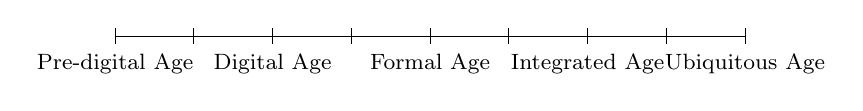
\begin{tikzpicture}
    \draw (0,0) -- (8,0);
    \foreach \x in {0,1,...,8} {
      \draw (\x,-0.1) -- (\x,0.1);
    }
    \foreach \x/\y in {0/Pre-digital Age, 2/Digital Age, 4/Formal Age, 6/Integrated Age, 8/Ubiquitous Age} {
      \node[anchor=north] at (\x,-0.1) {\footnotesize\y};
    }
  \end{tikzpicture}
  \caption{
    Timeline of the ages of data collection.
  }
  \label{fig:collection-history}
\end{figure}

\Cref{fig:collection-history} illutrates the timeline.

\subsubsection{Pre-digital age}

We can consider the earliest records of data collection to be the notches on sticks and
bones to keep tracking of passing of time.  The Lebombo bone, a baboon fibula with
notches, is probably the earliest known mathematical object.  It was found in the Lebombo
Mountains located between South Africa and Eswatini.
They estimate it is more
than 40,000 years old. It is conjectured to be a tally stick, but its exact purpose is
unknown. Its 29 notches suggests that may have been used as a lunar phase counter.
However, since it is broken at one end, the 29 notches may or may not be the total
number\footcite{Beaumont2013}.

Since the early forms of writing, humanity abilities to record events and information
increased significantly.  The first known written records date back to 3,500 BC, the
Sumerian archaic (pre-cuneiform) writing.  This writing system was used to represent
commodities using clay tokens and to record transactions\footcite{Ifrah1998}.

Another important milestone in the history of data collection is the record of
demographic data.  One of first known census was conducted in 3,800 BC in the Babylonian
Empire.  It was ordered to assess the population and resources of
his empire\footcite{Grajalez2013}.

Moving forward many years, I consider a major influential figure in the history of data
collection to be Florence Nightingale (1820 -- 1910).  She was a passionate statistician
and probably the first person to use statistics to influence public and official
opinion.  The meticulous records she kept during the Crimean War
(1853 -- 1856) were the evidence that saved lives.  She was also the first to use
statistical graphics to present data in a way that was easy to understand.  She is
credited with developing a form of the pie chart now known as the polar area
diagram.  She also reformed healthcare in the United Kingdom and
is considered the founder of modern nursing\footcite{Grajalez2013}.

\begin{mainbox}{Florence Nightingale}
  \begin{itemize}
    \item Passionate statistician.
    \item First person to use statistics to influence public and official opinion.
    \item Organized data from garden fruits and vegetables into numerical tables at the age of 9.
    \item At 20 she was receiving two-hour lessons from a Cambridge-trained mathematician.
    \item She found the sight of a long column of figures “perfectly reviving”.
    \item She went out to the Crimean War, to Scutari in Turkey, in 1854.
    \item She found that not even the numbers of soldiers entering the hospitals, or leaving them – alive or dead – was known.
    \item From the first she kept meticulous records.
    \item The data she collected was the evidence that saved lives.
    \item She was the first to use statistical graphics to present data in a way that was easy to understand.
    \item She is credited with developing a form of the pie chart now known as the polar area diagram.
    \item She reformed healthcare in the United Kingdom and is considered the founder of modern nursing.
  \end{itemize}
\end{mainbox}

\subsection{Timeline of data analysis}

\begin{itemize}
  \item Summary statistics
  \item Probability Advent 17, 18th
  \item Statistical learning 19th
    \begin{itemize}
      \item Bayes rule
      \item Gauss’ method of least squares
      \item Playfair data visualization
    \end{itemize}
  \item 20th inference
    \begin{itemize}
      \item Pearson hypothesis testing
      \item Fisher multivariate analysis, maximum likelihood estimate
    \end{itemize}
  \item Computer: McCulloch Pitts, Shannon information theory, Fix and Hodged discriminatory analysis, knn
  \item Machine learning: 1965 Nils Nilsson neural network, 1966 Hunt inducing trees, Kmeans, Vapnik 71
  \item Today: Ensembles, Deep learning: vision and language, KDD
\end{itemize}

% slides/fundamental.tex - Chapter 2: Fundamental Concepts

% slides/preamble.tex - Shared preamble for all slide decks
% Metropolis theme with grayscale style matching the book

\documentclass[aspectratio=169]{beamer}

\usetheme{metropolis}

% ---------- Colors (grayscale) ----------
\definecolor{bookdark}{gray}{0.2}
\definecolor{bookgray}{gray}{0.5}
\definecolor{booklight}{gray}{0.92}

\setbeamercolor{normal text}{fg=bookdark, bg=white}
\setbeamercolor{alerted text}{fg=bookdark}
\setbeamercolor{frametitle}{fg=white, bg=bookdark}
\setbeamercolor{title separator}{fg=bookgray}
\setbeamercolor{progress bar}{fg=bookgray, bg=booklight}
\setbeamercolor{block title}{fg=white, bg=bookgray}
\setbeamercolor{block body}{fg=bookdark, bg=booklight}
\setbeamercolor{block title alerted}{fg=white, bg=bookdark}
\setbeamercolor{block body alerted}{fg=bookdark, bg=booklight}
\setbeamercolor{block title example}{fg=white, bg=bookgray}
\setbeamercolor{block body example}{fg=bookdark, bg=booklight}

\setbeamertemplate{frame numbering}[fraction]

% ---------- Fonts (matching the book) ----------
\usepackage[T1]{fontenc}
\usepackage{fontspec}
\usepackage[warnings-off={mathtools-colon,mathtools-overbracket}]{unicode-math}

\setmathfont{STIXTwoMath}[
  Extension={.otf},
  Path={./fonts/},
  Scale=1]

\setsansfont{STIXTwoText}[
  Extension={.otf},
  Path={./fonts/},
  UprightFont={*-Regular},
  BoldFont={*-Bold},
  ItalicFont={*-Italic},
  BoldItalicFont={*-BoldItalic}]

\setmainfont{STIXTwoText}[
  Extension={.otf},
  Path={./fonts/},
  UprightFont={*-Regular},
  BoldFont={*-Bold},
  ItalicFont={*-Italic},
  BoldItalicFont={*-BoldItalic}]

\setmonofont{CourierPrime}[
  Extension={.ttf},
  Path={./fonts/},
  UprightFont={*-Regular},
  BoldFont={*-Bold},
  ItalicFont={*-Italic},
  BoldItalicFont={*-BoldItalic},
  Scale=0.9]

% ---------- Packages ----------
\usepackage{amsmath}
\usepackage{mathtools}
\usepackage{graphicx}
\usepackage{booktabs}

% ---------- TikZ ----------
\usepackage{tikz}
\usetikzlibrary{shapes, arrows.meta, positioning, shapes.geometric, fit}

\tikzset{%
  decision/.style={draw, diamond, text centered, minimum height=0.5cm, minimum width=1cm},
  block/.style={rectangle, draw, text width=6em, text centered, rounded corners, minimum height=3em},
  mediumblock/.style={rectangle, draw, text width=3em, text centered, rounded corners, minimum height=2em},
  darkblock/.style={block, fill=gray, text=white},
  smallblock/.style={rectangle, rounded corners, draw, font=\tiny, minimum height=1em, inner sep=2pt},
  smalldarkblock/.style={smallblock, fill=gray, text=white},
  darkcircle/.style={draw, circle, fill=gray, text centered, text=white},
  smallcircle/.style={draw, circle, text centered, font=\tiny},
  smalldarkcircle/.style={smallcircle, fill=gray, text=white},
  line/.style={draw, -latex},
  dline/.style={draw, latex-latex},
  bigarrow/.style={draw, -latex, line width=3pt, gray},
}

% ---------- Math operators ----------
\DeclareMathOperator*{\argmax}{arg\,max}
\DeclareMathOperator*{\argmin}{arg\,min}
\DeclareMathOperator{\Prob}{P}
\DeclareMathOperator{\E}{E}
\DeclareMathOperator{\Var}{Var}
\DeclareMathOperator{\sign}{sign}
\DeclareMathOperator{\clamp}{clamp}

% ---------- Hyperref ----------
\usepackage{hyperref}
\hypersetup{colorlinks, urlcolor=bookgray, linkcolor=bookdark}

% ---------- Commands ----------
\renewcommand{\vec}[1]{\mathbf{#1}}
\newcommand{\code}[1]{\colorbox{black!10!white}{\texttt{#1}}}

% ---------- Book info, license, and disclaimer ----------
\newcommand{\bookframe}{%
  \begin{frame}{About these slides}
    These slides are companion material for the book

    \vspace{0.3cm}
    \begin{center}
      \textbf{Data Science Project: An Inductive Learning Approach}\\[2pt]
      Prof.~Dr.~Filipe A. N. Verri\\[4pt]
      \url{https://leanpub.com/dsp}
    \end{center}

    \vspace{0.3cm}
    All intellectual content comes from the book and is not AI-generated.
    Slides were produced with the assistance of
    \href{https://claude.ai/code}{Claude Code}.

    \vspace{0.3cm}
    {\small
    Licensed under
    \href{https://creativecommons.org/licenses/by-nc/4.0/}{CC BY-NC 4.0}.
    You are free to modify and redistribute this work as long as you give
    proper credit and do not use it for commercial purposes.}
  \end{frame}%
}

% ---------- TikZ color presets (used by book figures) ----------
\colorlet{circle edge}{black!50}
\colorlet{circle area}{black!20}
\tikzset{
  filled/.style={fill=circle area, draw=circle edge, thick},
  outline/.style={draw=circle edge, thick},
}


\title{Fundamental Concepts}
\subtitle{Data Science Project: An Inductive Learning Approach}
\author{Prof.~Dr.~Filipe A. N. Verri}
\date{}

\begin{document}

\maketitle
\bookframe

% ---- Epigraph ----

\begin{frame}{}
  \vfill
  \begin{quote}
    The simple believes everything,\\
    but the prudent gives thought to his steps.
    \begin{flushright}
      --- Proverbs 14:15 (ESV)
    \end{flushright}
  \end{quote}
  \vfill
\end{frame}

% ---- Overview ----

\begin{frame}{Overview}
  \begin{columns}[T]
    \begin{column}{0.48\textwidth}
      \textbf{Contents}
      \begin{itemize}
        \item Data science definition
        \item The data science continuum
        \item Fundamental data theory
      \end{itemize}
    \end{column}
    \begin{column}{0.48\textwidth}
      \textbf{Objectives}
      \begin{itemize}
        \item Define data science
        \item Present the main concepts about data theory
      \end{itemize}
    \end{column}
  \end{columns}
\end{frame}

% ===========================================================================
\section{Data science definition}
% ===========================================================================

\begin{frame}{Definitions in the literature}
  \begin{itemize}
    \item \textbf{Zumel \& Mount:} cross-disciplinary practice drawing on data
      engineering, statistics, data mining, ML, and predictive analytics
    \item \textbf{Wickham \& Grolemund:} discipline that transforms raw data into
      understanding, insight, and knowledge
    \item \textbf{Hayashi:} not only unifies statistics and data analysis, but
      intends to analyze and understand actual phenomena with data
  \end{itemize}
\end{frame}

\begin{frame}{Our definition}
  \begin{block}{Definition: Data science}
    Data science is the study of knowledge extraction from measurable phenomena
    using computational methods.
  \end{block}

  \vspace{0.5cm}
  Key terms:
  \begin{itemize}
    \item \textbf{Computational methods} --- use computers to handle data
    \item \textbf{Knowledge} --- information humans can understand and apply
    \item \textbf{Measurable phenomena} --- events we can quantify
    \item \textbf{Raw data} --- collected directly, not yet transformed
  \end{itemize}
\end{frame}

\begin{frame}{Data science vs conventional sciences}
  \begin{itemize}
    \item Conventional: named after object of study (biology $\to$ life)
    \item Data science: studies \textit{how} to extract knowledge from data
    \item Similar to ``computer science'' --- not the study of computers
    \item Conventional paradigm: model-driven (observe, hypothesize, validate)
    \item Data science paradigm: data-driven (extract knowledge from data)
    \item We give data the opportunity to \textbf{surprise us}
  \end{itemize}
\end{frame}

% ---- Figure: My view of data science ----

\def\verrids{(0,0) circle (20mm)}
\def\verrist{(-2.5,0) circle (15mm)}
\def\verride{(2.5,0) circle (15mm)}
\def\verrics{(0,-2.5) circle (15mm)}

\begin{frame}{My view of data science}
  \centering
  \begin{tikzpicture}
    \begin{scope}
      \clip \verrids;
      \fill[filled] \verrist;
      \fill[filled] \verride;
      \fill[filled] \verrics;
    \end{scope}
    \draw[outline] \verrids node(ds) {};
    \draw[outline] \verrist node {Statistics};
    \draw[outline, text width=27mm, text centered] \verride node {Philosophy / domain expertise};
    \draw[outline] \verrics node {Computer science};
    \node[anchor=north,above] at (0, 1) {Data science};
  \end{tikzpicture}

  \vspace{0.3cm}
  \small An entirely new science --- its basis comes from other sciences,\\
  but its object of study is particular enough to raise new questions.
\end{frame}

% ===========================================================================
\section{The data science continuum}
% ===========================================================================

\begin{frame}{From borrowed methods to a new science}
  \begin{itemize}
    \item Object of study in data science is not new
    \item Key factor: social demand and importance of data
    \item ``Data is the new oil''
    \item Methods develop $\to$ experiments validate $\to$ credibility grows
    \item Academic recognition: new courses and programs
    \item Unique questions emerge, distinct from parent disciplines
  \end{itemize}
\end{frame}

% ---- Figure: The data science continuum ----

\begin{frame}{The data science continuum}
  \centering
  \begin{tikzpicture}[node distance=4mm and 5mm, scale=0.88, transform shape]
    % Left: Established Sciences
    \node (stats) [mediumblock, text width=1.8cm] {Statistics};
    \node (cs) [mediumblock, text width=1.8cm, below=of stats] {Computer science};
    \node (ds) [mediumblock, text width=1.8cm, below=of cs] {Philosophy and others};
    \node (basebox) [draw, dashed, inner sep=0.3cm, fit={(stats) (ds)},
      label=above:{\small Established sciences}] {};
    % Flow to the right
    \node (principles) [darkblock, right=of basebox, text width=2cm,
      minimum height=2em] {Emergence of principles};
    \node (methods) [block, right=of principles, text width=2cm,
      minimum height=2em] {Unique methods};
    \node (validation) [darkblock, right=of methods, text width=2cm,
      minimum height=2em] {Validation and new challenges};
    \node (science) [block, right=of validation, text width=2cm,
      minimum height=2em] {Data science};
    % Arrows
    \draw[-{Stealth}] (basebox) -- (principles);
    \draw[-{Stealth}] (principles) -- (methods);
    \draw[-{Stealth}] (methods) -- (validation);
    \draw[-{Stealth}] (validation) -- (science);
  \end{tikzpicture}
\end{frame}

\begin{frame}{New questions in data science}
  \begin{itemize}
    \item How can we guarantee that the data is reliable?
    \item How can we collect data without biasing conclusions?
    \item How can we guarantee that data usage is ethical?
    \item How can we present results to non-experts?
  \end{itemize}
\end{frame}

% ===========================================================================
\section{Fundamental data theory}
% ===========================================================================

% ---------------------------------------------------------------------------
\subsection{Phenomena}
% ---------------------------------------------------------------------------

\begin{frame}{Phenomena and philosophy}
  \begin{itemize}
    \item Phenomenon: any observable event or process
    \item \textbf{Ontology} --- study of being, existence, categories
    \item \textbf{Epistemology} --- study of knowledge and justification
    \item \textbf{Logic} --- study of reasoning and inference
  \end{itemize}

  \vspace{0.5cm}
  Understanding phenomena requires both general philosophical
  knowledge and domain expertise.
\end{frame}

\begin{frame}{Aristotle's categories}
  \begin{itemize}
    \item Aristotle (384--322 BC) --- first systematic classification
    \item Ten categories: substance, quantity, quality, relation, place, time, \ldots
    \item Practical view: focus on the world we can perceive
    \item Foundation of logical reasoning and scientific classification
    \item Still used in computer and data systems
  \end{itemize}
\end{frame}

\begin{frame}{Why ontology matters for data science}
  \begin{itemize}
    \item Describing = reducing complexity to simple pieces
    \item Phenomena $\approx$ substance; data $\approx$ properties, relations, states
    \item Identifying entities and their properties $\to$ better data collection
    \item Understanding logical limitations avoids errors
    \item Common mistake: assuming columns with the same name have the same meaning
  \end{itemize}
\end{frame}

% ---------------------------------------------------------------------------
\subsection{Measurements}
% ---------------------------------------------------------------------------

\begin{frame}{Measurements}
  \begin{itemize}
    \item Data science focuses on \textbf{measurable phenomena}
    \item Data collection: systematic gathering of data on a phenomenon
    \item Systematic $=$ planned, with understood consequences
    \item \textbf{Sampling bias} --- influence of the collection method on conclusions
    \item Data storage: digitally storing collected data
  \end{itemize}
\end{frame}

\begin{frame}{Data types}
  \begin{itemize}
    \item Data types must correctly reflect the source phenomenon
    \item Data types restrict the operations we can perform
    \item Foundations from computer science:
      \begin{itemize}
        \item Algorithms and data structures
        \item Databases
      \end{itemize}
    \item Concepts are independent of programming language or RDBMS
  \end{itemize}
\end{frame}

% ---------------------------------------------------------------------------
\subsection{Knowledge extraction}
% ---------------------------------------------------------------------------

\begin{frame}{Reasoning}
  \begin{itemize}
    \item \textbf{Deductive reasoning} --- from general rules to specific conclusions
    \item \textbf{Inductive reasoning} --- from specific observations to general rules
    \item Data science relies on \textbf{inductive reasoning}
    \item Descartes: algebra to mechanize reasoning
    \item Leibniz: universal algebraic language for logical methods
  \end{itemize}
\end{frame}

\begin{frame}{Knowledge extraction methods}
  \begin{itemize}
    \item \textbf{Statistics} --- collection, organization, analysis, interpretation
    \item \textbf{Machine learning} --- algorithms that learn from data automatically
    \item \textbf{Operations research} --- computational methods to optimize decisions
    \item Domain-specific methods: bioinformatics, geoinformatics, \ldots
    \item Each method has its own assumptions and limitations
  \end{itemize}
\end{frame}

\begin{frame}{Data preprocessing}
  \begin{itemize}
    \item When data do not match the method's requirements
    \item \textbf{Data cleaning} --- detecting and correcting corrupt data
    \item \textbf{Data transformation} --- converting formats or types
    \item \textbf{Data enhancement} --- integrating data from different sources
    \item Methods are usually robust to imperfections, but preprocessing helps
  \end{itemize}
\end{frame}

% ---- Takeaways ----

\begin{frame}{Takeaways}
  \begin{itemize}
    \item Data science is a new science that studies knowledge extraction
      from measurable phenomena using computational methods
    \item The data science continuum: from borrowed methods to a distinct discipline
    \item Understanding phenomena, measurements, and knowledge extraction
      is fundamental
  \end{itemize}
\end{frame}

% ---- End ----

\begin{frame}[standout]
  Questions?
\end{frame}

\end{document}

\chapter{Data science project}

\chapterprecishere{Figured I could throw myself a pity party or go back to school and
learn the computers. \par\raggedleft--- \textup{Don Carlton}, Monsters University (2013)}

First of all, a data science project is a software project.  The difference between a data
science software and a traditional software is that some components of the former is
constructed from data.  This means that part of the solution cannot be designed from the
knowledge of the domain expert, but must be learned from the data.  (Alternatively, the
cost of designing the solution is too high, and it is more efficient to learn it from the data.)

One good example of a data science project is a spam filter.  The spam filter is a software
that classifies emails into two categories: spam and non-spam.  The software is trained
using a set of emails that are already classified as spam or non-spam.  The software is
then used to classify new emails.  The software is a data science software because the
classification algorithm is learned from the data, i.e. the filters are not designed ``by
hand''.

% TODO:
% - the need of methodologies for data science projects
% - CRISP-DM
% - Nina's approach
% - Agile
% - Problems and advantages of SCRUM
% - Our approach

\section{CRISP-DM}

CRISP-DM\footnote{Official guide available at
\url{https://www.ibm.com/docs/it/SS3RA7_18.3.0/pdf/ModelerCRISPDM.pdf}.} is a methodology
for data mining projects.  It is an acronym for Cross Industry Standard Process for Data
Mining.  It is a methodology that was developed in the 1990s by IBM, and it is still
widely used today.

CRISP-DM is a cyclic process.  The process is composed of six phases:
\begin{enumerate}
  \item Business understanding: this is the phase where the project objectives are
    defined.  The objectives must be defined in a way that is measurable.  The phase also
    includes the definition of the project plan.
  \item Data understanding: this is the phase where the data is collected and explored.
    The data is collected from the data sources, and it is explored to understand its
    characteristics.  The phase also includes the definition of the data quality
    requirements.
  \item Data preparation: this is the phase where the data is prepared for the modeling
    phase.  The data is cleaned, transformed, and aggregated.  The phase also includes the
    definition of the modeling requirements.
  \item Modeling: this is the phase where the model is trained and validated.  The model is
    trained using the prepared data, and it is validated using the validation data.  The
    phase also includes the definition of the evaluation requirements.
  \item Evaluation: this is the phase where the model is evaluated.  The model is evaluated
    using the evaluation data.  The phase also includes the definition of the deployment
    requirements.
  \item Deployment: this is the phase where the model is deployed.  The model is deployed
    using the deployment requirements.  The phase also includes the definition of the
    monitoring requirements.
\end{enumerate}

\Cref{fig:cripdm} shows a diagram of the CRISP-DM process.  Note that the process is
cyclic and completly focused on the data.  The process do not address the software
development aspects of the project.

\begin{figurebox}[label=fig:cripdm]{Diagram of the CRISP-DM process.}
  \centering
  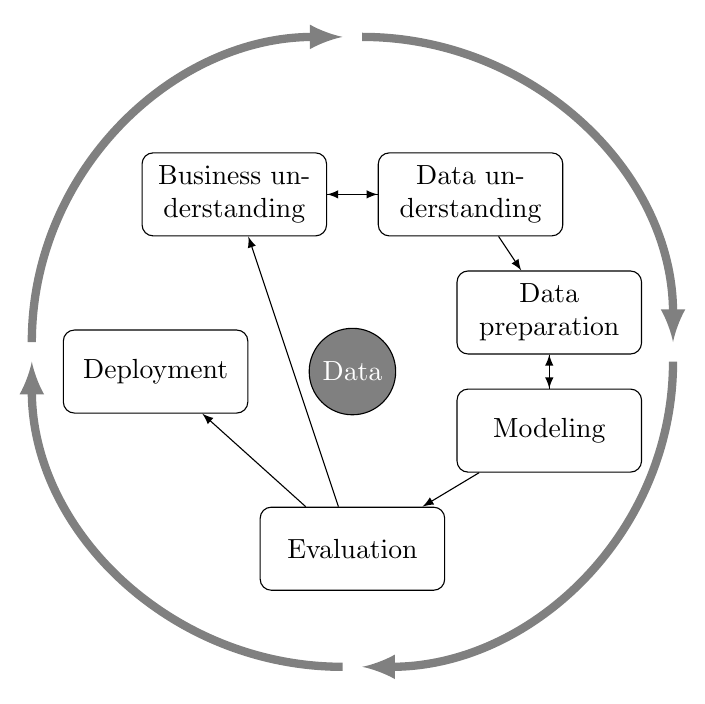
\begin{tikzpicture}[%
      block/.style={rectangle, draw, fill=white!20, text width=6em, text centered, rounded corners, minimum height=3em},
      line/.style={draw, -latex},
      bigarrow/.style={draw, -latex, line width=3pt, gray}
      ]
    \node (1) at (0, 0) {};
    \node (2) at (4, -4) {};
    \node (3) at (0, -8) {};
    \node (4) at (-4, -4) {};

    \node [block] (bu) at (-1.5, -2) {Business understanding};
    \node [block] (du) at (1.5, -2) {Data understanding};
    \path [line] (bu) -- (du);
    \path [line] (du) -- (bu);

    \node [block] (dp) at (2.5, -3.5) {Data preparation};
    \node [block] (m) at (2.5, -5) {Modeling};
    \path [line] (dp) -- (m);
    \path [line] (m) -- (dp);

    \path [line] (du) -- (dp);

    \node [block] (e) at (0, -6.5) {Evaluation};
    \node [block] (d) at (-2.5, -4.25) {Deployment};

    \path [line] (m) -- (e);
    \path [line] (e) -- (d);
    \path [line] (e) -- (bu);

    \node [draw, circle, fill=gray, text centered, text=white] at (0, -4.25) {Data};

    \path [bigarrow] (1.east) to[out=0, in=90] (2.60);
    \path [bigarrow] (2.-60) to[out=-90, in=0] (3.east);
    \path [bigarrow] (3.west) to[out=180, in=-90] (4.-120);
    \path [bigarrow] (4.120) to[out=90, in=180] (1.west);
  \end{tikzpicture}
  \tcblower
  Each block represents a phase of the CRISP-DM process.  Data is the central element of
  the process.  Arrows represent the transitions between the phases.
\end{figurebox}

The CRISP-DM methodology is a good starting point for data science projects.  However, it
does not mean that should be followed strictly.  The process is cyclic and flexible, and
adaptations are possible at any stage of the process.

\section{Nina and Zumel's approach}

\textcite{Zumel2019} propose a methodology for data science projects.

They define five roles:
\begin{itemize}
  \item Project sponsor: represents the business interests and champions the project;
  \item Client: represents the end users’ interests and is the domain expert;
  \item Data scientist: sets and executes the analytic strategy and communicates with the
    sponsor and the client;
  \item Data architect: manages data and data storage and sometimes manages data
    collection;
  \item Operations: manages infrastructure and deploys final project results.
\end{itemize}

\citeauthor{Zumel2019}'s model is similar to CRISP-DM, but emphasizes that back-and-forth
is possible at any stage of the process.

\section{Agile}

Agile is a methodology for software development.  It is an alternative to the waterfall
methodology.  The waterfall methodology is a sequential design where each phase
must be completed before the next phase can begin.

The four values of agile manifesto are:
\begin{itemize}
  \item Individuals and interactions over processes and tools;
  \item Working software over comprehensive documentation;
  \item Customer collaboration over contract negotiation;
  \item Responding to change over following a plan.
\end{itemize}

\section{SCRUM}

SCRUM is an agile framework for software development.  It is a process framework for
managing complex projects.  It is a lightweight process framework, which means that it
provides just enough guidance to be effective.

Many consider that SCRUM is not adequate for data science projects.  The main reason is
that SCRUM is designed for projects where the requirements are known in advance.  Also,
that data science projects have exploratory phases, which are not well supported by SCRUM.

I argue that this view is wrong.  SCRUM is a framework, and it is designed to be adapted to
the needs of the project.  SCRUM is not a rigid process.  In the following, I propose an
extension to SCRUM that makes it suitable for data science projects.

(In real-world, most developers do not have hacking-level skills.  They are not autonomous
enough to work without a plan.  This is especially true for ``data scientists'', who are
often not even developers.  SCRUM is a good compromise between the need for autonomy and
the need for a detailed plan.  Project methodology is needed to ensure that the project is
completed in time and within budget.)

\section{Our approach}

We propose an extension to SCRUM that makes it suitable for data science projects.  The
extension is based on the following observations:
\begin{itemize}
  \item Data science projects have exploratory phases;
  \item \dots
\end{itemize}

Two other values must be added to the agile manifesto:
\begin{itemize}
  \item Model confidence/understanding over model performance;
  \item Beware of interactive environments.
\end{itemize}

\subsection{The roles}

Combine SCRUM roles with the roles defined by \textcite{Zumel2019}.

\subsection{The principles of our approach}

\begin{enumerate}
  \item Modularize the solution. Usually, in four main modules: frontend, backend,
    dataset, and model search.  The frontend is the user interface.  The backend is the
    server-side code.  The dataset is the data that is used to train the model.  The model
    search is the code that searches for the best model.
  \item Version control everything.  This includes the code, the data, and the
    documentation. The most used tool for code version control is Git.  For datasets,
    extensions to Git exist, such as DVC\footnote{\url{https://dvc.org/}}.  One important aspect
    is to version control the model search code.  Interactive environments such as Jupyter
    notebooks are not suitable for this purpose.  They can be used to draft the code, but
    the final version must be version controlled.
  \item Continuous integration and continuous deployment.  This means that the code is
    automatically (or at least semi-automatically) tested and deployed.  The backend and
    frontend code is tested using unit tests.  The model search code is tested using
    validation methods such as cross-validation and Bayesian analysis on the discovered
    models.  Usually the model search code is very computationally intensive, and it is
    not feasible to run it on every commit.  Instead, it is run periodically, for example
    once a day.  If the clould infrastructure required to run the model search code is not
    available to automate validation and deploymen, at least make sure that the code is
    easily runnable.  This means that the code must be well documented, and that the
    required infrastructure must be well documented.  Also aggregate commands using a
    Makefile or a similar tool.  Pay attention on the dependences between dataset and the
    model training.  If the dataset changes significantly, not only the deployed model
    must be retrained, but the model search algorithm may need to be rethought.
  \item Reports as deliverables.  During sprints, the deliverables of data exploration are
    reports.
  \item Setup quantitative goals.  Do not fall on the trap of forever improving the model.
    Instead, setup quantitative goals for the model performance.  For example, the model
    must have a precision of at least 90\%.  Once you reach the goal, prioritize other
    tasks.
  \item Measure \emph{exactly} what you want.  During model validation, use your own
    metrics based on the project goals.  Usually, more than one metric is needed, and they
    might be conflicting.  Use strategies to balance the metrics, such as Pareto
    optimization.  Beware of the metrics that are most used in the literature.  They might not
    be suitable for your project.  Notice that during model training, some methods are
    limited to the loss functions that they can optimize.  If possible, choose a method
    that can optimize the loss function that you want.  Even if you are not explicitly
    optimizing the wanted metric, you might find a model that performs well on that metric.
    That is a reason validation is important.
  \item Report model stability and performance variance.  Understanding the limitations
    and characteristics of the model is more important than the model performance.  For
    example, if the model performance is high, but the model is unstable, it is not
    suitable for production.  Also, in some scenarios, interpretability is more important than
    performance.
  \item In user interface, mask data-science-specific terminology.  Usually, data science
    software gives the user the option to choose the model.  In order to avoid confusion,
    the user interface must mask the data-science-specific terminology.  This helps non
    experts to use the software consciously.
  \item Monitor model performance in production.  If possible setup feedback from the user
    interface.  Avoid automation of model releases because concept drift usually requires
    exploratory analysis.
  \item Use the appropriate backend.  REST API vs websocket.
\end{enumerate}

% slides/structured-data.tex - Chapter 4: Structured Data

% slides/preamble.tex - Shared preamble for all slide decks
% Metropolis theme with grayscale style matching the book

\documentclass[aspectratio=169]{beamer}

\usetheme{metropolis}

% ---------- Colors (grayscale) ----------
\definecolor{bookdark}{gray}{0.2}
\definecolor{bookgray}{gray}{0.5}
\definecolor{booklight}{gray}{0.92}

\setbeamercolor{normal text}{fg=bookdark, bg=white}
\setbeamercolor{alerted text}{fg=bookdark}
\setbeamercolor{frametitle}{fg=white, bg=bookdark}
\setbeamercolor{title separator}{fg=bookgray}
\setbeamercolor{progress bar}{fg=bookgray, bg=booklight}
\setbeamercolor{block title}{fg=white, bg=bookgray}
\setbeamercolor{block body}{fg=bookdark, bg=booklight}
\setbeamercolor{block title alerted}{fg=white, bg=bookdark}
\setbeamercolor{block body alerted}{fg=bookdark, bg=booklight}
\setbeamercolor{block title example}{fg=white, bg=bookgray}
\setbeamercolor{block body example}{fg=bookdark, bg=booklight}

\setbeamertemplate{frame numbering}[fraction]

% ---------- Fonts (matching the book) ----------
\usepackage[T1]{fontenc}
\usepackage{fontspec}
\usepackage[warnings-off={mathtools-colon,mathtools-overbracket}]{unicode-math}

\setmathfont{STIXTwoMath}[
  Extension={.otf},
  Path={./fonts/},
  Scale=1]

\setsansfont{STIXTwoText}[
  Extension={.otf},
  Path={./fonts/},
  UprightFont={*-Regular},
  BoldFont={*-Bold},
  ItalicFont={*-Italic},
  BoldItalicFont={*-BoldItalic}]

\setmainfont{STIXTwoText}[
  Extension={.otf},
  Path={./fonts/},
  UprightFont={*-Regular},
  BoldFont={*-Bold},
  ItalicFont={*-Italic},
  BoldItalicFont={*-BoldItalic}]

\setmonofont{CourierPrime}[
  Extension={.ttf},
  Path={./fonts/},
  UprightFont={*-Regular},
  BoldFont={*-Bold},
  ItalicFont={*-Italic},
  BoldItalicFont={*-BoldItalic},
  Scale=0.9]

% ---------- Packages ----------
\usepackage{amsmath}
\usepackage{mathtools}
\usepackage{graphicx}
\usepackage{booktabs}

% ---------- TikZ ----------
\usepackage{tikz}
\usetikzlibrary{shapes, arrows.meta, positioning, shapes.geometric, fit}

\tikzset{%
  decision/.style={draw, diamond, text centered, minimum height=0.5cm, minimum width=1cm},
  block/.style={rectangle, draw, text width=6em, text centered, rounded corners, minimum height=3em},
  mediumblock/.style={rectangle, draw, text width=3em, text centered, rounded corners, minimum height=2em},
  darkblock/.style={block, fill=gray, text=white},
  smallblock/.style={rectangle, rounded corners, draw, font=\tiny, minimum height=1em, inner sep=2pt},
  smalldarkblock/.style={smallblock, fill=gray, text=white},
  darkcircle/.style={draw, circle, fill=gray, text centered, text=white},
  smallcircle/.style={draw, circle, text centered, font=\tiny},
  smalldarkcircle/.style={smallcircle, fill=gray, text=white},
  line/.style={draw, -latex},
  dline/.style={draw, latex-latex},
  bigarrow/.style={draw, -latex, line width=3pt, gray},
}

% ---------- Math operators ----------
\DeclareMathOperator*{\argmax}{arg\,max}
\DeclareMathOperator*{\argmin}{arg\,min}
\DeclareMathOperator{\Prob}{P}
\DeclareMathOperator{\E}{E}
\DeclareMathOperator{\Var}{Var}
\DeclareMathOperator{\sign}{sign}
\DeclareMathOperator{\clamp}{clamp}

% ---------- Hyperref ----------
\usepackage{hyperref}
\hypersetup{colorlinks, urlcolor=bookgray, linkcolor=bookdark}

% ---------- Commands ----------
\renewcommand{\vec}[1]{\mathbf{#1}}
\newcommand{\code}[1]{\colorbox{black!10!white}{\texttt{#1}}}

% ---------- Book info, license, and disclaimer ----------
\newcommand{\bookframe}{%
  \begin{frame}{About these slides}
    These slides are companion material for the book

    \vspace{0.3cm}
    \begin{center}
      \textbf{Data Science Project: An Inductive Learning Approach}\\[2pt]
      Prof.~Dr.~Filipe A. N. Verri\\[4pt]
      \url{https://leanpub.com/dsp}
    \end{center}

    \vspace{0.3cm}
    All intellectual content comes from the book and is not AI-generated.
    Slides were produced with the assistance of
    \href{https://claude.ai/code}{Claude Code}.

    \vspace{0.3cm}
    {\small
    Licensed under
    \href{https://creativecommons.org/licenses/by-nc/4.0/}{CC BY-NC 4.0}.
    You are free to modify and redistribute this work as long as you give
    proper credit and do not use it for commercial purposes.}
  \end{frame}%
}

% ---------- TikZ color presets (used by book figures) ----------
\colorlet{circle edge}{black!50}
\colorlet{circle area}{black!20}
\tikzset{
  filled/.style={fill=circle area, draw=circle edge, thick},
  outline/.style={draw=circle edge, thick},
}


\title{Structured Data}
\subtitle{Data Science Project: An Inductive Learning Approach}
\author{Prof.~Dr.~Filipe A. N. Verri}
\date{}

\begin{document}

\maketitle
\bookframe

% ---- Epigraph ----

\begin{frame}{}
  \vfill
  \begin{quote}
    Like families, tidy datasets are all alike, but every messy dataset is
    messy in its own way.
    \begin{flushright}
      --- Hadley Wickham, \textit{Tidy Data}
    \end{flushright}
  \end{quote}
  \vfill
\end{frame}

% ---- Overview ----

\begin{frame}{Overview}
  \begin{columns}[T]
    \begin{column}{0.48\textwidth}
      \textbf{Contents}
      \begin{itemize}
        \item Data types
        \item Database normalization
        \item Tidy data
        \item Bridging normalization and tidiness
        \item Data semantics and interpretation
      \end{itemize}
    \end{column}
    \begin{column}{0.48\textwidth}
      \textbf{Objectives}
      \begin{itemize}
        \item Understand common data types and formats
        \item Associate data format and semantics
        \item Enable the reader to perform data tasks well
      \end{itemize}
    \end{column}
  \end{columns}
\end{frame}

% ===========================================================================
\section{Data types}
% ===========================================================================

\begin{frame}{Stevens' types}
  \centering
  \rowcolors{2}{black!10!white}{}
  \begin{tabular}{ll}
    \toprule
    \textbf{Data type} & \textbf{Allowed operations} \\
    \midrule
    Nominal  & $=$ \\
    Ordinal  & $=, <$ \\
    Interval & $=, <, +, -$ \\
    Ratio    & $=, <, +, -, \times, \div$ \\
    \bottomrule
  \end{tabular}

  \vspace{0.5cm}
  \small
  \begin{tabular}{ll}
    Nominal:  & colors \\
    Ordinal:  & small $<$ medium $<$ large \\
    Interval: & temperature in Celsius \\
    Ratio:    & weight in kilograms \\
  \end{tabular}
\end{frame}

\begin{frame}{Limitations of Stevens' types}
  \begin{itemize}
    \item Do not exhaust all possibilities (e.g., probabilities)
    \item Data types are not always evident from the data alone
    \item Same data can be interpreted differently depending on context
    \item Data scientists must be aware of types and their consequences
    \item Good assumptions and hypotheses are a key part of the methodology
  \end{itemize}
\end{frame}

% ===========================================================================
\section{Database normalization}
% ===========================================================================

% ---------------------------------------------------------------------------
\subsection{Relational algebra}
% ---------------------------------------------------------------------------

\begin{frame}{Relational algebra --- Concepts}
  \begin{itemize}
    \item \textbf{Relation} --- table with rows (tuples) and columns (attributes)
    \item \textbf{Projection} $\pi_{A,C}(X)$ --- select only specified columns
    \item \textbf{Join} $S \bowtie T$ --- combine relations on common attributes
    \item \textbf{Functional dependency} $U \to V$ --- if tuples agree on $U$,
      they agree on $V$
    \item \textbf{Multi-valued dependency} $U \twoheadrightarrow V$ ---
      $R = R[UV] \bowtie R[UW]$
    \item \textbf{Join dependency} $*\{X_1, \ldots, X_n\}$ ---
      $R = \bowtie\{R[X_1], \ldots, R[X_n]\}$
  \end{itemize}
\end{frame}

% ---------------------------------------------------------------------------
\subsection{Normal forms}
% ---------------------------------------------------------------------------

\begin{frame}{Normal forms}
  Progressive conditions to reduce redundancy:
  \begin{itemize}
    \item \textbf{1NF} --- all attributes are atomic
    \item \textbf{2NF} --- 1NF + non-prime attributes fully depend on primary key
    \item \textbf{3NF} --- 2NF + no transitive dependencies
    \item \textbf{BCNF} --- every functional dependency is a result of keys
    \item \textbf{4NF} --- every multi-valued dependency is a result of keys
    \item \textbf{PJNF} --- key dependencies imply all join dependencies
  \end{itemize}
\end{frame}

\begin{frame}{Example: 2NF vs 3NF}
  2NF (redundant ``course credits''):

  \centering
  \small
  \rowcolors{2}{black!10!white}{}
  \begin{tabular}{cccc}
    \toprule
    \textbf{Student} & \textbf{Course} & \textbf{Credits} & \textbf{Grade} \\
    \midrule
    Alice & Math & 4 & A \\
    Alice & Physics & 3 & B \\
    Bob & Math & 4 & B \\
    Bob & Physics & 3 & A \\
    \bottomrule
  \end{tabular}

  \vspace{0.4cm}
  \raggedright
  3NF (separate tables):

  \centering
  \rowcolors{2}{black!10!white}{}
  \begin{tabular}{cc}
    \toprule
    \textbf{Course} & \textbf{Credits} \\
    \midrule
    Math & 4 \\
    Physics & 3 \\
    \bottomrule
  \end{tabular}
  \quad
  \rowcolors{2}{black!10!white}{}
  \begin{tabular}{ccc}
    \toprule
    \textbf{Student} & \textbf{Course} & \textbf{Grade} \\
    \midrule
    Alice & Math & A \\
    Alice & Physics & B \\
    Bob & Math & B \\
    Bob & Physics & A \\
    \bottomrule
  \end{tabular}
\end{frame}

\begin{frame}{PJNF and invalid joins}
  \begin{itemize}
    \item Relation $R[ABC]$ with primary key $ABC$ (no non-trivial FDs)
    \item Constraint: if $(a,b,c')$, $(a,b',c)$, $(a',b,c) \in R$
      then $(a,b,c) \in R$
    \item Join dependency $*\{AB, AC, BC\}$ not implied by key
    \item Must split into $R_1[AB]$, $R_2[AC]$, $R_3[BC]$
    \item Careless joins may produce invalid tuples
  \end{itemize}
\end{frame}

% ===========================================================================
\section{Tidy data}
% ===========================================================================

\begin{frame}{Tidy data}
  A standardized way to organize data values (Wickham, 2014):
  \begin{itemize}
    \item Each \textbf{value} belongs to a variable and an observation
    \item Each \textbf{variable} (column) = same attribute across units
    \item Each \textbf{observation} (row) = same unit across attributes
    \item \textbf{Observational unit} = individual entity being measured
  \end{itemize}

  \vspace{0.3cm}
  \centering
  \small
  \rowcolors{2}{black!10!white}{}
  \begin{tabular}{cccc}
    \toprule
    \textbf{Concept} & \textbf{Structure} & \textbf{Contains} & \textbf{Across} \\
    \midrule
    Variable & Column & Same attribute & Units \\
    Observation & Row & Same unit & Attributes \\
    \bottomrule
  \end{tabular}
\end{frame}

\begin{frame}{Messy vs tidy}
  \begin{columns}[T]
    \begin{column}{0.48\textwidth}
      \textbf{Messy}\\[0.2cm]
      \centering\small
      \rowcolors{2}{black!10!white}{}
      \begin{tabular}{lcc}
        \toprule
         & \textbf{2019} & \textbf{2020} \\
        \midrule
        Brazil & 100 & 200 \\
        USA &  & 400 \\
        \bottomrule
      \end{tabular}
    \end{column}
    \begin{column}{0.48\textwidth}
      \textbf{Tidy}\\[0.2cm]
      \centering\small
      \rowcolors{2}{black!10!white}{}
      \begin{tabular}{lcc}
        \toprule
        \textbf{Country} & \textbf{Year} & \textbf{Cases} \\
        \midrule
        Brazil & 2019 & 100 \\
        Brazil & 2020 & 200 \\
        USA & 2019 & \\
        USA & 2020 & 400 \\
        \bottomrule
      \end{tabular}
    \end{column}
  \end{columns}

  \vspace{0.5cm}
  Tidy data: variables and observations are clear from the table itself.
\end{frame}

% ---------------------------------------------------------------------------
\subsection{Common messy datasets}
% ---------------------------------------------------------------------------

\begin{frame}{Problem: headers are values}
  \begin{columns}[T]
    \begin{column}{0.48\textwidth}
      \textbf{Messy} (Pew Forum)\\[0.2cm]
      \centering\scriptsize
      \rowcolors{2}{black!10!white}{}
      \begin{tabular}{lrrr}
        \toprule
        \textbf{Religion} & \textbf{<\$10k} & \textbf{\$10-20k} & \textbf{\dots} \\
        \midrule
        Agnostic & 27 & 34 & \dots \\
        Atheist & 12 & 27 & \dots \\
        Buddhist & 27 & 21 & \dots \\
        \bottomrule
      \end{tabular}
    \end{column}
    \begin{column}{0.48\textwidth}
      \textbf{Tidy}\\[0.2cm]
      \centering\scriptsize
      \rowcolors{2}{black!10!white}{}
      \begin{tabular}{llr}
        \toprule
        \textbf{Religion} & \textbf{Income} & \textbf{Freq.} \\
        \midrule
        Agnostic & <\$10k & 27 \\
        Agnostic & \$10-20k & 34 \\
        \dots & \dots & \dots \\
        Atheist & <\$10k & 12 \\
        Atheist & \$10-20k & 27 \\
        \dots & \dots & \dots \\
        \bottomrule
      \end{tabular}
    \end{column}
  \end{columns}

  \vspace{0.3cm}
  Table becomes longer but narrower.
\end{frame}

\begin{frame}{Problem: multiple variables in one column}
  \begin{columns}[T]
    \begin{column}{0.48\textwidth}
      \textbf{Messy} (TB dataset)\\[0.2cm]
      \centering\scriptsize
      \rowcolors{2}{black!10!white}{}
      \begin{tabular}{lllr}
        \toprule
        \textbf{country} & \textbf{year} & \textbf{column} & \textbf{cases} \\
        \midrule
        AD & 2000 & m014 & 0 \\
        AD & 2000 & m1524 & 0 \\
        AD & 2000 & m2534 & 1 \\
        \dots & \dots & \dots & \dots \\
        \bottomrule
      \end{tabular}
    \end{column}
    \begin{column}{0.48\textwidth}
      \textbf{Tidy}\\[0.2cm]
      \centering\scriptsize
      \rowcolors{2}{black!10!white}{}
      \begin{tabular}{lllllr}
        \toprule
        \textbf{country} & \textbf{year} & \textbf{sex} & \textbf{age} & \textbf{cases} \\
        \midrule
        AD & 2000 & m & 0--14 & 0 \\
        AD & 2000 & m & 15--24 & 0 \\
        AD & 2000 & m & 25--34 & 1 \\
        \dots & \dots & \dots & \dots & \dots \\
        \bottomrule
      \end{tabular}
    \end{column}
  \end{columns}

  \vspace{0.3cm}
  Same number of rows, but wider.
\end{frame}

\begin{frame}{Problem: variables in both rows and columns}
  \begin{itemize}
    \item Most complicated case of messy data
    \item One column contains variable names (e.g., ``element'' = tmax/tmin)
    \item Day columns (d1, d2, \ldots) are values, not variable names
    \item Fix: lengthen first, then widen by variable names
  \end{itemize}
\end{frame}

\begin{frame}{Problem: multiple observational units in one table}
  \begin{itemize}
    \item Common during data collection
    \item Example: billboard data with track info repeated for each week
    \item Fix: separate into one table per observational unit
    \item Create unique identifiers to link the tables
  \end{itemize}
\end{frame}

\begin{frame}{Problem: single unit in multiple tables}
  \begin{itemize}
    \item Data split across files (e.g., one file per year)
    \item Table/file itself represents a variable value
    \item Fix: make columns compatible, combine, add origin column
  \end{itemize}
\end{frame}

% ===========================================================================
\section{Bridging normalization, tidiness, and data theory}
% ===========================================================================

\begin{frame}{Bridge between concepts}
  \centering
  \rowcolors{2}{black!10!white}{}
  \begin{tabular}{lll}
    \toprule
    \textbf{Relations} & \textbf{Tidy data} & \textbf{Philosophy} \\
    \midrule
    Entities & Observational units & Substance \\
    Tuple & Observation & Primary substance \\
    Primary key & Fixed variables & Univocal name \\
    Non-prime attr. & Measured variable & Predicate \\
    \bottomrule
  \end{tabular}

  \vspace{0.5cm}
  \raggedright
  The ontological understanding of data influences how it is organized.
\end{frame}

% ---------------------------------------------------------------------------
\subsection{Tidy or not tidy?}
% ---------------------------------------------------------------------------

\begin{frame}{Tidy or not tidy?}
  Temperature measured by 3 sensors, 3 times a day:

  \vspace{0.3cm}
  \begin{columns}[T]
    \begin{column}{0.48\textwidth}
      \textbf{Unit = measurement event}\\[0.2cm]
      \centering\scriptsize
      \rowcolors{2}{black!10!white}{}
      \begin{tabular}{llcc}
        \toprule
        \textbf{date} & \textbf{time} & \textbf{sensor} & \textbf{temp} \\
        \midrule
        01-01 & 00:00 & 1 & 20 \\
        01-01 & 00:00 & 2 & 21 \\
        01-01 & 00:00 & 3 & 22 \\
        \dots & \dots & \dots & \dots \\
        \bottomrule
      \end{tabular}
    \end{column}
    \begin{column}{0.48\textwidth}
      \textbf{Unit = time instant}\\[0.2cm]
      \centering\scriptsize
      \rowcolors{2}{black!10!white}{}
      \begin{tabular}{llccc}
        \toprule
        \textbf{date} & \textbf{time} & \textbf{t1} & \textbf{t2} & \textbf{t3} \\
        \midrule
        01-01 & 00:00 & 20 & 21 & 22 \\
        01-01 & 08:00 & 21 & 22 & 23 \\
        \dots & \dots & \dots & \dots & \dots \\
        \bottomrule
      \end{tabular}
    \end{column}
  \end{columns}

  \vspace{0.3cm}
  Both are tidy. Tidiness is a matter of \textbf{perspective}.
\end{frame}

% ---------------------------------------------------------------------------
\subsection{Change of observational unit}
% ---------------------------------------------------------------------------

\begin{frame}{Decomposition trees}
  $R[ABCDE]$ with $A \to D$, $B \to E$, $AB \to C$

  \vspace{0.3cm}
  \centering
  Valid decompositions to 3NF:

  \vspace{0.3cm}
  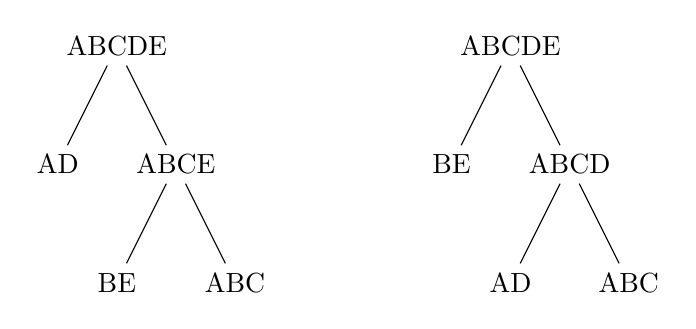
\begin{tikzpicture}
    \node (root1) at (0, 0) {ABCDE}
      child {node {AD}}
      child {node {ABCE}
        child {node {BE}}
        child {node {ABC}}};
    \node (root2) at (5, 0) {ABCDE}
      child {node {BE}}
      child {node {ABCD}
        child {node {AD}}
        child {node {ABC}}};
  \end{tikzpicture}
\end{frame}

\begin{frame}{Invalid decomposition trees}
  \centering
  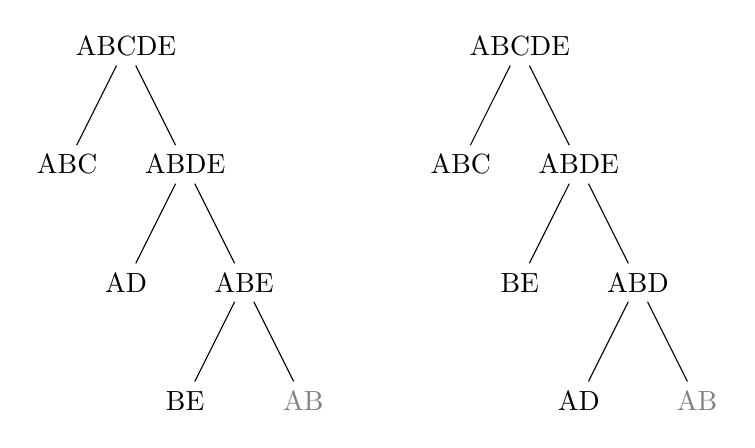
\begin{tikzpicture}
    \node (root1) at (0, 0) {ABCDE}
      child {node {ABC}}
      child {node {ABDE}
        child {node {AD}}
        child {node {ABE}
          child {node {BE}}
          child {node[gray] {AB}}}};
    \node (root2) at (5, 0) {ABCDE}
      child {node {ABC}}
      child {node {ABDE}
        child {node {BE}}
        child {node {ABD}
          child {node {AD}}
          child {node[gray] {AB}}}};
  \end{tikzpicture}

  \vspace{0.3cm}
  \small $R[AB]$ is not a consequence of a functional dependency.
\end{frame}

\begin{frame}{Change of observational unit}
  \begin{itemize}
    \item Traverse decomposition tree from bottom to top with joins
    \item After each join, perform summarization on new observational unit
    \item Example: student enrollment $\to$ student summary (avg.\ grade, total load)
    \item Order of joins and summarization is crucial
    \item Not trivial to calculate all possible decomposition trees
  \end{itemize}
\end{frame}

% ===========================================================================
\section{Data semantics and interpretation}
% ===========================================================================

\begin{frame}{Data semantics and interpretation}
  \begin{itemize}
    \item Beyond functional dependencies: \textbf{statistical dependencies}
    \item Attributes may exist in an unknown $P(A, B)$
    \item Important to understand relationships between observations:
      \begin{itemize}
        \item Independent? Identically distributed? Selection bias?
        \item Temporal dependence? Hidden variables?
      \end{itemize}
    \item Wrong assumptions $\to$ wrong conclusions
  \end{itemize}
\end{frame}

% ===========================================================================
\section{Unstructured data}
% ===========================================================================

\begin{frame}{Unstructured data}
  \begin{itemize}
    \item No predefined data model (text, images, videos)
    \item Can be converted to structured data (e.g., bag-of-words)
    \item Conversion is not always straightforward or lossless
    \item Out of scope of this book
  \end{itemize}
\end{frame}

% ---- Takeaways ----

\begin{frame}{Takeaways}
  \begin{itemize}
    \item The choice of observational unit is not always straightforward
    \item Format and types must reflect what the solution will ``see'' in
      production
    \item Normalization (storage) and tidy data (analysis) are complementary
    \item Tidiness is a matter of perspective
  \end{itemize}
\end{frame}

% ---- End ----

\begin{frame}[standout]
  Questions?
\end{frame}

\end{document}

\chapter{Data handling}
\label{chap:handling}
\glsresetall

\chapterprecishere{%
  $\dagger$ It's dangerous to go alone! Take this.
  \par\raggedleft--- \textup{Unnamed Old Man}, The Legend of Zelda}

In the previous chapter, I discussed the relationship between data format and data
semantics.  We also saw in \cref{chap:project} that data tasks --- specifically
integration and tidying --- must adjust the available data to reflect the kind of
input we expect in production.  Data handling consists of operating on this data.

For those tasks, we must be careful with the operations we perform on the data. At the
stage of data preparation, for example, we should never parametrize our data handling
pipeline in terms of information retrieved\footnote{For instance, imputation by the mean
of a column.} by the values of the data.  This is because such operations lead to \gls{leakage}
during evaluation and other biases in our conclusions.

In this chapter, we consider that tables are rectangular data structures in which values
of the same column share the same properties (i.e. the same type, same restrictions, etc.)
and each column has a name.  Moreover, we assume that any value is possibly
\emph{missing}.

From a mathematical definition of such tables, we can define a set of operations that can
be applied to them.  These operations are the building blocks of data handling pipelines:
combinations of operations that transform a dataset into another dataset.

Finally, I highlight some important properties of these operations.  Especially, the
split-invariance property, which ensures that the operations do not add bias to the data
due to the way the data was collected.

\begin{mainbox}{Chapter remarks}

  \boxsubtitle{Contents}

  \startcontents[chapters]
  \printcontents[chapters]{}{1}{}
  \vspace{1em}

  \boxsubtitle{Context}

  \begin{itemize}
    \itemsep0em
    \item Data handling consists of operating on tables.
    \item Properties of the operations are important to avoid bias.
    \item Data handling pipelines are a way to organize these operations.
  \end{itemize}

  \boxsubtitle{Objectives}

  \begin{itemize}
    \itemsep0em
    \item Define a formal structure for tables.
    \item Define a set of operations that can be applied to tables.
  \end{itemize}

  \boxsubtitle{Takeaways}

  \begin{itemize}
    \itemsep0em
    \item Split-invariant operations avoid sampling bias.
    \item One must understand the properties and premises of the operations.
  \end{itemize}
\end{mainbox}

{}
\clearpage

\section{Formal structured data}
\label{sec:formal-structured-data}

\newcommand{\domainof}[1]{\mathcal{D}\!\left(#1\right)}
\newcommand{\missing}{\text{?}}
\newcommand{\rowcard}[1][k_1, \dots, k_k]{\operatorname{card}\!\left(#1\right)}

In this section, I present a formal definition of structured data.  This definition is
compatible with the relational model and tidy data presented in \cref{chap:data}.
My definition takes into account the index\footnote{Also called grouping variables.} of
the table, which is a key concept in data handling.  We also consider that values can be
missing.  Repeated rows are represented by allowing cells to contain sets of values.
In this chapter, we consider dataset and table as synonyms.

\begin{defbox}{Indexed table}{itable}
An indexed table $T$ is a tuple $(K, H, c)$, where $K = \left\{K_i : i = 1, \dots,
k\right\}$ is the set of index columns, $H$ is the set of (non-index) columns, and $c :
\domainof{K_1} \times \dots \times \domainof{K_k} \times H \to \mathcal{V}$ is the cell function.
Here, $\mathcal{V}$ represents the space of all possible tuples of values, which
may include missing values $\missing$.  Values have arbitrary types, such as integers,
real numbers, strings, etc.
Each index column $K_i$ has a domain $\domainof{K_i}$, which is an enumerable set of
values.
\end{defbox}

A possible row $r$ of the table is indexed by a tuple $r = (k_1, \dots,
k_k)$, where $k_i \in \domainof{K_i}$.  Each row has a cardinality $\rowcard[r]$, which
represents how many times the entity represented by the row is present in the table.
A row $r$ with $\rowcard[r] = 0$ is considered to be missing.

A cell is then represented by a row $r$ and a column $h \in H$.  The value of the cell,
$\vec{v} = c(r, h)$ is a tuple of values in the domain $\domainof{h} \cup \{\missing\}$,
such that $|\vec{v}| = \rowcard[r]$.  We say that $\domainof{h}$ is the valid domain of
the column $h$.
The order of the elements in the tuple $\vec{v}$ is arbitrary but fixed.

\begin{defbox}{Nested row}{nested-row}
A \emph{nested
row} consists of a tuple of values that associates different columns with the same
repetition of the entity, i.e. \[
  \Big[ v^h_i : h \in H \Big]\text{,}
\]
where $c(r, h) = [v^h_i : i = 1, \dots, \rowcard[r]]$, assuming an arbitrary fixed order
of the columns $h$.
\end{defbox}

We can stack nested rows to form a matrix of values.  This matrix is called the value
matrix of the row $r$.

\begin{defbox}{Value matrix}{vmatrix}
The value matrix $V = (v_{i, j})$ of the row $r$ is \[
  \Big[ c(r, h) : h \in H \Big]\text{,}
\] with dimensions $\rowcard[r] \times |H|$.
\end{defbox}

We assume that value matrices --- and consequently row cardinalities --- are minimal. This
means that there are no nested rows $$v_{i, 1}, \dots, v_{i, |H|}$$ in the value matrices
such that $v_{i, j} = \missing$ for all $j$.

From these concepts, we can define the basic operations and properties that can be applied
to tables.

\subsection{Splitting and binding}

Split and bind are very basic operations that can be applied to tables.  They are
inverses of each other and are used to divide and combine tables, respectively.
They are important in the data science process because they play a key role in
data semantics and validation of solutions.

\begin{defbox}{Split operation}{split}
Given an indicator function $s : \domainof{K_1} \times \dots \times \domainof{K_k} \to
\left\{0, 1\right\}$, the split operation creates two tables, $T_0$ and $T_1$, that
contain only the rows for which
$s(r) = 0$ and $s(r) = 1$, respectively.

Mathematically, the split operation is defined as \[
  \operatorname{split}(T, s) = \left(T_0, T_1\right)\text{,}
\] where $T = (K, H, c)$, $T_i = (K, H, c_i)$, and \[
  c_i(r, h) = \begin{dcases}
    c(r, h) & \text{if } s(r) = i \\
    () & \text{otherwise.}
  \end{dcases}
\]
\end{defbox}

\emph{Note that, by definition, the split operation never ``breaks'' a row.  So, the
indices define the indivisible entities of the table.}  The resulting tables are
disjoint:

\begin{defbox}{Disjoint tables}{disjoint-tables}
  Two tables $T_0 = (K, H, c_0)$ and $T_1 = (K, H, c_1)$ are said to be disjoint if
  $$\rowcard[r; c_0] > 0 \Rightarrow \rowcard[r; c_1] = 0\text{ and}$$
  $$\rowcard[r; c_1] > 0 \Rightarrow \rowcard[r; c_0] = 0$$ for any $r$.
\end{defbox}

The binding operation is the inverse of the split operation.

\begin{defbox}{Bind operation}{bind}
  Given two disjoint tables
  $T_0 = (K, H, c_0)$ and $T_1 = (K, H, c_1)$, the binding operation creates a new table $T$
  that contains all the rows of $T_0$ and $T_1$.

  Mathematically, the binding operation is defined as \[
    \operatorname{bind}(T_0, T_1) = (K, H, c)\text{,}
  \] where $T_i = (K, H, c_i)$ and \[ c(r, h) = c_0(r, h) + c_1(r, h)\text{.} \]
  The operator $+$ stands for the tuple concatenation operator%
  \footnote{The order of the concatenation here is not an issue since we guarantee
  that at least one of the operands is empty.}.
\end{defbox}

\emph{Thus, a requirement for the binding operation is that the tables are disjoint in
terms of the row entities they have.}

\paragraph{Premises in real-world applications}

One important aspect of these functions is that we assume that the entities represented by
the rows are indivisible, and that any binding operation will never occur for tables that
share the same entities.

In real-world applications, this is not always true.  Many times, we do not know the
process someone else has used to collect the data.  In these cases, we must be careful
about the guarantees we discuss in this chapter.  On the other hand, one can consider the
premises we use as a guideline to design good data collection processes.

We can see data collection as the result of a splitting operation in the universe set of
all possible entities.  This is a good way to think about data collection, as we can try
to ensure that we collect all possible information about the entities we are interested
in.

This, of course, depends on what we define as the index columns of the table.  Consider
the example of collecting information about grades of students.  If we define the student's
name and year as the indexes, we must ensure that we collect all the grades of all
subjects a student has taken in a year.  We do not need, though, to collect information
from all students or all years.  On the other hand, if we define only the student's name
as the index column, we must collect all the grades of all subjects a student has taken
in all years.

In summary, the fewer variables we define as index columns, the more information we must
collect about each entity.  However, in the next sections, we show that assuming many index columns
leads to restrictions in the operations we can perform on the table.

This conceptual trade-off is important to understand when structuring the problem we are
trying to solve.  Neglecting these issues can lead to strong statistical biases and
incorrect conclusions.

\subsection{Split invariance}

One property we can study about data handling operations is whether they are distributive
over the bind operation.  This property is called \emph{split invariance}.

From now on, we will denote \[
  T_0 + T_1 = \operatorname{bind}(T_0, T_1)\text{,}
\] for any tables $T_0$ and $T_1$ to simplify the notation.

\begin{defbox}{Split invariance}{split-invariance}
An arbitrary data handling operation $f(T)$ is said to be split-invariant
if, for any table $T$ and split function $s$, the following equation holds \[
  f\!\left(T_0 + T_1\right) =
    f\!\left(T_0\right) + f\!\left(T_1\right)\text{,}
\] where $T_0, T_1 = \operatorname{split}\!\left(T; s\right)$.
\end{defbox}

Split invariance is a desirable property for data handling operations during the data
tasks described in \cref{chap:project}: integration and tidying.  Even while exploring
data, we should take effort to use split-invariant operations.

The reason is that split invariance ensures that the operation does not depend on the
split performed (usually unknown to us) to create the table we have in hand.  This
property is important to avoid \gls{leakage} or to bias the results of the
analysis\footnote{Note that split invariance is a sufficient but not necessary condition
for preventing leakage.  Split invariance provides not only a ``safe by default''
guarantee, but also a way to pinpoint possible sources of leakage.}.

\subsection{Illustrative example}

\begin{tablebox}[label=tab:grades1]{Data table of student grades.}
  \centering
  \rowcolors{2}{black!10!white}{}
  \begin{tabular}{cccc}
    \toprule
    \textbf{student} & \textbf{subject} & \textbf{year} & \textbf{grade} \\
    \midrule
    Alice & Chemistry & 2020 & 6 \\
    Alice & Math & 2019 & 8 \\
    Alice & Physics & 2019 & 7 \\
    Bob & Chemistry & 2018 & ? \\
    Bob & Chemistry & 2019 & 7 \\
    Bob & Math & 2019 & 9 \\
    Bob & Physics & 2019 & 4 \\
    Bob & Physics & 2020 & 8 \\
    Carol & Biology & 2020 & 8 \\
    Carol & Chemistry & 2020 & 3 \\
    Carol & Math & 2020 & 10 \\
    \bottomrule
  \end{tabular}
  \tcblower
  Data collected about student grades.  All information that is available is presented.
\end{tablebox}

Consider the example of data collected about student grades.  \Cref{tab:grades1}
exemplifies all information we can possibly have about the grades of students.  A missing
value in a cell of that table indicates that, for some reason, the information is not
retrievable.

The domains of the variables are:
\begin{itemize}
  \itemsep0em
  \item $\domainof{\text{student}} = \left\{\text{Alice}, \text{Bob}, \text{Carol}\right\}$;
  \item $\domainof{\text{subject}} = \left\{\text{Biology}, \text{Chemistry}, \text{Math},
    \text{Physics}\right\}$;
  \item $\domainof{\text{year}} = \mathbb{Z}$; and
  \item $\domainof{\text{grade}} = \left[0, 10\right]$.
\end{itemize}

Of course, in practice, we have no guarantee that the data we have is complete nor a
clear specification of the domain of the variables.  Instead, we must choose good
premises about the data we are working with.

Knowing that the data is complete, we can safely assume that:
\begin{enumerate}
  \itemsep0em
  \item Alice has never taken Biology;
  \item Bob passed Physics, although at the second attempt;
  \item Carol has only taken classes in 2020.
\end{enumerate}

\begin{tablebox}[label=tab:grades2]{Data table of student grades assuming student and subject as indices.}
  \centering
  \rowcolors{2}{black!10!white}{}
  \begin{tabular}{ccccc}
    \toprule
    \textbf{s} & \textbf{student} & \textbf{subject} & \textbf{year} & \textbf{grade} \\
    \midrule
    0 & Alice & Chemistry & (2020) & (6) \\
    1 & Alice & Math & (2019) & (8) \\
    1 & Alice & Physics & (2019) & (7) \\
    0 & Bob & Chemistry & (2018, 2019) & (?, 7) \\
    0 & Bob & Math & (2019) & (9) \\
    1 & Bob & Physics & (2019, 2020) & (4, 8) \\
    0 & Carol & Biology & (2020) & (8) \\
    0 & Carol & Chemistry & (2020) & (3) \\
    1 & Carol & Math & (2020) & (10) \\
    \bottomrule
  \end{tabular}
  \tcblower
  Indexed table with data from \cref{tab:grades1} assuming student and
  subject as indices.  The column $s$ is the split indicator.
\end{tablebox}

Now consider an arbitrary collection mechanism that considers student and subject as the
indices of the table.  \Cref{tab:grades2} shows the table we have in hand.  The column $s$
is the split indicator.  Only rows with $s = 1$ are available to us.

Now, about the statements we made before:
\begin{enumerate}
  \itemsep0em
  \item There is no way we can know if Alice has taken Biology or not.  It could be that
    the data collection mechanism failed to collect this information or that the
    information simply does not exist.
  \item We can safely assume that Bob has passed Physics in his second attempt, once all
    information about (Bob, Physics) is assumed to be available.
  \item There is no guarantee that Carol has only taken classes in 2020.  It could be that
    some row (Carol, subject) with a year different from 2020 is missing in the table.
\end{enumerate}

\begin{tablebox}[label=tab:grades3]{Data table of student grades assuming student as the index.}
  \centering
  \rowcolors{2}{black!10!white}{}
  \begin{tabular}{ccp{2.6cm}p{1.8cm}>{\raggedright\arraybackslash}p{1.2cm}}
    \toprule
    \textbf{s} & \textbf{student} & \textbf{subject} & \textbf{year} & \textbf{grade} \\
    \midrule
    1 & Alice & (Chemistry, Math, Physics) & (2020, 2019, 2019) & (6, 8, 7) \\
    0 & Bob & (Chemistry, Chemistry, Math, Physics, Physics) & (2018, 2019, 2019, 2019, 2020) & (?, 7, 9, 4, 8) \\
    1 & Carol & (Biology, Chemistry, Math) & (2020, 2020, 2020) & (8, 3, 10) \\
    \bottomrule
  \end{tabular}
  \tcblower
  Indexed table with data from \cref{tab:grades1} assuming student
  as index.  The column $s$ is the split indicator and only rows with $s = 1$ are available to us.
\end{tablebox}

Now consider an arbitrary collection mechanism that considers student as the index of the table.
Imposing this restriction would difficult the data collection process, but it would
guarantee that we have all information about each student.  \Cref{tab:grades3} shows the
table we have in hand.  As before, the column $s$ is the split indicator and only rows with
$s = 1$ are available to us.

Our conclusions may change again:
\begin{enumerate}
  \itemsep0em
  \item We can safely assume that Alice has never taken the Biology class, as $\text{Biology}
    \not\in c(\text{Alice}, \text{subject})$.
  \item There is no information about Bob's grades, so we can not affirm nor deny anything
    about his grades.
  \item We can safely assume that Carol has only taken classes in 2020, as $c(\text{Carol},
    \text{year})$ contains only values with 2020.
\end{enumerate}

It is straightforward to see that the fewer index columns we have, the more information we
have about the present entities.  Also, it is clear how important the assumptions on the
index columns are to the conclusions we can draw from the data. Consequently,
split-invariant operations can preserve valid conclusions about the data even when
information is missing\footnote{Absence can be due to incomplete data collection or
artificial splitting for validation; consult \cref{chap:planning}.}.

\section{Data handling pipelines}

In the literature and in software documentation, you will find a variety of terms used to
describe data handling operations\footnote{%
  The terminology ``data handling'' itself is not universal.  Some authors and libraries
  call it ``data manipulation'', ``data wrangling'', ``data shaping'', or ``data
  engineering''.  I use the term ``data handling'' because it seems more generic.
  Also, it avoids confusion with the term ``data
  manipulation'' which has a negative connotation in some contexts.}. %
They often refer to the same or similar operations, but the terminology can be confusing.
In this section, I present a summary of these operations mostly based on
\textcite{Wickham2023} definitions\footnote{Which they call \emph{verbs}.}.


During the preparation of data for our project, we will need to perform a set of operations
on possibly multiple datasets.  These operations are organized in a pipeline, where the
outputs of one operation are the inputs of the next one.
Operations are extensively parameterized, for instance, most of them can use predicates to
define the groups, arrangements, or conditions under which they should be applied.

\begin{figurebox}[label=fig:pipeline]{Example of data handling pipeline.}
  \centering
  \begin{tikzpicture}[every node/.style={font=\small, inner sep=4pt}]
    \node (s1) [darkcircle] at (0, 0) {Source 1};
    \node (s2) [darkcircle] at (0, -2) {Source 2};
    \node (f1) [mediumblock] at (2, 0) {$f_1$};
    \node (f2) [mediumblock] at (4, 0) {$f_2$};
    \node (f3) [mediumblock] at (2, -2) {$f_3$};
    \node (f4) [mediumblock] at (4, -2) {$f_4$};
    \node (f5) [mediumblock] at (6, -1) {$f_5$};
    \node (data) [darkcircle, minimum width=15mm] (data) at (8, -1) {Data};

    \path [line] (s1) -- (f1);
    \path [line] (f1) -- (f2);
    \path [line] (f1.east) -- (f4);
    \path [line] (s2) -- (f3);
    \path [line] (f3) -- (f4);
    \path [line] (f2) -- (f5);
    \path [line] (f4) -- (f5);
    \path [line] (f5) -- (data);
  \end{tikzpicture}
  \tcblower
  A data handling pipeline is a set of operations that transform a dataset into
  another dataset.  We can have more than one source dataset and the output is a single
  dataset where each row represents a sample in the observational unit we are interested
  in.
\end{figurebox}

In \cref{fig:pipeline}, we show an example of a data handling pipeline.  The pipeline
starts with two source datasets, Source 1 and Source 2.  The datasets are processed by a
set of operations, $f_1, f_2, f_3, f_4, f_5$, and the output is a single dataset,
Data.  Our goal at the data tasks --- see \cref{sub:workflow} --- is to create a dataset
that is representative of the observational unit we are interested in.  Representative
here means that the dataset is tidy\footnote{Remember that our definition of tidiness
depends on the observational unit.  That means, in practice, that if the original data
sources are in a observational unit different from the one we are interested in, after
joining them, the connecting variables may need to be removed to eliminate transitive
dependencies.  Consult \cref{sub:tidy-not-tidy,sub:change-unit}.} and that the priors,
i.e. the distribution of the data is faithful to the real distribution of the phenomenon.

A pipeline is more flexible than a chain of operations because it can handle more complex
structures, where different branches (forks) of processing occur simultaneously, and then
come together (merges) later in the workflow.  For instance, the output of $f_1$ is the
input of $f_2$ and $f_4$ (fork), and $f_5$ has as input the outputs of $f_2$ and $f_4$
(merge).

Pipelines are great conceptual tools to organize the data handling process.  They allow
for the separation of concerns, where each operation is responsible for a single task.
Also, declaring the whole pipeline at once allows for the optimization of the operations
and the use of parallel processing.  This is important when dealing with large datasets.
The declarative approach, as opposed to the imperative one, makes it easier to reason about
and maintain the code\footnote{Tidyverse and Polars are examples of
libraries that use a declarative approach to data handling.}.

\section{Split-invariant operations}
\label{sec:split-invariant-ops}

In this section, I present a set of operations that are split-invariant.  One can safely
apply these operations to the data without worrying about biasing the dataset.

For each operation, we discuss its application on some tidying issues presented in
\cref{sub:messy}.  The issues I address here\footnote{%
The issue of multiple types of observational units stored in the same table is better
dealt with by database normalization.  More on this subject is discussed in
\cref{sub:projection}.}:
\begin{itemize}
  \itemsep0em
  \item Headers are values, not variable names;
  \item Multiple variables are stored in one column; % [mutate/select problem]
  \item Variables are stored in both rows and columns;
  \item A single observational unit is stored in multiple tables.
\end{itemize}



\subsection{Tagged splitting and binding}

We saw that one trivial, yet important, operation is to bind datasets.  This is the
process of combining two or more datasets into a single dataset.  To make the
operation reversible, we can parametrize it with a split column that indicates the source
of each row.

\begin{defbox}{Tagged bind operation}{tagged-bind}
  Given two or more disjoint tables $T_i = (K, H, c_i)$, $i = 0, 1, \dots$, the tagged
  bind operation creates a new table $T = (K, H \cup \{s\}, c)$ that contains all the rows
  of tables $T_i$.  The split column $s$ is a new column that indicates the source of each
  row.

  Mathematically, the tagged bind operation is defined as \[
    \operatorname{bind}_{s}(T_0, T_1, \dots) = T\text{,}
  \] where $c(r, h) = c_0(r, h) + c_1(r, h) + \dots$ if $h \in H$ and \[
    c(r, s) = \left[ i \right]^{d} \text{,}
  \]
  where $i$ is the index of the table $T_i$ that contains the row $r$, i.e. $d =
  \rowcard[r; c_i] > 0$.
\end{defbox}

When binding datasets by rows, the datasets must have the same columns.  In practice,
one can assume, if a column is missing, that all values in that column are missing.

The indication of the source table usually captures some hidden semantics that has split
the tables in the first place. For instance, if each table represents data collected in a
different year, one can create a new column \emph{year} that contains the year of the
data.  It is important to pay attention to the semantics of the split column, as it can
also contain extra information.

\begin{tablebox}[label=tab:gas-usage]{Gas usage datasets.}
  \centering
  \rowcolors{2}{black!10!white}{}
  \begin{tabular}{ccc}
    \toprule
    \textbf{month} & \textbf{gas} & \textbf{distance} \\
    \midrule
    1 & 48.7 & 1170 \\
    2 & 36.7 & 1100 \\
    3 & 37.8 & 970 \\
    \dots & \dots & \dots \\
    \bottomrule
  \end{tabular}
  ~
  \rowcolors{2}{black!10!white}{}
  \begin{tabular}{ccc}
    \toprule
    \textbf{month} & \textbf{gas} & \textbf{distance} \\
    \midrule
    1 & 143.7 & 1470 \\
    2 & 156.7 & 1700 \\
    3 & 170.8 & 1870 \\
    \dots & \dots & \dots \\
    \bottomrule
  \end{tabular}
  \tcblower
  Monthly gas usage data from US (left) and Brazil (right) residents.
\end{tablebox}

Consider \cref{tab:gas-usage}, which contains monthly gas usage data from
US and Brazil residents.  From the requirements described in the previous section, we can
safely bind these datasets --- as they are disjoint.  We can use as a tag a new column to
represent the country.  However, an attentive reader will notice that the unit of
measurement of the gas usage and distance are different in each table: gallons and miles
in the US dataset and liters and kilometers in the Brazil dataset.  Ideally, thus, we
should create two other columns to represent the units of measurement.

It is straightforward to see that this operation solves the issue of a single
observational unit being stored in multiple tables described in \cref{sub:messy}.

The reverse function consists of splitting the dataset using as a predicate the split column.

\begin{defbox}{Tagged split operation}{tagged-split}
  Let $s$ be a non-index column of a table $T = (K, H \cup \{s\}, c)$ with $\domainof{s}$
  known and finite, and such that $c(r, s)$ contains only unique values. The tagged split
  operation parametrized by $s$ creates disjoint tables $T_i = (K, H, c_i)$ that contain
  only the rows $r$ for which $c(r, s) = i$.

  Mathematically, the tagged split operation is defined as \[
    \operatorname{split}_{s}(T) = \left(T_0, T_1, \dots\right)\text{,}
  \] where $c_i(r, h) = c(r, h)$ if $i \in c(r, s)$ and $c_i(r, h) = ()$ otherwise.
\end{defbox}

Note that the tagged split is split-invariant by definition, since we assume that the
nested rows of the input table $T$ contain only one value for column $s$ for all
rows\footnote{We consider a slightly different definition of split invariance here, where
the binding operation is applied to each element of the output of the split operation.}.
Failing to meet this assumption can lead to a biased split.  Also, in practice, it is
good practice to keep the column $s$ in the output tables to preserve information about
the source of the rows.  In terms of storage, smart strategies can be used to avoid the
unnecessary repetition of the same value in column $s$.

\subsection{Pivoting}

Another important operation is pivoting datasets.  There are two types of pivoting:
long-to-wide and wide-to-long.  These operations are reversible and are the inverse
of each other.

Pivoting long-to-wide requires a name column --- whose discrete and finite
possible values will become the names of the new columns --- and a value column --- whose
values will be \emph{spread} across the rows.  Other than these columns, all remaining columns
must be indexes.

\begin{defbox}{Pivot long-to-wide operation}{pivot-l2w}
  Let $T = (K \cup \{\text{name}\}, \{\text{value}\}, c)$. The pivot long-to-wide
  operation is defined as \[
    \operatorname{pivot}_\text{name}(T) = T'\text{,}
  \] where $T' = (K, \domainof{\text{name}}, c')$ and \[
    c'(r, h) = c\left(r + (h),~\text{value}\right)\text{,}
  \]
  for all valid row $r$ and $h \in \domainof{\text{name}}$.
\end{defbox}

Note however that the operation only works if $\rowcard[r + (h); c]$ is constant for all
$h \in \domainof{\text{name}}$.  If this is not the case, one must aggregate the rows
before applying the pivot operation.  This is discussed in \cref{sub:aggregation}.

Pivoting wide-to-long\footnote{Also known as unpivot.} is the reverse operation. One must
specify all the columns whose names are the values of the previously called ``name column.''
The values of these columns will be \emph{gathered} into a new column. As before, all
remaining columns are indexes.

\begin{defbox}{Pivot wide-to-long operation}{pivot-w2l}
  Let $T = (K, H, c)$ be a table.  The pivot wide-to-long
  operation is defined as \[
    \operatorname{pivot}^{-1}(T) = T'\text{,}
  \] where $T' = (K \cup \{\text{name}\}, \{\text{value}\}, c')$, $\domainof{\text{name}}
  = H$ and \[
    c'((r, h), \text{value}) = c(r, h)\text{,}
  \] for all valid row $r$ and $h \in H$.
\end{defbox}

In practical applications, where not all remaining columns are indexes, one must aggregate
rows or drop extra non-indexed columns beforehand.  This is discussed in
\cref{sub:aggregation,sub:selection}.

\begin{tablebox}[label=tab:pivot]{Pivoting example.}
    \centering
    \rowcolors{2}{black!10!white}{}
    \begin{tabular}{ccc}
      \toprule
      \textbf{city} & \textbf{year} & \textbf{qty.} \\
      \midrule
      A & 2019 & 1 \\
      A & 2020 & 2 \\
      A & 2021 & 3 \\
      B & 2019 & 4 \\
      B & 2020 & 5 \\
      B & 2021 & 6 \\
      \bottomrule
    \end{tabular}
    ~
    \rowcolors{2}{black!10!white}{}
    \begin{tabular}{cccc}
      \toprule
      \textbf{city} & \textbf{2019} & \textbf{2020} & \textbf{2021} \\
      \midrule
      A & 1 & 2 & 3 \\
      B & 4 & 5 & 6 \\
      \bottomrule
    \end{tabular}
  \tcblower
  The left-hand-side table is in the long format and the right-hand-side table is in the
  wide format.
\end{tablebox}

\Cref{tab:pivot} shows an example of pivoting.  Here, we can consider \emph{city} and
\emph{year} as the index columns.  The left-hand-side table is in the long format and the
right-hand-side table is in the wide format.  Using the pivot long-to-wide operation with
\emph{year} as the name column and \emph{qty.} as the value column, we can obtain the
right-hand-side table.  The reverse operation will give us the left-hand-side table.

To show that the pivot operation is split-invariant, one can see that, given
$T_0 = (K, H, c_0)$ and $T_1 = (K, H, c_1)$ disjoint tables,
\[
  \operatorname{pivot}_\text{name}\!\left(T_0\right) + \operatorname{pivot}_\text{name}\!\left(T_1\right) = \\
    (K, \domainof{\text{name}}, c_0') + (K, \domainof{\text{name}}, c_1')\text{,}
\] where $c_i'(r, h) = c_i(r + (h), \text{value})$.  However, by the disjoint property of
the tables, we have that \[
  c_0(r + (h), \text{value}) + c_1(r + (h), \text{value}) = c(r + (h), \text{value})\text{,}
\] for the table $T = (K, H, c) = T_0 + T_1$. So,
\begin{multline*}
  (K, \domainof{\text{name}}, c_0') + (K, \domainof{\text{name}}, c_1') =
    (K, \domainof{\text{name}}, c') =\\
    \operatorname{pivot}_\text{name}\!\left(T\right)\text{,}
\end{multline*}
where $c'(r, h) = c(r + (h), \text{value})$.

Similarly, the reverse operation is also split-invariant.

Using the pivot operation, we can solve the issues of headers being values, not variable
names and variables being stored in both rows and columns.  In the first case, we can pivot
the table to have the headers as the domain of a new index (name column).  In the second
case, we have to pivot both long-to-wide and wide-to-long to solve the issue.

\subsection{Joining}

Joining is the process of combining two datasets into a single dataset based on common
columns.  This is one of the two fundamental operations in relational algebra. We will see
the conditions under which the operation is split invariant. However, the join operation
has some other risks you should be aware of; consult \cref{sec:normalization} for more
details.

Adapting the definitions of join in our context, we can define it as follows.
For the sake of simplicity, we denote $r[U]$ as the row $r$ restricted to the index
columns in $U$, i.e.
\begin{equation*}
  % \label{eq:row-subscript}
  r[U] = (k_i : k_i \in \domainof{K_i} \forall K_i \in U)\text{.}
\end{equation*}

\begin{defbox}{Join operation}{join}
  Let $T' = (K', H', c')$ and $T'' = (K'', H'', c'')$ be two tables such that $K'
  \cap K'' \neq \emptyset$ and $H' \cap H'' = \emptyset$.  The join operation is
  defined as \[
    \operatorname{join}(T', T'') = T\text{,}
  \] where $T = (K' \cup K'', H' \cup H'', c)$ and \[
    c(r, h) = ()
  \] if $\rowcard[{r[K']; c'}] = 0$ or $\rowcard[{r[K'']; c''}] = 0$, for all $h$.
  Otherwise: \[
    c(r, h) = \begin{dcases}
      c'(r[K'], h) & \text{if } h \in H'\text{,} \\
      c''(r[K''], h) & \text{if } h \in H''\text{.}
    \end{dcases}
  \]
\end{defbox}

The join of two tables is the operation that returns a new table with the columns of both
tables.  Let $U$ be the common set of index columns.  For each occurring value of $U$ in
the first table, the operation will look for the same value in the second table.  If it
finds it, it will create a new row with the columns of both tables.  If it does not find
it, no row will be created.

Note that, like in pivoting long-to-wide, one must ensure that the cardinality of the
joined rows is constant for all $h \in H' \cup H''$.  If this is not the case, one must
aggregate the rows before applying the join operation.  This is discussed in
\cref{sub:aggregation}.

Before we discuss whether the join operation is split-invariant\footnote{Note that up to
this point, we have defined this property only for unary operations.}, we can discuss a
variation of the join operation: the left join.  The left join is the same as the join
operation, but if the value of $U$ is missing in the second table, the operation will
create a new row with the columns of the first table and missing values for the columns of
the second table.

In our context, this operation is a unary operation, where the second table is
a fixed parameter.

\begin{defbox}{Left join operation}{left-join}
  Let $T' = (K', H', c')$ and $T'' = (K'', H'', c'')$ be two tables such that $K'
  \cap K'' \neq \emptyset$ and $H' \cap H'' = \emptyset$.  The left join operation is
  defined as \[
    \operatorname{join}(T'; T'') = \operatorname{join}_{T''}(T') = T\text{,}
  \] where $T = (K' \cup K'', H' \cup H'', c)$ and \[
    c(r, h) = ()
  \] if $\rowcard[{r[K']; c'}] = 0$ for all $h$. Otherwise:
  \[
    c(r, h) = \begin{dcases}
      c'(r[K'], h) & \text{if } h \in H'\text{,} \\
      c''(r[K''], h) & \text{if } h \in H''\text{.}
    \end{dcases}
  \]
\end{defbox}

The left join operation is split-invariant.  To see this, consider two disjoint tables
$T_0 = (K, H, c_0)$ and $T_1 = (K, H, c_1)$, and a third table $T' = (K', H', c')$ such
that $K \cap K' \neq \emptyset$ and $H \cap H' = \emptyset$.  We have that
\begin{multline*}
  \operatorname{join}_{T'}(T_0) + \operatorname{join}_{T'}(T_1) =
  T_0' + T_1' =\\
    (K \cup K', H \cup H', c_0') + (K \cup K', H \cup H', c_1')\text{,}
\end{multline*}
where the meaning of each term is clear from the \cref{def:left-join}.
It is straightforward to see that rows in $T_0'$ and $T_1'$ are disjoint, since at least
part of the indices in $K \cup K'$ are different between them.

Moreover, \[
  \operatorname{join}_{T'}(T_0 + T_1) = (K \cup K', H \cup H', c')
\] with $c'(r, h) = ()$ only if both $\rowcard[{r[K]; c_0}] = 0$ and $\rowcard[{r[K];
c_1}] = 0$.  Otherwise, $c'(r, h) = c_0(r[K], h) + c_1(r[K], h)$ if $h \in H$ and $c'(r,
h) = c_0(r[K], h)$ if $h \in H'$.

Thus, \[
  \operatorname{join}_{T'}(T_0 + T_1) = \operatorname{join}_{T'}(T_0) + \operatorname{join}_{T'}(T_1)\text{.}
\]

Our conclusion is that the left join operation given a fixed table is split-invariant.
So we can safely use it to join tables without worrying about biasing the dataset once we
fix the second table.

I conjecture that the (inner) join operation shares similar properties but it is not as
safe; nonetheless, a clear definition of split invariance for binary operations is needed.
This is left as a thought exercise for the reader.  Notice that the traditional join has
the ability to ``erase'' rows from any of the tables involved in the operation.  This is a
potential source of bias in the data.  This further emphasizes the importance of
understanding the semantics of the data schema before joining tables --- consult
\cref{sec:normalization}.

\subsection{Selecting}
\label{sub:selection}

Selecting is the process of choosing a subset of non-index columns from a dataset.  The
remaining columns are discarded.  Rows of the table remain unchanged.

Although very simple, the selection operation is useful for removing columns that are not
relevant to the analysis.  Also, it might be needed before other operations, such as
pivoting, to avoid unnecessary columns (wide-to-long) and to keep only the value column
(long-to-wide).

\begin{defbox}{Selection operation}{selection}
  Let $T = (K, H, c)$ be a table and $H' \subseteq H$.  The selection operation is
  defined as \[
    \operatorname{select}_{H'}(T) = T'\text{,}
  \] where $T' = (K, H', c)$.
\end{defbox}

Sometimes, it is useful to select columns based on a function of the column properties.
In other words, the selection operation can be parameterized by a predicate.  The predicate
is a function that returns a logical value given the column.

\begin{defbox}{Predicate selection operation}{predicate-selection}
  Let $T = (K, H, c)$ be a table and $P : H \to \{0, 1\}$ be a predicate.  The predicate
  selection operation is defined as \[
    \operatorname{select}_{P}(T) = T'\text{,}
  \] where $T' = (K, H', c)$ and $H' = \{h \in H : P(h) = 1\}$.
\end{defbox}

It is trivial to see that, if $P$ does not depend on the values of the columns (i.e., has no
access to $c$), the predicate selection operation is split-invariant.  This is because the
operation does not change the rows of the table nor does it depend on the values of the rows.

One example of the use of the predicate selection operation is to keep columns whose
values are in a specific domain.  For instance, to keep only columns that contain real
numbers, we choose $P(h) = 1$ if $\domainof{h} = \mathbb{R}$, and $P(h) = 0$ otherwise.

The case where the predicate depends on the values of the columns is discussed in
\cref{sub:grouped-arranged}.

\subsection{Filtering}
\label{sub:filtering}

Filtering is the process of selecting a subset of rows from a dataset based on a
predicate.

A predicate can be a combination of other predicates using logical operators, such as
logical disjunction (or) or logical conjunction (and).  In the general case, predicates
need to be robust enough to deal with value matrices of any size and those that contain missing
values.

After filtering, the dataset will contain only the rows that satisfy the predicate.
Columns remain unchanged.

In its simplest form, we can assume that $\rowcard[r] \leq 1$ for all $r$ and that the
predicates are applied to each row independently.  In this case, the value matrix $V(r)$
is just a tuple with a single value for each non-index column.

Without loss of generality, we can assume that predicates are combined using logical
disjunction (or)\footnote{The reason is that sequential application of filtering is
equivalent to combining the predicates using logical conjunction (and).}.

For instance, the predicate \code{age > 18} will select all rows where the value in the
age column is greater than 18.  Keeping each row independent, we can also generalize
predicates to deal with the values of the indexes as well.

\begin{defbox}{Filtering operation}{filtering}
  Let $T = (K, H, c)$ be a table and $P_1, \dots P_n$ be predicates.  The
  filtering operation is defined as \[
    \operatorname{filter}_{P_1, \dots, P_n}(T) = T'\text{,}
  \] where $T' = (K, H, c')$ and \[
    c'(r, h) = \begin{dcases}
      c(r, h) & \text{if } \bigvee_{i = 1}^{n} P_i(r, V(r)) = 1\text{,} \\
      () & \text{otherwise}\text{,}
    \end{dcases}
  \] where predicate $$P_i : \bigtimes_{K_i} K_i \times
  \bigtimes_{h\in H}\left(\domainof{h} \cup \{?\}\right) \to \{0, 1\}$$ is applied to the value
  matrix $V(r)$ of the row $r$.
\end{defbox}

It is also trivial to see that the filtering operation is split-invariant, even in its
generalized form where the value matrix has many rows.  This property comes from the fact
that rows are treated independently.  More complex cases are discussed in
\cref{sub:grouped-arranged}.

\subsection{Mutating}

Mutating is the process of creating new columns in a table.  The operation is reversible,
as the original columns are kept.  The new columns are added to the dataset.

The values in the new column are determined by a function of the rows.  The expression is
a function that returns a vector of values given the values in the other columns.
Similarly to filtering, in its simplest form, we can assume that $\rowcard[r] \leq 1$ for
all $r$ and that the predicates are applied to each row independently.

\begin{defbox}{Mutation operation}{mutating}
  Let $T = (K, H, c)$ be a table and $f$ be a transformation function.  The mutating
  operation is defined as \[
    \operatorname{mutate}_{f}(T) = T'\text{,}
  \] where $T' = (K, H \cup \{ h' \}, c')$ and \[
    c'(r, h) = \begin{dcases}
      c(r, h) & \text{if } h \in H\text{,} \\
      f(r, V(r)) & \text{if } h = h'\text{,}
    \end{dcases}
  \] where the function $$f : \bigtimes_{K_i \in K} K_i \times \bigtimes_{h\in H}
  \left(\domainof{h} \cup \{?\}\right) \to \domainof{h'} \cup \{?\}$$ is applied to the
  value matrix $V(r)$ of the row $r$.
\end{defbox}

The expression can be a simple function, such as \code{y = x + 1}, or a more complex
function, such as
\begin{center}
  \code{y = ifelse(x > 0, 1, 0)}.
\end{center}
Here, x and y are the names of an existing and the new column, respectively. The
\code{ifelse(a, b, c)} function is a conditional function that returns 1 if the condition
is true and 0 otherwise.

This function solves the issue of multiple variables stored in one column described in
\cref{sub:messy}.

As with filtering, the mutating operation is split-invariant even if $\rowcard[r] > 1$ for
any $r$\footnote{It just changes the input space of function $f$.}.  This is because the
operation is applied to each row independently.  In this general case, an extra
requirement is that the function $f$ must return tuples with the same cardinality as
the row it is applied to.

\subsection{Aggregating}
\label{sub:aggregation}

Many times, it is easier to reason about the table when all rows have cardinality 1.
Aggregation ensures that the table has this property.

\begin{defbox}{Aggregation operation}{aggregating}
  Let $T = (K, H, c)$ be a table and $f$ be an aggregation function.  The aggregation
  operation is defined as \[
    \operatorname{aggregate}_{f}(T) = T'\text{,}
  \] where $T' = (K, H, c')$ and \[
    c'(r, h) = f(r, V(r))[h]\text{,}
  \] where function $f$ is applied to the value matrix $V(r)$ of the row $r$ and it has
  an image $$\left(\domainof{h} \cup \{?\} : h \in H\right)\text{,}$$ independently of the
  input size.  The notation $v[h]$ refers to the value corresponding to the column $h$ in the
  output tuple.
\end{defbox}

As with mutation, aggregation is split-invariant as it treats each row independently,
even if the function $f$ considers order semantics of the values in the matrix.

\subsection{Ungrouping}
\label{sub:ungrouping}

We discussed that the fewer index columns a table has ---
assuming we guarantee that all information about that entity is present --- the safer
it is to infer conclusions from the data.  Thus, reducing the number of indices
must be done very carefully --- more on that in \cref{sub:projection}.

On the other hand, sometimes it is useful to increase the number of index columns.  For
instance, pivoting long-to-wide requires all columns except one to be indexes.  The
operation that transforms some of the columns in the table into indexes is called ungrouping.
The reason for the name is that the operation decreases the cardinality of rows
by creating new rows, effectively ungrouping the values.

\begin{defbox}{Ungrouping operation}{grouping}
  Let $T = (K, H, c)$ be a table and $h' \in H$ such that $\domainof{h'}$ is known and
  finite.  The ungrouping operation is defined as \[
    \operatorname{ungroup}_{h'}(T) = T'\text{,}
  \] where $T' = (K \cup \{h'\}, H \setminus \{h'\}, c')$, and \[
    c'(r + r', h) = (v_{i,h} : i)\text{,}
  \] where $r$ refers to values of the indices in $K$, $r'$ refers to the value of the new index
  $h'$, and $v_{i,h}$ is the value of the column $h$ in any $i$-th nested row of the value
  matrix $V(r; T)$ in the original table such that \[
    v_{i, h'} = r'\text{.}
  \]
\end{defbox}

Note that the operation requires that the column $h'$ has no missing values.

\begin{tablebox}[label=tab:ungroup]{Ungrouping example.}
  \centering
  \rowcolors{2}{black!10!white}{}
  \begin{tabular}{ccc}
    \toprule
    \textbf{city} & \textbf{year} & \textbf{qty.} \\
    \midrule
    A & (2019, 2020, 2020, 2021) & (1, 2, 3, 4) \\
    B & (2019, 2020, 2021) & (5, 6, 7) \\
    \bottomrule
  \end{tabular}

  \vspace{1em}
  \rowcolors{2}{black!10!white}{}
  \begin{tabular}{ccc}
    \toprule
    \textbf{city} & \textbf{year} & \textbf{qty.} \\
    \midrule
    A & 2019 & 1 \\
    A & 2020 & (2, 3) \\
    A & 2021 & 4 \\
    B & 2019 & 5 \\
    B & 2020 & 6 \\
    B & 2021 & 7 \\
    \bottomrule
  \end{tabular}
  \tcblower
  The index of the top table is the column \emph{city}.  The bottom table is the result of
  ungrouping the column \emph{year}.
\end{tablebox}

\Cref{tab:ungroup} shows an example of ungrouping.  In the top table, there are two rows,
one with cardinality 4 and the other with cardinality 3.  The column \emph{year} is
ungrouped, creating new rows for each value in the nested row.  The bottom table is the
result of ungrouping the column \emph{year}.  Although there were 7 nested rows in the
original table, the bottom table has 6 rows --- the number of nested rows is preserved
however.  The reason is that the row (A, 2020) has cardinality 2.

The ungrouping operation is split-invariant.  To see this, consider two disjoint tables
$T_0 = (K, H, c_0)$ and $T_1 = (K, H, c_1)$, we have
\begin{multline*}
  \operatorname{ungroup}_{h'}(T_0) + \operatorname{ungroup}_{h'}(T_1) = \\
    \left(K \cup \{h'\}, H \setminus \{h'\}, c_0'\right) +
    \left(K \cup \{h'\}, H \setminus \{h'\}, c_1'\right)\text{,}
\end{multline*}
where $c_j'(r + r', h) = (v_{i,h} : i \text{ such that } v_{i, h'} = r')$. Since the
tables are disjoint, the rows of the output tables are also disjoint.  In other words,
For any $r$, either $\rowcard[{r + r'; c_0}] = 0$ or $\rowcard[{r + r'; c_1}] = 0$
independently of the value of $r'$.  The reason is that there is no possible $v_{i,h'} =
r'$ if $r$ is not present in the table.

Then,
\begin{multline*}
  \left(K \cup \{h'\}, H \setminus \{h'\}, c_0'\right) +
  \left(K \cup \{h'\}, H \setminus \{h'\}, c_1'\right) = \\
    \left(K \cup \{h'\}, H \setminus \{h'\}, c'\right)\text{,}
\end{multline*}
where $c'(r + r', h) = c_0'(r + r', h) + c_1'(r + r', h)$.

\section{Other operations}

We saw that, under reasonable premises, split-invariant operations are safe to use in the
context of tidying and data integration.  However, data handling does not happen only in
the context of tidying and integrating datasets\footnote{And, sometimes, we may need to
use other transformations even for these tasks.}.  It is also used in tasks like data
exploration and data preprocessing.  In these cases, other operations are needed.

In this section, we discuss some of these operations.  Instead of focusing on the
mathematical definitions, we will discuss the semantics of the operations and some
of their properties.

\subsection{Projecting or grouping}
\label{sub:projection}

Projection is one of the two fundamental operations in relational algebra --- consult
\cref{sec:normalization} for more details.  In database normalization theory, tables ---
called relations --- are slightly different from the tables we are discussing here. The
major difference is that they are sets of tuples, which means that each tuple is unique.
In our scenario, this is similar to what we call rows represented by the possible values
of the index columns of the table.

Adapting the definitions of projection to our context, we can define it as follows.

\begin{defbox}{Projection operation}{projection}
  Let $T = (K, H, c)$ be a table and $K' \subset K$ a subset of the columns.  The
  projection operation is defined as \[
    \operatorname{project}_{K'}(T) = T'\text{,}
  \] where $T' = (K', H \cup (K \setminus K'), c')$ and \[
    c'(r, h) = \begin{dcases}
      \sum_{r'} c(r + r', h) & \text{if } h \in H \\
      \sum_{k' \in \domainof{h}} k' & \text{if } h \in K \setminus K'\text{,}
    \end{dcases}
  \] for all valid row $r$ considering the indices $K'$ and for all tuples $r' = (k_i :
  i)$ such that $k_i \in \domainof{K_i}$ for all $K_i \in K \setminus K'$.
\end{defbox}

We can see that projection for our tables is a little more complex than the usual
projection in relational algebra.  Consider the example we discussed in
\cref{sec:normalization} as well, where we have a table with the columns \emph{student},
\emph{subject}, \emph{year}, and \emph{grade}.

\begin{tablebox}[label=tab:student-grade-handling]{Student grade table.}
  \centering
  \rowcolors{2}{black!10!white}{}
  \begin{tabular}{cccc}
    \toprule
    \textbf{student} & \textbf{course} & \textbf{course credits} & \textbf{grade} \\
    \midrule
    Alice & Math & 4 & A \\
    Alice & Physics & 3 & B \\
    Bob & Math & 4 & B \\
    Bob & Physics & 3 & A \\
    Carol & Math & 4 & C \\
    \bottomrule
  \end{tabular}

  \vspace{1em}
  \rowcolors{2}{black!10!white}{}
  \begin{tabular}{cccc}
    \toprule
    \textbf{course} & \textbf{student} & \textbf{course credits} & \textbf{grade} \\
    \midrule
    Math & (Alice, Bob, Carol) & (4, 4, 4) & (A, B, C) \\
    Physics & (Alice, Bob, Carol) & (3, 3, ?) & (B, A, ?) \\
    \bottomrule
  \end{tabular}
  \tcblower
  (Top) An example of a table of students and their grades in courses.  The columns
  \emph{student} and \emph{course} are the index columns. (Bottom) The same table
  projected into the entity \emph{course}.
\end{tablebox}

\Cref{tab:student-grade-handling} (top) shows that table adapted for our definitions.
Suppose we want to project the table to have only the entity \emph{course}.
Now each row (bottom table) represents a course.  The column \emph{student} is not an
index column anymore, and the values in the column are exhaustive and unique, i.e.,
the whole set $\domainof{\text{student}}$ is represented in the column for each row.

Thus, projection is a very useful operation when we want to change the observational unit
of the data, particularly to the entity represented by a subset of the index columns.
Semantically, projection groups the rows by the values.

It is easy to see that the projection operation is not split-invariant.  Consider the
following example. If we split the top table in \cref{tab:student-grade-handling} so the
first row (Alice, Math) is in one table and the second row (Alice, Physics) is in another,
the bind operation between the projection into the entity \emph{student} of these two
tables is not allowed.  The reason is that the row (Alice) will be present in both tables,
violating the disjoint property of the tables.

The consequence is that a poor architecture of the data schema can lead to
incorrect conclusions in the face of missing information (due to split).  This is one of
the reasons why database normalization is so important.  The usage of parts of the tables
without fully denormalizing them is a bad practice that can lead to spurious information.

\subsection{Grouped and arranged operations}
\label{sub:grouped-arranged}

In practice, when we need more flexibility in the kind of operations we can perform ---
for instance, in data preprocessing ---, we use variations of some operations in
\cref{sec:split-invariant-ops} that are not split-invariant.  These operations are
parametrized by the groups and the order of the rows.

We use the following terminology to refer to the data handling parameters:
\begin{itemize}
  \itemsep0em
  \item \textbf{Aggregation function}: a function that returns a single value given a
    tuple of values; and
  \item \textbf{Window function}: a function that returns a tuple of values given a tuple
    of values of the same size;
\end{itemize}
where the order of the values may play a role in the result of the function.

Examples of aggregation functions are \code{sum} (summation), \code{mean} (average value),
\code{count} (number of elements), and \code{first} (first element of the tuple). Examples
of window functions are \code{cumsum} (cumulative sum), \code{lag} (a tuple with the
previous values), and \code{rank} (the rank of the value in the tuple given some
ordering).

Here, we consider that the rows of the table have cardinality equal to one --- as
discussed before, one can use ungrouping (\cref{sub:ungrouping}) and aggregation
(\cref{sub:aggregation}) to ensure this property.  Without loss of generality, we also
assume that there is only one index, called row number, such that each row has a unique
value for this index\footnote{Since the operations we describe here are not
split-invariant, we can assume a previous projection of the data, see
\cref{sub:projection}.}.

\subsubsection{Mutating with groups and order}

We can take as an example the operation of creating a new column.  To create a new column,
we use an expression that depends on the values of the other columns.  If the expression
depends on an aggregation or window function, one must specify the groups and/or the order
of the rows.

For example, the expression
\begin{center}
  \code{y = cumsum(x) group by category sort by date}
\end{center}
will create a new column \code{y} with the cumulative sum of the \code{x} column for each
\code{category} given the order of the rows defined by the \code{date} column.

\begin{figurebox}[label=fig:mutating-groups-order]{Mutating with groups and order.}
  \centering
  \begin{tikzpicture}[every node/.style={font=\small, inner sep=4pt}]
    \node (source) [darkcircle] at (0, -2) {Source};
    \node (group) [mediumblock] at (0, 0) {Group};
    \node (mutate) [mediumblock] at (2, 0) {Mutate};
    \node (ungroup) [mediumblock, text width=3.5em] at (4, 0) {Ungroup};
    \node (select) [mediumblock] at (6, 0) {Select};
    \node (temp) [darkcircle] at (6, -2) {};
    \node (join) [mediumblock] at (3, -2) {Join};
    \node (result) [darkcircle] at (3, -4) {Result};

    \path [line] (source) -- (group);
    \path [line] (group) -- (mutate);
    \path [line] (mutate) -- (ungroup);
    \path [line] (ungroup) -- (select);
    \path [line] (select) -- (temp);
    \path [line] (temp) -- (join);
    \path [line] (source) -- (join);
    \path [line] (join) -- (result);
  \end{tikzpicture}
  \tcblower
  The mutating operation with groups and order is implemented as a pipeline.
\end{figurebox}

This operation can be implemented as a pipeline.  First, we group (project) the table by
the \code{category} column.  Then, we sort all the tuples by the \code{date} column. Finally,
we apply the \code{cumsum} function to the \code{x} column and ungroup everything.  In the
result table, we select only columns \code{category} and \code{y}.  Going back to the
original table, we can left-join the original table with the result table using the
\code{category} column.  Now, we have the new column \code{y} in the original table.
This is shown in \cref{fig:mutating-groups-order}.

Note that the trivial group would be the whole table, i.e., a column with a single value.
Thus, the grouping is always required, which makes the operation not split-invariant.
In practical applications, I suggest being as explicit as possible about the groups and
order criteria.  This helps to avoid errors and to make the code more readable.

One important aspect about mutating sorted values is that one can use nontrivial
strategies --- from completing missing values to rolling windows --- to deal with implicit
missing values.  This is a powerful tool to deal with time series data. For example, one
can use the \code{lead} function to create a new column with the next value of the
\code{x} column sorted by \code{year}.

If data contains both \code{x = (1, 3)} and
\code{year = (2019, 2021)}, the calculation of the lead will result in
\begin{center}
  \code{x = (1, ?, 3)}, \code{year = (2019, 2020, 2021)}, and \code{lead = (?, 3, ?)},
\end{center}
since the missing value for the year 2020 was implicit.

\subsubsection{Filtering with groups and order}

It is easy to see that to filter rows of the table taking into account groups and order,
we just need to create a new column with the expression that defines the predicate and
then filter the rows based on this column.  For instance, the predicate \code{age > mean(age)
group by country} will select the rows where the value in the \code{age} column is greater
than the mean of the \code{age} for each \code{country}. Another example is the predicate
\code{cumsum(price) < 100 sort by date}, which selects the rows that satisfy the condition
that the cumulative sum of the \code{price} column is less than 100 given the order of the
rows defined by the \code{date} column.

\section{An algebra for data handling}

In recent years, some researchers have made an effort to create a formal algebra for data
transformations.  The idea is to define a set of operations that can be combined to create
complex transformations and describe their main properties.

Note that statistical data handling differs from relational algebra, because the former focuses
on transformations and the latter on information retrieval.

\textcite{Song2021}\footfullcite{Song2021}, for example, propose a formal paradigm for statistical data
transformation.  They present a data model, an algebra, and a formal language.  Their goal
is to create a standard for statistical data transformation that can be used by different
statistical software.

However, in my opinion, the major deficiency of their work is that they mostly try to
``reverse engineer'' the operations that are commonly used in statistical software.  This
is useful for the translation of code between different software, but it is not productive
to advance the theoretical understanding of statistical transformations.

If one ought to tackle the challenge of formally expressing statistical transformations, I
think one should start from the basic operations.  By basic operations, I mean that they
are either irreducible --- i.e., they cannot be expressed as a sequence of other
operations --- or they are so common and intuitive that they are worth being considered
basic.

In this chapter, I try to shed some light on what could be a start for a formal algebra
for general data handling.  I present a set of operations and discuss their properties. I
also present the novel concept of split invariance, which is a property that I think is
important for the operations in the algebra.

For future directions, I suggest that one should try to express completeness in the data
handling context.  Drawing a parallel with computation theory, one could define a
computational model for data handling and try to prove that the operations in the algebra
are complete in the sense that they can express any transformation that can be expressed
in the model.  It would resemble a formal language for data handling that is ``Turing
complete.''

A formal ``complete'' algebra for data handling would be a powerful tool for the
development of new software and the translation of code between different software.  It
would also benefit performance optimizations and pave the way for semantic analysis of
data transformations.  It would be a step as significant as C was from assembly language!

% vim: spell spelllang=en

% slides/learning.tex - Chapter 6: Learning from data

% slides/preamble.tex - Shared preamble for all slide decks
% Metropolis theme with grayscale style matching the book

\documentclass[aspectratio=169]{beamer}

\usetheme{metropolis}

% ---------- Colors (grayscale) ----------
\definecolor{bookdark}{gray}{0.2}
\definecolor{bookgray}{gray}{0.5}
\definecolor{booklight}{gray}{0.92}

\setbeamercolor{normal text}{fg=bookdark, bg=white}
\setbeamercolor{alerted text}{fg=bookdark}
\setbeamercolor{frametitle}{fg=white, bg=bookdark}
\setbeamercolor{title separator}{fg=bookgray}
\setbeamercolor{progress bar}{fg=bookgray, bg=booklight}
\setbeamercolor{block title}{fg=white, bg=bookgray}
\setbeamercolor{block body}{fg=bookdark, bg=booklight}
\setbeamercolor{block title alerted}{fg=white, bg=bookdark}
\setbeamercolor{block body alerted}{fg=bookdark, bg=booklight}
\setbeamercolor{block title example}{fg=white, bg=bookgray}
\setbeamercolor{block body example}{fg=bookdark, bg=booklight}

\setbeamertemplate{frame numbering}[fraction]

% ---------- Fonts (matching the book) ----------
\usepackage[T1]{fontenc}
\usepackage{fontspec}
\usepackage[warnings-off={mathtools-colon,mathtools-overbracket}]{unicode-math}

\setmathfont{STIXTwoMath}[
  Extension={.otf},
  Path={./fonts/},
  Scale=1]

\setsansfont{STIXTwoText}[
  Extension={.otf},
  Path={./fonts/},
  UprightFont={*-Regular},
  BoldFont={*-Bold},
  ItalicFont={*-Italic},
  BoldItalicFont={*-BoldItalic}]

\setmainfont{STIXTwoText}[
  Extension={.otf},
  Path={./fonts/},
  UprightFont={*-Regular},
  BoldFont={*-Bold},
  ItalicFont={*-Italic},
  BoldItalicFont={*-BoldItalic}]

\setmonofont{CourierPrime}[
  Extension={.ttf},
  Path={./fonts/},
  UprightFont={*-Regular},
  BoldFont={*-Bold},
  ItalicFont={*-Italic},
  BoldItalicFont={*-BoldItalic},
  Scale=0.9]

% ---------- Packages ----------
\usepackage{amsmath}
\usepackage{mathtools}
\usepackage{graphicx}
\usepackage{booktabs}

% ---------- TikZ ----------
\usepackage{tikz}
\usetikzlibrary{shapes, arrows.meta, positioning, shapes.geometric, fit}

\tikzset{%
  decision/.style={draw, diamond, text centered, minimum height=0.5cm, minimum width=1cm},
  block/.style={rectangle, draw, text width=6em, text centered, rounded corners, minimum height=3em},
  mediumblock/.style={rectangle, draw, text width=3em, text centered, rounded corners, minimum height=2em},
  darkblock/.style={block, fill=gray, text=white},
  smallblock/.style={rectangle, rounded corners, draw, font=\tiny, minimum height=1em, inner sep=2pt},
  smalldarkblock/.style={smallblock, fill=gray, text=white},
  darkcircle/.style={draw, circle, fill=gray, text centered, text=white},
  smallcircle/.style={draw, circle, text centered, font=\tiny},
  smalldarkcircle/.style={smallcircle, fill=gray, text=white},
  line/.style={draw, -latex},
  dline/.style={draw, latex-latex},
  bigarrow/.style={draw, -latex, line width=3pt, gray},
}

% ---------- Math operators ----------
\DeclareMathOperator*{\argmax}{arg\,max}
\DeclareMathOperator*{\argmin}{arg\,min}
\DeclareMathOperator{\Prob}{P}
\DeclareMathOperator{\E}{E}
\DeclareMathOperator{\Var}{Var}
\DeclareMathOperator{\sign}{sign}
\DeclareMathOperator{\clamp}{clamp}

% ---------- Hyperref ----------
\usepackage{hyperref}
\hypersetup{colorlinks, urlcolor=bookgray, linkcolor=bookdark}

% ---------- Commands ----------
\renewcommand{\vec}[1]{\mathbf{#1}}
\newcommand{\code}[1]{\colorbox{black!10!white}{\texttt{#1}}}

% ---------- Book info, license, and disclaimer ----------
\newcommand{\bookframe}{%
  \begin{frame}{About these slides}
    These slides are companion material for the book

    \vspace{0.3cm}
    \begin{center}
      \textbf{Data Science Project: An Inductive Learning Approach}\\[2pt]
      Prof.~Dr.~Filipe A. N. Verri\\[4pt]
      \url{https://leanpub.com/dsp}
    \end{center}

    \vspace{0.3cm}
    All intellectual content comes from the book and is not AI-generated.
    Slides were produced with the assistance of
    \href{https://claude.ai/code}{Claude Code}.

    \vspace{0.3cm}
    {\small
    Licensed under
    \href{https://creativecommons.org/licenses/by-nc/4.0/}{CC BY-NC 4.0}.
    You are free to modify and redistribute this work as long as you give
    proper credit and do not use it for commercial purposes.}
  \end{frame}%
}

% ---------- TikZ color presets (used by book figures) ----------
\colorlet{circle edge}{black!50}
\colorlet{circle area}{black!20}
\tikzset{
  filled/.style={fill=circle area, draw=circle edge, thick},
  outline/.style={draw=circle edge, thick},
}


\title{Learning from Data}
\subtitle{Data Science Project: An Inductive Learning Approach}
\author{Prof.~Dr.~Filipe A. N. Verri}
\date{}

\begin{document}

\maketitle
\bookframe

% ---- Epigraph ----

\begin{frame}{}
  \vfill
  \begin{quote}
    To understand God's thoughts we must study statistics, for these are
    the measures of His purpose.
    \begin{flushright}
      --- Florence Nightingale, her diary
    \end{flushright}
  \end{quote}
  \vfill
\end{frame}

% ---- Overview ----

\begin{frame}{Overview}
  \begin{columns}[T]
    \begin{column}{0.48\textwidth}
      \textbf{Contents}
      \begin{itemize}
        \item Introduction
        \item The learning problem
        \item Optimal solutions
        \item ERM inductive principle
        \item SRM inductive principle
        \item Linear problems
      \end{itemize}
    \end{column}
    \begin{column}{0.48\textwidth}
      \textbf{Objectives}
      \begin{itemize}
        \item Define the learning problem and the common predictive tasks
        \item Understand the main principles that guide the learning process
      \end{itemize}
    \end{column}
  \end{columns}
\end{frame}

% ===========================================================================
\section{Introduction}
% ===========================================================================

\begin{frame}{From AI to inductive learning}
  \begin{itemize}
    \item \textbf{Artificial intelligence} --- algorithms that exhibit intelligent behavior
    \item \textbf{Machine learning} --- algorithms that learn from experience/data
    \item \textbf{Predictive learning} --- making predictions about outcomes
    \item \textbf{Inductive learning} --- deriving general rules from specific observations
  \end{itemize}

  \vspace{0.3cm}
  The inferred general rule can make predictions about \emph{any} new instance.
\end{frame}

% ---- Figure: Learning field hierarchy ----

\begin{frame}{Learning field hierarchy}
  \centering
  \begin{tikzpicture}
    \draw[outline] (0,0) circle (30mm);
    \node[below] at (0, 2.6) {artificial intelligence};
    \draw[outline] (0,-0.5) circle (25mm);
    \node[below] at (0, 1.6) {machine learning};
    \draw[outline] (0,-1) circle (20mm);
    \node[below] at (0, 0.5) {predictive learning};
    \draw[outline] (0,-1.5) circle (15mm);
    \node[below] at (0, -1.0) {inductive learning};
  \end{tikzpicture}
\end{frame}

\begin{frame}{Statistical Learning Theory}
  \begin{itemize}
    \item General framework for predictive learning
    \item Formalizes the learning problem
    \item Provides bounds on generalization ability
    \item Guides the design of learning machines
  \end{itemize}
\end{frame}

% ===========================================================================
\section{The learning problem}
% ===========================================================================

\begin{frame}{Setup}
  Training set:
  \[
    \big\{(\vec{x}_i, y_i) : i = 1, \dots, n \big\}
  \]

  \begin{itemize}
    \item $\vec{x}_i \in \mathcal{X}$ --- feature vector
    \item $y_i \in \mathcal{Y}$ --- target variable
    \item Samples are i.i.d.\ drawn from $\Prob(x, y) = \Prob(y \mid x)\, \Prob(x)$
    \item Both $\Prob(x)$ and $\Prob(y \mid x)$ are \textbf{fixed but unknown}
  \end{itemize}
\end{frame}

\begin{frame}{Learning machine and risk}
  A \textbf{learning machine} generates models $f_\theta : \mathcal{X} \to \mathcal{Y}$
  for $\theta \in \Theta$.

  \vspace{0.3cm}
  Given a \textbf{loss} $\mathcal{L}(y, f_\theta(x))$, the \textbf{risk} is
  \[
    R(\theta) = \int \mathcal{L}(y, f_\theta(x))\, d\!\Prob(x, y)
  \]

  \vspace{0.3cm}
  Goal: find $f_\theta$ that minimizes $R(\theta)$ using only the training set.
\end{frame}

% ---------------------------------------------------------------------------
\subsection{Learning tasks}
% ---------------------------------------------------------------------------

\begin{frame}{Binary data classification}
  \begin{itemize}
    \item Output $y \in \{0, 1\}$ (negative and positive class)
    \item Loss: indicator function
      \[
        \mathcal{L}(y, f_\theta(x)) = \begin{cases}
          0 & \text{if } y = f_\theta(x) \\
          1 & \text{if } y \neq f_\theta(x)
        \end{cases}
      \]
    \item Risk $=$ probability of classification error
    \item $f_\theta$ is called a \textbf{classifier}
  \end{itemize}
\end{frame}

\begin{frame}{Regression estimation}
  \begin{itemize}
    \item Output $y \in \mathbb{R}$
    \item Loss: squared error
      \[
        \mathcal{L}(y, f_\theta(x)) = \big(y - f_\theta(x)\big)^2
      \]
    \item $f_\theta$ is called a \textbf{regressor}
  \end{itemize}
\end{frame}

% ---------------------------------------------------------------------------
\subsection{Remarks}
% ---------------------------------------------------------------------------

\begin{frame}{A few remarks}
  \textbf{Supervised vs.\ semisupervised:}
  \begin{itemize}
    \item Supervised: target known for all training samples
    \item Semisupervised: only a small subset labeled
  \end{itemize}

  \vspace{0.3cm}
  \textbf{Generative vs.\ discriminative:}
  \begin{itemize}
    \item Generative: models joint $\Prob(x, y)$ (more complex, more information)
    \item Discriminative: models $\Prob(y \mid x)$ directly (prefer if only predicting)
  \end{itemize}
\end{frame}

\begin{frame}{More remarks}
  \textbf{Multiclass classification:}
  \begin{itemize}
    \item $y$ takes more than two values
    \item One-versus-all: $l$ binary classifiers
    \item One-versus-one: $l(l-1)/2$ binary classifiers
  \end{itemize}

  \vspace{0.3cm}
  \textbf{Number of inputs and outputs:}
  \begin{itemize}
    \item Input/output can be scalar, vector, matrix, or tensor
    \item The learning machine must handle the structure of the data
  \end{itemize}
\end{frame}

% ===========================================================================
\section{Optimal solutions}
% ===========================================================================

\begin{frame}{Why study optimal solutions?}
  \begin{itemize}
    \item Optimal solutions assume $\Prob(y \mid x)$ is known
    \item Unrealistic but useful to understand how good a solution can be
    \item They depend only on $\Prob(y \mid x)$ (discriminative)
    \item Establish the \textbf{irreducible error} for each task
  \end{itemize}
\end{frame}

% ---------------------------------------------------------------------------
\subsection{Bayes classifier}
% ---------------------------------------------------------------------------

\begin{frame}{Bayes classifier}
  Optimal solution for binary classification:
  \[
    f_\text{Bayes}(x) = \argmax_{y \in \mathcal{Y}} \Prob(y \mid x)
  \]

  \vspace{0.3cm}
  \textbf{Bayes error rate} (irreducible error):
  \[
    R_\text{Bayes} = \int \min\!\big\{ b(x),\; 1 - b(x) \big\}\, d\!\Prob(x)
  \]
  where $b(x) = \Prob(y = 1 \mid x)$.
\end{frame}

% ---- Figure: Bayes classifier ----

\begin{frame}{Bayes classifier --- illustration}
  \centering
  
\begin{tikzpicture}
    \begin{axis}[
        ticks=none,
        axis x line=bottom,
        axis y line=left,
        xlabel={$x$},
        ymax=0.42,
        xmin=-2.2, xmax=1.4,
        width=0.75\textwidth,
        height=0.6\textheight,
      ]
      \addplot+[fill=gray, draw=black, opacity=0.2, smooth, mark=none] coordinates {
        (-2, 0.1) (-1.5, 0.2) (-1, 0.35) (-0.5, 0.2) (0, 0.1)
      };
      \node at (axis cs:-1, 0.2) {$\Prob(x \mid y = 0)$};
      \addplot+[fill=gray, draw=black, opacity=0.4, smooth, mark=none] coordinates {
        (-0.8, 0.1) (-0.3, 0.2) (0.2, 0.35) (0.7, 0.2) (1.2, 0.1)
      };
      \node at (axis cs:0.2, 0.2) {$\Prob(x \mid y = 1)$};
      \draw[dashed, gray] (axis cs:-0.4, 0) -- (axis cs:-0.4, 0.4);
    \end{axis}
  \end{tikzpicture}

  \small
  The dashed line is the Bayes decision boundary.\\
  The darker intersection area causes the irreducible error.
\end{frame}

% ---------------------------------------------------------------------------
\subsection{Regression function}
% ---------------------------------------------------------------------------

\begin{frame}{Regression function}
  Optimal solution for regression estimation:
  \[
    r(x) = \int y\, d\!\Prob(y \mid x) = \E[y \mid x]
  \]

  \vspace{0.3cm}
  Irreducible error (law of total variance):
  \[
    R(r) = \E\!\big[ \Var(y \mid x) \big]
    \quad \text{(unexplained variance)}
  \]
\end{frame}

% ---- Figure: Explained vs unexplained variance ----

\begin{frame}{Explained vs.\ unexplained variance}
  \centering
  \begin{tikzpicture}
    \begin{axis}[
        axis lines=middle,
        xlabel={$x$},
        ylabel={$y$},
        xmin=-0.2, xmax=1.5,
        ymin=-0.5, ymax=1.8,
        xtick={0, 0.5, 1},
        ytick={0, 0.5, 1},
        domain=0:1,
        width=0.6\textwidth,
        height=0.55\textheight,
      ]

      \addplot[thick] {x} node[right] {$r(x) = x$};

      \addplot [draw=none, fill=gray, opacity=0.2] {x + 1} \closedcycle;
      \addplot [draw=none, fill=gray, opacity=0.2] {x - 1} \closedcycle;
      \draw[Stealth-Stealth, gray] (axis cs:0.5,0.5) -- (axis cs:0.5, 1.5)
        node[midway, right] {$\sigma = 1$};
      \node at (axis cs:0.5,1.3) [anchor=west] {\small Unexplained};

      \addplot[samples=2, style={dashed}] {0.5}
        node[midway, below, anchor=north west] {\small Explained};
    \end{axis}
  \end{tikzpicture}

  \small $\Prob(y \mid x) = \mathcal{N}(x, 1)$, \quad $\Prob(x) = \mathcal{U}(0, 1)$
\end{frame}

% ===========================================================================
\section{ERM inductive principle}
% ===========================================================================

\begin{frame}{Empirical Risk Minimization}
  Since $\Prob(z)$ is unknown, replace the risk by the \textbf{empirical risk}:
  \[
    R_n(\theta) = \frac{1}{n} \sum_{i=1}^n L(z_i, \theta)
  \]

  \vspace{0.3cm}
  \begin{itemize}
    \item $z_i = (x_i, y_i)$ --- training samples
    \item Traditional methods (least squares, maximum likelihood) are realizations of ERM
    \item Question: does $R_n(\theta) \to R(\theta)$?
  \end{itemize}
\end{frame}

% ---------------------------------------------------------------------------
\subsection{Consistency}
% ---------------------------------------------------------------------------

\begin{frame}{Consistency of the learning process}
  ERM is consistent if the empirical risk converges \textbf{uniformly}:
  \[
    \lim_{n \to \infty} \Prob\!\left(
      \sup_{\theta \in \Theta} \Big| R_n(\theta) - R(\theta) \Big| > \epsilon
    \right) = 0
  \]

  \vspace{0.3cm}
  \textbf{Fast rate of convergence} if, for $n > n_0$:
  \[
    \Prob\!\big(R(\theta_n) - R(\theta) > \epsilon\big) < \exp\!\left( - c\, n\, \epsilon^2 \right)
  \]
\end{frame}

% ---------------------------------------------------------------------------
\subsection{VC entropy}
% ---------------------------------------------------------------------------

\begin{frame}{VC entropy}
  For bounded loss functions $|L(z, \theta)| < M$:
  \begin{itemize}
    \item $N(z_1, \ldots, z_n; \Theta, \epsilon)$ --- size of minimal $\epsilon$-net
    \item \textbf{VC entropy:}
      \[
        H(n; \Theta, \epsilon) = \E\!\left[ \ln N(z_1, \ldots, z_n; \Theta, \epsilon) \right]
      \]
  \end{itemize}

  \vspace{0.3cm}
  Necessary and sufficient condition for uniform convergence:
  \[
    \lim_{n \to \infty} \frac{H(n; \Theta, \epsilon)}{n} = 0
  \]
\end{frame}

% ---------------------------------------------------------------------------
\subsection{VC dimension}
% ---------------------------------------------------------------------------

\begin{frame}{Growth function and VC dimension}
  \textbf{Growth function} (distribution-independent):
  \[
    G(n; \Theta) = \ln \sup_{z_1, \ldots, z_n} N(z_1, \ldots, z_n; \Theta)
  \]

  \vspace{0.3cm}
  Vapnik \& Chervonenkis (1968): $G(n; \Theta)$ is either
  \begin{itemize}
    \item $n \ln 2$ (VC dimension is \textbf{infinite}), or
    \item bounded by $h\!\left(\ln \frac{n}{h} + 1\right)$, where $h$ is the
      \textbf{VC dimension}
  \end{itemize}

  \vspace{0.3cm}
  Finite VC dimension $\Rightarrow$ consistency + fast convergence.
\end{frame}

\begin{frame}{Shattering}
  \begin{itemize}
    \item VC dimension $=$ max number of points that can be \textbf{shattered}
    \item $h$ points are shattered if they can be separated into two classes in
      all $2^h$ possible ways
    \item VC dimension measures \textbf{complexity of the hypothesis space},
      not the number of parameters
  \end{itemize}
\end{frame}

% ---- Figure: VC dimension of lines in the plane ----

\begin{frame}{VC dimension --- lines in the plane}
  \centering
  
\begin{tikzpicture}
    \begin{axis}[
        axis lines=middle,
        xmin=-1, xmax=1,
        ymin=-1, ymax=1,
        xtick={0},
        ytick={0},
        domain=-1:1,
        width=0.55\textwidth,
        height=0.6\textheight,
      ]

      \addplot[only marks, mark=*, mark size=2pt] coordinates {
        (-0.5, 0.3) (-0.3, -0.5) (0.7, -0.5)
      };

      \addplot[dashed] {x} node[right] {$\theta_1$};
      \addplot[dashed] {-x} node[right] {$\theta_2$};
      \addplot[dashed] {-0.3} node[right] {$\theta_3$};
    \end{axis}
  \end{tikzpicture}

  \small
  VC dimension of lines in the plane $= 3$.\\
  A line can shatter 3 points in all $2^3 = 8$ ways, but not 4 points.
\end{frame}

% ---- Figure: VC dimension of sine waves ----

\begin{frame}{Infinite VC dimension --- sine functions}
  \centering
  
\begin{tikzpicture}
    \begin{axis}[
        axis lines=middle,
        xlabel={$x$},
        ylabel={$y$},
        xmin=-1.2, xmax=1.2,
        ymin=-1.2, ymax=1.2,
        xtick={0},
        ytick={0},
        domain=-1:1,
        samples=100,
        width=0.55\textwidth,
        height=0.6\textheight,
      ]

      \addplot[smooth] {sin(deg(24 * x))};
      \addplot[dashed, smooth] {sin(deg(4 * x))};

      \addplot[only marks, mark=*, mark size=2pt] coordinates {
        (-0.942, 0.586) (-0.562, -0.780) (-0.337, -0.976)
        (0.313, 0.950) (0.562, 0.780) (0.942, -0.586)
      };
    \end{axis}
  \end{tikzpicture}

  \small
  $f(z; \theta) = \mathbb{1}_{\sin \theta x > 0}$ has infinite VC dimension\\
  with only \textbf{one} parameter $\theta$.
\end{frame}

% ===========================================================================
\section{SRM inductive principle}
% ===========================================================================

\begin{frame}{Generalization bound}
  \[
    R(\theta_n) \leq R_n(\theta_n) + \frac{B \mathcal{E}}{2} \left(
      1 + \sqrt{1 + \frac{4 R_n(\theta_n)}{B \mathcal{E}}}
    \right)
  \]
  with
  \[
    \mathcal{E} = 4 \frac{
      h \left( \ln \frac{2 n}{h} + 1 \right) - \ln \frac{\eta}{4}
    }{n}
  \]

  \vspace{0.3cm}
  \begin{itemize}
    \item $B$ --- upper bound of the loss, $h$ --- VC dimension
    \item Small $\nicefrac{n}{h}$ $\Rightarrow$ small empirical risk
      does \textbf{not} guarantee small true risk
  \end{itemize}
\end{frame}

% ---------------------------------------------------------------------------
\subsection{Overfitting and underfitting}
% ---------------------------------------------------------------------------

\begin{frame}{Overfitting and underfitting}
  \centering
  \rowcolors{2}{black!10!white}{}
  \begin{tabular}{lll}
    \toprule
    \textbf{Problem} & \textbf{Empirical risk} & \textbf{Confidence interval} \\
    \midrule
    Underfitting & High & Low \\
    Overfitting & Low & High \\
    \bottomrule
  \end{tabular}

  \vspace{0.5cm}
  \raggedright
  \begin{itemize}
    \item \textbf{Underfitting}: model too simple (low VC dim.)
    \item \textbf{Overfitting}: model too complex (high VC dim.)
    \item Must balance both terms to generalize well
  \end{itemize}
\end{frame}

% ---------------------------------------------------------------------------
\subsection{SRM principle}
% ---------------------------------------------------------------------------

\begin{frame}{Structural Risk Minimization}
  \begin{itemize}
    \item Build an \textbf{admissible structure}:
      \[
        S_1 \subset S_2 \subset \cdots \subset S_n \subset \cdots
        \quad \text{with} \quad h_1 \leq h_2 \leq \cdots
      \]
    \item Choose the subset $S_k$ that minimizes the \textbf{guaranteed risk}
      (empirical risk + confidence interval)
  \end{itemize}
\end{frame}

% ---- Figure: SRM trade-off ----

\begin{frame}{SRM trade-off}
  \centering
  \begin{tikzpicture}
    \begin{axis}[
        axis lines=middle,
        xlabel={$k$},
        ylabel={Risk},
        ytick={0},
        yticklabels={},
        xtick={0.1, 0.5, 1},
        xticklabels={$h_1$, $h^*$, $h_n$},
        grid=both,
        xmin=0, xmax=1.5,
        ymin=0, ymax=1.5,
        domain=0.1:1,
        width=0.65\textwidth,
        height=0.55\textheight,
      ]

      \addplot[smooth] {(x - 1)^2 + 0.1}
        node[right, text width=2.5cm, font=\small] {Empirical risk};
      \addplot[smooth] {x^2 + 0.1}
        node[right, text width=2.5cm, font=\small] {Confidence interval};
      \addplot[smooth, thick] {x^2 + (x - 1)^2 + 0.2}
        node[left, text width=2.5cm, font=\small] {Risk upper bound};
    \end{axis}
  \end{tikzpicture}

  \small
  The smallest guaranteed risk is found at $h^*$ in the admissible structure.
\end{frame}

% ---------------------------------------------------------------------------
\subsection{Bias-variance trade-off}
% ---------------------------------------------------------------------------

\begin{frame}{Bias-variance decomposition}
  For regression with noise $\epsilon$ ($\E[\epsilon] = 0$, $\Var(\epsilon) = \sigma^2$):

  \vspace{0.3cm}
  \[
    \E_D\!\left[ \big( y - \hat{f}(x; D) \big)^2 \right]
    = \underbrace{\sigma^2}_{\text{irreducible}}
    + \underbrace{\big( f(x) - \E[\hat{f}] \big)^2}_{\text{bias}^2}
    + \underbrace{\Var_D\!\big( \hat{f}(x; D) \big)}_{\text{variance}}
  \]

  \vspace{0.3cm}
  \begin{itemize}
    \item \textbf{Bias}: failure to capture relevant relationships
    \item \textbf{Variance}: modeling the noise in training data
    \item This is the general case of the SRM trade-off
  \end{itemize}
\end{frame}

% ---------------------------------------------------------------------------
\subsection{Regularization}
% ---------------------------------------------------------------------------

\begin{frame}{Regularization}
  Modify the loss to penalize model complexity:
  \[
    R_n(\theta) + \lambda\, \Omega(\theta)
  \]

  \begin{itemize}
    \item $\Omega(\theta)$ --- complexity penalty (e.g., $\|\theta\|^2$)
    \item $\lambda$ --- hyperparameter controlling the trade-off
    \item Acts as a proxy for the confidence interval in SRM
    \item Implicit regularization: early stopping, dropout, ensembles, pruning
  \end{itemize}
\end{frame}

% ===========================================================================
\section{Linear problems}
% ===========================================================================

\begin{frame}{Linear classification}
  \begin{itemize}
    \item Realize SRM concepts in practice
    \item Two learning machines:
      \begin{enumerate}
        \item \textbf{Perceptron} --- fix complexity, minimize empirical risk
        \item \textbf{Maximal margin classifier} --- fix empirical risk (zero),
          minimize confidence interval
      \end{enumerate}
  \end{itemize}
\end{frame}

\begin{frame}{AND and XOR datasets}
  \centering
  \begin{columns}[T]
    \begin{column}{0.45\textwidth}
      \centering
      \rowcolors{2}{black!10!white}{}
      \begin{tabular}{ccc}
        \toprule
        $x_1$ & $x_2$ & $y = x_1 \land x_2$ \\
        \midrule
        0 & 0 & 0 \\
        0 & 1 & 0 \\
        1 & 0 & 0 \\
        1 & 1 & 1 \\
        \bottomrule
      \end{tabular}
    \end{column}
    \begin{column}{0.45\textwidth}
      \centering
      \rowcolors{2}{black!10!white}{}
      \begin{tabular}{ccc}
        \toprule
        $x_1$ & $x_2$ & $y = x_1 \oplus x_2$ \\
        \midrule
        0 & 0 & 0 \\
        0 & 1 & 1 \\
        1 & 0 & 1 \\
        1 & 1 & 0 \\
        \bottomrule
      \end{tabular}
    \end{column}
  \end{columns}

  \vspace{0.3cm}
  AND is linearly separable. XOR is not.
\end{frame}

% ---------------------------------------------------------------------------
\subsection{Perceptron}
% ---------------------------------------------------------------------------

\begin{frame}{Perceptron}
  Linear classifier with model:
  \[
    f(x_1, x_2; \vec{w}) = u(w_0 + w_1 x_1 + w_2 x_2)
  \]
  where $u$ is the Heaviside step function:
  \[
    u(x) = \begin{cases}
      1 & \text{if } x > 0 \\
      0 & \text{otherwise}
    \end{cases}
  \]

  \vspace{0.3cm}
  The equation $\vec{w} \cdot \vec{x} = 0$ defines a \textbf{hyperplane}
  ($\vec{x} = [1, x_1, x_2]$).
\end{frame}

% ---- Figure: Perceptron AND ----

\begin{frame}{Perceptron --- AND dataset}
  \centering
  \begin{tikzpicture}
    \begin{axis}[
        axis x line=bottom,
        axis y line=left,
        xlabel={$x_1$},
        ylabel={$x_2$},
        width=0.5\textwidth,
        height=0.5\textwidth,
        xtick={0, 1},
        ytick={0, 1},
        xmin=-0.5, xmax=1.5,
        ymin=-0.5, ymax=1.5,
      ]
      \addplot+[only marks, mark=-, color=black, mark size=3pt] coordinates {
        (0, 0) (0, 1) (1, 0)
      };
      \addplot+[only marks, mark=+, color=black, mark size=3pt] coordinates {
        (1, 1)
      };
      \addplot+[domain=0:1.5, mark=none, black, thick] {1.1 - 0.6 * x};
    \end{axis}
  \end{tikzpicture}

  \small $\vec{w} = [-1.1,\; 0.6,\; 1]$
  \quad --- correctly classifies all samples.
\end{frame}

\begin{frame}{Perceptron AND --- truth table}
  \centering
  \rowcolors{2}{black!10!white}{}
  \begin{tabular}{ccc|cc}
    \toprule
    $x_1$ & $x_2$ & $y$ & $-1.1 + 0.6\,x_1 + x_2$ & $\hat{y}$ \\
    \midrule
    0 & 0 & 0 & $-1.1$ & 0 \\
    0 & 1 & 0 & $-0.1$ & 0 \\
    1 & 0 & 0 & $-0.5$ & 0 \\
    1 & 1 & 1 & $0.5$ & 1 \\
    \bottomrule
  \end{tabular}
\end{frame}

% ---- Figure: Perceptron XOR ----

\begin{frame}{Perceptron --- XOR dataset}
  \centering
  \begin{tikzpicture}
    \begin{axis}[
        axis x line=bottom,
        axis y line=left,
        xlabel={$x_1$},
        ylabel={$x_2$},
        width=0.5\textwidth,
        height=0.5\textwidth,
        xtick={0, 1},
        ytick={0, 1},
        xmin=-0.5, xmax=1.5,
        ymin=-0.5, ymax=1.5,
      ]
      \addplot+[only marks, mark=-, color=black, mark size=3pt] coordinates {
        (0, 0) (1, 1)
      };
      \addplot+[only marks, mark=+, color=black, mark size=3pt] coordinates {
        (0, 1) (1, 0)
      };
      \addplot+[domain=0:1.5, mark=none, black, thick] {-0.5 + x};
    \end{axis}
  \end{tikzpicture}

  \small $\vec{w} = [-0.5,\; 1,\; -1]$
  \quad --- no perceptron can solve XOR.
\end{frame}

\begin{frame}{Perceptron XOR --- truth table}
  \centering
  \rowcolors{2}{black!10!white}{}
  \begin{tabular}{ccc|cc}
    \toprule
    $x_1$ & $x_2$ & $y$ & $-0.5 + x_1 - x_2$ & $\hat{y}$ \\
    \midrule
    0 & 0 & 0 & $-0.5$ & 0 \\
    0 & 1 & 1 & $-1.5$ & 0 \\
    1 & 0 & 1 & $0.5$ & 1 \\
    1 & 1 & 0 & $-0.5$ & 0 \\
    \bottomrule
  \end{tabular}

  \vspace{0.3cm}
  \small The perceptron fails to classify $(0, 1)$ correctly.
\end{frame}

% ---- Perceptron training ----

\begin{frame}{Perceptron training}
  For a misclassified sample, update the weights:
  \[
    \vec{w}' = \vec{w} + \eta\, e\, \vec{x}
  \]
  where $e = y - u(\vec{w} \cdot \vec{x})$ and $\eta > 0$ (step size).

  \vspace{0.3cm}
  \begin{itemize}
    \item Converges if $\eta$ is small enough and data is linearly separable
    \item Makes no effort to reduce the confidence interval
    \item Simplest artificial neural network
  \end{itemize}
\end{frame}

% ---- Figure: Weight update (positive output) ----

\begin{frame}{Weight update --- positive output error}
  \centering
  \begin{tikzpicture}[scale=1.3]
    \draw[-Stealth] (0, 0) -- (2, 0) node[right] {$\vec{x}$};
    \draw[-Stealth] (0, 0) -- (1, 1.8) node[right] {$\vec{w}$};
    \draw[-Stealth, dashed] (1, 1.8) -- (-0.4, 1.8) node[above] {$-\eta\vec{x}$};
    \draw[-Stealth, thick, gray] (0, 0) -- (-0.4, 1.8) node[left] {$\vec{w}'$};
    \draw (0.4, 0) arc (0:59:0.4) node[right] {$\alpha$};
  \end{tikzpicture}

  \vspace{0.3cm}
  \small
  $\vec{w} \cdot \vec{x} > 0 \implies \alpha < 90^\circ$.\\
  Subtract $\eta\vec{x}$ to increase the angle.
\end{frame}

% ---- Figure: Weight update (negative output) ----

\begin{frame}{Weight update --- negative output error}
  \centering
  \begin{tikzpicture}[scale=1.3]
    \draw[-Stealth] (0, 0) -- (2, 0) node[right] {$\vec{x}$};
    \draw[-Stealth, thick, gray] (0, 0) -- (1, 1.8) node[right] {$\vec{w}'$};
    \draw[-Stealth, dashed] (-0.4, 1.8) -- (1, 1.8) node[above] {$\eta\vec{x}$};
    \draw[-Stealth] (0, 0) -- (-0.4, 1.8) node[left] {$\vec{w}$};
    \draw (0.4, 0) arc (0:101:0.4) node[above] {\phantom{a }$\alpha$};
  \end{tikzpicture}

  \vspace{0.3cm}
  \small
  $\vec{w} \cdot \vec{x} < 0 \implies \alpha > 90^\circ$.\\
  Add $\eta\vec{x}$ to decrease the angle.
\end{frame}

% ---------------------------------------------------------------------------
\subsection{Maximal margin classifier}
% ---------------------------------------------------------------------------

\begin{frame}{Maximal margin classifier}
  \begin{itemize}
    \item Fix empirical risk to \textbf{zero} (assume linearly separable)
    \item Minimize the \textbf{confidence interval} by maximizing the margin
    \item $\Delta$-margin hyperplane: $(\vec{w} \cdot \vec{x}) - b = 0$,
      $\|\vec{w}\| = 1$
    \item VC dimension:
      \[
        h \leq \min\!\left(\left\lfloor \frac{R^2}{\Delta^2} \right\rfloor, d\right) + 1
      \]
    \item Larger margin $\Delta$ $\Rightarrow$ lower VC dimension $\Rightarrow$
      better generalization
  \end{itemize}
\end{frame}

% ---- Figure: Maximal margin AND ----

\begin{frame}{Maximal margin --- AND dataset}
  \centering
  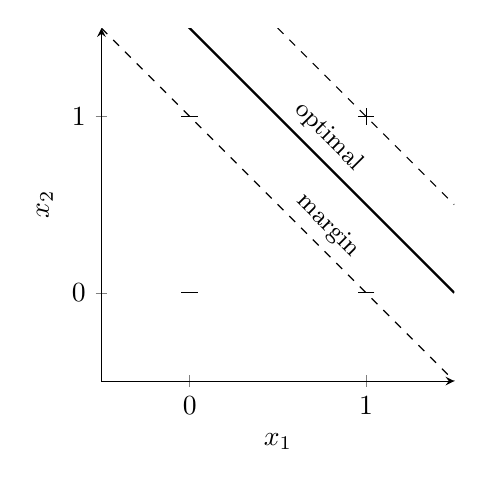
\begin{tikzpicture}
    \begin{axis}[
        axis x line=bottom,
        axis y line=left,
        xlabel={$x_1$},
        ylabel={$x_2$},
        width=0.5\textwidth,
        height=0.5\textwidth,
        xtick={0, 1},
        ytick={0, 1},
        xmin=-0.5, xmax=1.5,
        ymin=-0.5, ymax=1.5,
        domain=-0.5:1.5,
      ]
      \addplot+[only marks, mark=-, color=black, mark size=3pt] coordinates {
        (0, 0) (0, 1) (1, 0)
      };
      \addplot+[only marks, mark=+, color=black, mark size=3pt] coordinates {
        (1, 1)
      };
      \addplot+[mark=none, black, thick] {1.5 - x}
        node[above, pos=0.6, rotate=-45, font=\small] {optimal};
      \addplot+[mark=none, black, dashed] {1 - x}
        node[above, pos=0.6, rotate=-45, font=\small] {margin};
      \addplot+[mark=none, black, dashed] {2 - x};
    \end{axis}
  \end{tikzpicture}

  \small Support vectors: $(1, 0)$, $(0, 1)$, and $(1, 1)$.
\end{frame}

\begin{frame}{Maximal margin classifier --- properties}
  The classifier is built from \textbf{support vectors} only:
  \[
    f(x) = \sign\!\left(\sum_{i=1}^{n} y_i\, a_i\, (\vec{x}_i \cdot x) - b\right)
  \]
  where $a_i > 0$ for support vectors, $a_i = 0$ otherwise.

  \vspace{0.3cm}
  \begin{itemize}
    \item Number of parameters depends on data $\Rightarrow$ \textbf{nonparametric}
    \item Soft margin: allows $R_\text{emp} > 0$ for non-separable data
    \item Kernel trick: handle nonlinear problems
  \end{itemize}
\end{frame}

% ---- Takeaways ----

\begin{frame}{Takeaways}
  \begin{itemize}
    \item Optimal solutions establish how good a solution can possibly be
    \item Reducing error is not enough to guarantee a good solution
    \item Controlling model complexity is crucial for generalization
    \item The perceptron minimizes empirical risk (fixed complexity)
    \item The maximal margin classifier minimizes complexity (fixed risk)
  \end{itemize}
\end{frame}

% ---- End ----

\begin{frame}[standout]
  Questions?
\end{frame}

\end{document}

% slides/preprocessing.tex - Chapter 7: Data Preprocessing

% slides/preamble.tex - Shared preamble for all slide decks
% Metropolis theme with grayscale style matching the book

\documentclass[aspectratio=169]{beamer}

\usetheme{metropolis}

% ---------- Colors (grayscale) ----------
\definecolor{bookdark}{gray}{0.2}
\definecolor{bookgray}{gray}{0.5}
\definecolor{booklight}{gray}{0.92}

\setbeamercolor{normal text}{fg=bookdark, bg=white}
\setbeamercolor{alerted text}{fg=bookdark}
\setbeamercolor{frametitle}{fg=white, bg=bookdark}
\setbeamercolor{title separator}{fg=bookgray}
\setbeamercolor{progress bar}{fg=bookgray, bg=booklight}
\setbeamercolor{block title}{fg=white, bg=bookgray}
\setbeamercolor{block body}{fg=bookdark, bg=booklight}
\setbeamercolor{block title alerted}{fg=white, bg=bookdark}
\setbeamercolor{block body alerted}{fg=bookdark, bg=booklight}
\setbeamercolor{block title example}{fg=white, bg=bookgray}
\setbeamercolor{block body example}{fg=bookdark, bg=booklight}

\setbeamertemplate{frame numbering}[fraction]

% ---------- Fonts (matching the book) ----------
\usepackage[T1]{fontenc}
\usepackage{fontspec}
\usepackage[warnings-off={mathtools-colon,mathtools-overbracket}]{unicode-math}

\setmathfont{STIXTwoMath}[
  Extension={.otf},
  Path={./fonts/},
  Scale=1]

\setsansfont{STIXTwoText}[
  Extension={.otf},
  Path={./fonts/},
  UprightFont={*-Regular},
  BoldFont={*-Bold},
  ItalicFont={*-Italic},
  BoldItalicFont={*-BoldItalic}]

\setmainfont{STIXTwoText}[
  Extension={.otf},
  Path={./fonts/},
  UprightFont={*-Regular},
  BoldFont={*-Bold},
  ItalicFont={*-Italic},
  BoldItalicFont={*-BoldItalic}]

\setmonofont{CourierPrime}[
  Extension={.ttf},
  Path={./fonts/},
  UprightFont={*-Regular},
  BoldFont={*-Bold},
  ItalicFont={*-Italic},
  BoldItalicFont={*-BoldItalic},
  Scale=0.9]

% ---------- Packages ----------
\usepackage{amsmath}
\usepackage{mathtools}
\usepackage{graphicx}
\usepackage{booktabs}

% ---------- TikZ ----------
\usepackage{tikz}
\usetikzlibrary{shapes, arrows.meta, positioning, shapes.geometric, fit}

\tikzset{%
  decision/.style={draw, diamond, text centered, minimum height=0.5cm, minimum width=1cm},
  block/.style={rectangle, draw, text width=6em, text centered, rounded corners, minimum height=3em},
  mediumblock/.style={rectangle, draw, text width=3em, text centered, rounded corners, minimum height=2em},
  darkblock/.style={block, fill=gray, text=white},
  smallblock/.style={rectangle, rounded corners, draw, font=\tiny, minimum height=1em, inner sep=2pt},
  smalldarkblock/.style={smallblock, fill=gray, text=white},
  darkcircle/.style={draw, circle, fill=gray, text centered, text=white},
  smallcircle/.style={draw, circle, text centered, font=\tiny},
  smalldarkcircle/.style={smallcircle, fill=gray, text=white},
  line/.style={draw, -latex},
  dline/.style={draw, latex-latex},
  bigarrow/.style={draw, -latex, line width=3pt, gray},
}

% ---------- Math operators ----------
\DeclareMathOperator*{\argmax}{arg\,max}
\DeclareMathOperator*{\argmin}{arg\,min}
\DeclareMathOperator{\Prob}{P}
\DeclareMathOperator{\E}{E}
\DeclareMathOperator{\Var}{Var}
\DeclareMathOperator{\sign}{sign}
\DeclareMathOperator{\clamp}{clamp}

% ---------- Hyperref ----------
\usepackage{hyperref}
\hypersetup{colorlinks, urlcolor=bookgray, linkcolor=bookdark}

% ---------- Commands ----------
\renewcommand{\vec}[1]{\mathbf{#1}}
\newcommand{\code}[1]{\colorbox{black!10!white}{\texttt{#1}}}

% ---------- Book info, license, and disclaimer ----------
\newcommand{\bookframe}{%
  \begin{frame}{About these slides}
    These slides are companion material for the book

    \vspace{0.3cm}
    \begin{center}
      \textbf{Data Science Project: An Inductive Learning Approach}\\[2pt]
      Prof.~Dr.~Filipe A. N. Verri\\[4pt]
      \url{https://leanpub.com/dsp}
    \end{center}

    \vspace{0.3cm}
    All intellectual content comes from the book and is not AI-generated.
    Slides were produced with the assistance of
    \href{https://claude.ai/code}{Claude Code}.

    \vspace{0.3cm}
    {\small
    Licensed under
    \href{https://creativecommons.org/licenses/by-nc/4.0/}{CC BY-NC 4.0}.
    You are free to modify and redistribute this work as long as you give
    proper credit and do not use it for commercial purposes.}
  \end{frame}%
}

% ---------- TikZ color presets (used by book figures) ----------
\colorlet{circle edge}{black!50}
\colorlet{circle area}{black!20}
\tikzset{
  filled/.style={fill=circle area, draw=circle edge, thick},
  outline/.style={draw=circle edge, thick},
}


\title{Data Preprocessing}
\subtitle{Data Science Project: An Inductive Learning Approach}
\author{Prof.~Dr.~Filipe A. N. Verri}
\date{}

\begin{document}

\maketitle
\bookframe

% ---- Epigraph ----

\begin{frame}{}
  \vfill
  \begin{quote}
    I find your lack of faith disturbing.
    \begin{flushright}
      --- Darth Vader, \textit{Star Wars: Episode IV} (1977)
    \end{flushright}
  \end{quote}
  \vfill
\end{frame}

% ---- Overview ----

\begin{frame}{Overview}
  \begin{columns}[T]
    \begin{column}{0.48\textwidth}
      \textbf{Contents}
      \begin{itemize}
        \item Introduction
        \item Data cleaning
        \item Data sampling
        \item Data transformation
      \end{itemize}
    \end{column}
    \begin{column}{0.48\textwidth}
      \textbf{Objectives}
      \begin{itemize}
        \item Understand the main data preprocessing tasks and techniques
        \item Learn the behavior of the preprocessing chain (fitting, adjustment,
          application)
      \end{itemize}
    \end{column}
  \end{columns}
\end{frame}

% ===========================================================================
\section{Introduction}
% ===========================================================================

\begin{frame}{Why preprocess?}
  \begin{itemize}
    \item Tidy data is not necessarily suitable for modeling
    \item Example: perceptron requires \textbf{numerical} inputs
    \item Preprocessing adjusts data for the chosen learning machine
    \item Operations are \textbf{dependent on the learning method}
  \end{itemize}
\end{frame}

\begin{frame}{Three steps of a preprocessing technique}
  \begin{enumerate}
    \item \textbf{Fitting}: parameters adjusted to the training data
    \item \textbf{Adjustment}: training data transformed according to
      fitted parameters (may change sample size/distribution)
    \item \textbf{Applying}: operation applied to new data, sample by sample
  \end{enumerate}

  \vspace{0.3cm}
  Understanding these steps is crucial to avoid \textbf{data leakage}.
\end{frame}

\begin{frame}{Formal definition}
  Strategy $F$ takes a table $T = (K, H, c)$ and returns:
  \begin{itemize}
    \item Adjusted table $T' = (K', H', c')$
    \item Fitted preprocessor $f_\phi(z)$
  \end{itemize}

  \vspace{0.3cm}
  A chain of operations $F_1, \ldots, F_m$:
  \[
    f(z; \phi) = \left(f_{\phi_1} \circ \cdots \circ f_{\phi_m}\right)(z)
  \]
  Each operation depends on the result of the previous ones.
\end{frame}

\begin{frame}{Degeneration}
  The preprocessor \textbf{degenerates} over tuple $z$ if $f_\phi(z) = (?, \ldots, ?)$.

  \vspace{0.3cm}
  \begin{itemize}
    \item Unexpected values, incomplete information, \ldots
    \item If any step $f_{\phi_i}$ degenerates, the whole chain degenerates
    \item Developer must define a \textbf{default behavior}:
      \begin{itemize}
        \item Return a default value
        \item Redirect to a different model
        \item Raise an error/warning
      \end{itemize}
  \end{itemize}
\end{frame}

\begin{frame}{Preprocessing task categories}
  \begin{enumerate}
    \item \textbf{Data cleaning} --- remove errors and inconsistencies
    \item \textbf{Data sampling} --- select or create variations of the training set
    \item \textbf{Data transformation} --- adjust types and variables for modeling
  \end{enumerate}

  \vspace{0.3cm}
  Presented in typical application order (not fixed).
\end{frame}

% ===========================================================================
\section{Data cleaning}
% ===========================================================================

% ---------------------------------------------------------------------------
\subsection{Treating inconsistent data}
% ---------------------------------------------------------------------------

\begin{frame}{Treating inconsistent data}
  Three common tasks (parameters \textbf{not fitted} from data):
  \begin{itemize}
    \item \textbf{Unit conversion} --- ensure same units across columns
    \item \textbf{Range check} --- validate values within expected bounds
    \item \textbf{Category standardization} --- unify different representations
  \end{itemize}

  \vspace{0.3cm}
  Could be done in data handling, but having them in the preprocessor
  ensures consistent treatment of new data in production.
\end{frame}

\begin{frame}{Unit conversion}
  \centering\small
  \rowcolors{2}{black!10!white}{}
  \begin{tabular}{lp{8cm}}
    \toprule
    \multicolumn{2}{c}{\textbf{Unit conversion}} \\
    \midrule
    \textbf{Goal} &
      Convert physical quantities into the same unit of measurement. \\
    \textbf{Fitting} &
      None. User declares units and conversion factors. \\
    \textbf{Adjustment} &
      Sample by sample, independently. \\
    \textbf{Applying} &
      Converts values and drops the unit column. \\
    \bottomrule
  \end{tabular}
\end{frame}

\begin{frame}{Range check}
  \centering\small
  \rowcolors{2}{black!10!white}{}
  \begin{tabular}{lp{8cm}}
    \toprule
    \multicolumn{2}{c}{\textbf{Range check}} \\
    \midrule
    \textbf{Goal} &
      Check whether values are within the expected range. \\
    \textbf{Fitting} &
      None. User declares the valid range $[a, b]$. \\
    \textbf{Adjustment} &
      Sample by sample; degenerated samples may be removed. \\
    \textbf{Applying} &
      If $x \notin [a, b]$: replace with $?$, clamp to $[a, b]$, or degenerate. \\
    \bottomrule
  \end{tabular}
\end{frame}

\begin{frame}{Category standardization}
  \centering\small
  \rowcolors{2}{black!10!white}{}
  \begin{tabular}{lp{8cm}}
    \toprule
    \multicolumn{2}{c}{\textbf{Category standardization}} \\
    \midrule
    \textbf{Goal} &
      Map different names to a single canonical form. \\
    \textbf{Fitting} &
      None. User declares the mapping. \\
    \textbf{Adjustment} &
      Sample by sample, independently. \\
    \textbf{Applying} &
      Case standardization, special character removal, dictionary/fuzzy matching. \\
    \bottomrule
  \end{tabular}
\end{frame}

% ---------------------------------------------------------------------------
\subsection{Outlier detection}
% ---------------------------------------------------------------------------

\begin{frame}{Outlier detection}
  \begin{itemize}
    \item Observations significantly different from the rest
    \item Caused by errors or mixed phenomena
    \item Standard approach: remove outliers from the dataset
    \item Per-variable: replace outlier values with missing data
  \end{itemize}

  \vspace{0.3cm}
  \textbf{IQR heuristic:} Given $Q_1$, $Q_3$, and $\text{IQR} = Q_3 - Q_1$,\\
  a value is an outlier if $x < Q_1 - 1.5\,\text{IQR}$ or
  $x > Q_3 + 1.5\,\text{IQR}$.
\end{frame}

\begin{frame}{Outlier detection --- IQR}
  \centering\small
  \rowcolors{2}{black!10!white}{}
  \begin{tabular}{lp{8cm}}
    \toprule
    \multicolumn{2}{c}{\textbf{Outlier detection using the IQR}} \\
    \midrule
    \textbf{Goal} &
      Detect outliers using the IQR. \\
    \textbf{Fitting} &
      Store $Q_1$ and $Q_3$ for each variable. \\
    \textbf{Adjustment} &
      Sample by sample, independently. \\
    \textbf{Applying} &
      Replaces outlier values with missing data. \\
    \bottomrule
  \end{tabular}

  \vspace{0.5cm}
  \raggedright\small
  More advanced: One-Class SVM\footfullcite{Scholkopf2001} for generalizable outlier classification.
\end{frame}

\begin{frame}{Outlier removal}
  \centering\small
  \rowcolors{2}{black!10!white}{}
  \begin{tabular}{lp{8cm}}
    \toprule
    \multicolumn{2}{c}{\textbf{Outlier removal}} \\
    \midrule
    \textbf{Goal} &
      Remove observations that are outliers. \\
    \textbf{Fitting} &
      Parameters of the outlier classifier. \\
    \textbf{Adjustment} &
      Sample by sample; degenerated samples removed. \\
    \textbf{Applying} &
      Degenerates if classified as outlier; pass-through otherwise. \\
    \bottomrule
  \end{tabular}

  \vspace{0.3cm}
  \raggedright\small
  Developer must specify default behavior when an outlier is detected in production.
\end{frame}

% ---------------------------------------------------------------------------
\subsection{Treating missing data}
% ---------------------------------------------------------------------------

\begin{frame}{Treating missing data}
  Most models cannot handle missing data. Four strategies:
  \begin{enumerate}
    \item Remove \textbf{rows} with missing data
    \item Remove \textbf{columns} with missing data
    \item \textbf{Impute} the missing values
    \item \textbf{Indicator variable} + imputation
  \end{enumerate}

  \vspace{0.3cm}
  Removing rows ``on demand'' can change the data distribution,
  especially if data is not missing at random.
\end{frame}

\begin{frame}{Row removal (missing data)}
  \centering\small
  \rowcolors{2}{black!10!white}{}
  \begin{tabular}{lp{8cm}}
    \toprule
    \multicolumn{2}{c}{\textbf{Row removal based on missing data}} \\
    \midrule
    \textbf{Goal} &
      Remove observations with missing data in specified variables. \\
    \textbf{Fitting} &
      None. Variables to check are declared beforehand. \\
    \textbf{Adjustment} &
      Sample by sample; degenerated samples removed. \\
    \textbf{Applying} &
      Degenerates over rows with missing data in specified variables. \\
    \bottomrule
  \end{tabular}
\end{frame}

\begin{frame}{Column removal (missing data)}
  \centering\small
  \rowcolors{2}{black!10!white}{}
  \begin{tabular}{lp{8cm}}
    \toprule
    \multicolumn{2}{c}{\textbf{Column removal based on missing data}} \\
    \midrule
    \textbf{Goal} &
      Remove variables with missing data. \\
    \textbf{Fitting} &
      Mark all variables with missing data in the training set. \\
    \textbf{Adjustment} &
      Marked columns are dropped. \\
    \textbf{Applying} &
      Drops the same columns chosen during fitting. \\
    \bottomrule
  \end{tabular}

  \vspace{0.3cm}
  \raggedright\small
  Valuable information may be lost when removing columns for all samples.
\end{frame}

\begin{frame}{Imputation}
  \centering\small
  \rowcolors{2}{black!10!white}{}
  \begin{tabular}{lp{8cm}}
    \toprule
    \multicolumn{2}{c}{\textbf{Imputation of missing data}} \\
    \midrule
    \textbf{Goal} &
      Replace missing data with a statistic (mean, median, mode). \\
    \textbf{Fitting} &
      Statistic computed from available training data. \\
    \textbf{Adjustment} &
      Sample by sample, independently. \\
    \textbf{Applying} &
      Replaces missing values; optionally creates an indicator variable. \\
    \bottomrule
  \end{tabular}

  \vspace{0.3cm}
  \raggedright\small
  Indicator variable: useful when missingness itself is informative\\
  (e.g., ``days since last pregnancy'' is missing if male or zero children).
\end{frame}

% ===========================================================================
\section{Data sampling}
% ===========================================================================

\begin{frame}{Data sampling}
  After cleaning, select or create variations of the training set:
  \begin{itemize}
    \item \textbf{Random sampling} --- reduce dataset size
    \item \textbf{Scope filtering} --- reduce the modeled phenomenon's scope
    \item \textbf{Class balancing} --- equalize class representation
  \end{itemize}
\end{frame}

% ---------------------------------------------------------------------------
\subsection{Random sampling}
% ---------------------------------------------------------------------------

\begin{frame}{Random sampling}
  \centering\small
  \rowcolors{2}{black!10!white}{}
  \begin{tabular}{lp{8cm}}
    \toprule
    \multicolumn{2}{c}{\textbf{Random sampling}} \\
    \midrule
    \textbf{Goal} &
      Select a random subset of the training data. \\
    \textbf{Fitting} &
      None. User declares the sample size. \\
    \textbf{Adjustment} &
      Rows randomly chosen. \\
    \textbf{Applying} &
      \textbf{Pass-through}: does nothing with new data. \\
    \bottomrule
  \end{tabular}
\end{frame}

% ---------------------------------------------------------------------------
\subsection{Scope filtering}
% ---------------------------------------------------------------------------

\begin{frame}{Scope filtering}
  \centering\small
  \rowcolors{2}{black!10!white}{}
  \begin{tabular}{lp{8cm}}
    \toprule
    \multicolumn{2}{c}{\textbf{Scope filtering}} \\
    \midrule
    \textbf{Goal} &
      Remove observations that do not satisfy a predefined rule. \\
    \textbf{Fitting} &
      None. User declares the rule. \\
    \textbf{Adjustment} &
      Sample by sample; degenerated samples removed. \\
    \textbf{Applying} &
      Degenerates over samples that violate the rule. \\
    \bottomrule
  \end{tabular}

  \vspace{0.3cm}
  \raggedright\small
  Variation: \textbf{model trees} --- shallow decision trees that branch into
  different models at each leaf.
\end{frame}

% ---------------------------------------------------------------------------
\subsection{Class balancing}
% ---------------------------------------------------------------------------

\begin{frame}{Class balancing}
  \centering\small
  \rowcolors{2}{black!10!white}{}
  \begin{tabular}{lp{8cm}}
    \toprule
    \multicolumn{2}{c}{\textbf{Class balancing}} \\
    \midrule
    \textbf{Goal} &
      Balance the number of observations in each class. \\
    \textbf{Fitting} &
      User declares or calculates target class sizes. \\
    \textbf{Adjustment} &
      Undersample (random removal) or oversample (resampling). \\
    \textbf{Applying} &
      \textbf{Pass-through}: does nothing with new data. \\
    \bottomrule
  \end{tabular}

  \vspace{0.3cm}
  \raggedright\small
  Advanced: SMOTE\footfullcite{chawla2002smote} creates synthetic minority samples without repetition.
\end{frame}

% ===========================================================================
\section{Data transformation}
% ===========================================================================

\begin{frame}{Data transformation}
  Data is now clean and well-sampled. Transform columns to suit the model:
  \begin{itemize}
    \item \textbf{Type conversion} --- categorical $\leftrightarrow$ numerical
    \item \textbf{Normalization} --- scale values to expected ranges
    \item \textbf{Dimensionality reduction} --- reduce number of variables
    \item \textbf{Data enhancement} --- add external information
  \end{itemize}
\end{frame}

% ---------------------------------------------------------------------------
\subsection{Type conversion}
% ---------------------------------------------------------------------------

\begin{frame}{Categorical to numerical}
  \textbf{Label encoding:}
  \begin{itemize}
    \item Replace $x \in \{a, b, c\}$ with $x' \in \{1, 2, 3\}$
    \item Suitable when there is a natural order $a < b < c$
  \end{itemize}

  \vspace{0.3cm}
  \textbf{One-hot encoding:}
  \begin{itemize}
    \item Create a new column for each category
    \item Column $= 1$ if present, $0$ otherwise
    \item Group rare categories into an \emph{other} column
  \end{itemize}
\end{frame}

\begin{frame}{One-hot encoding}
  \centering\small
  \rowcolors{2}{black!10!white}{}
  \begin{tabular}{lp{8cm}}
    \toprule
    \multicolumn{2}{c}{\textbf{One-hot encoding}} \\
    \midrule
    \textbf{Goal} &
      Create a new column for each category value. \\
    \textbf{Fitting} &
      Store the unique values; optionally mark an \emph{other} category. \\
    \textbf{Adjustment} &
      Sample by sample, independently. \\
    \textbf{Applying} &
      New columns filled with $1$ or $0$; unknown values assigned to \emph{other}. \\
    \bottomrule
  \end{tabular}
\end{frame}

\begin{frame}{Numerical to categorical (binning)}
  \centering\small
  \rowcolors{2}{black!10!white}{}
  \begin{tabular}{lp{8cm}}
    \toprule
    \multicolumn{2}{c}{\textbf{Binning numerical values}} \\
    \midrule
    \textbf{Goal} &
      Create a categorical column from a numerical one. \\
    \textbf{Fitting} &
      Store the range of each bin (by frequency or by range). \\
    \textbf{Adjustment} &
      Sample by sample, independently. \\
    \textbf{Applying} &
      Assigns each value to the corresponding bin. \\
    \bottomrule
  \end{tabular}

  \vspace{0.3cm}
  \raggedright\small
  Also common: converting dates/intervals to numerical differences
  (e.g., birth date $\to$ age).
\end{frame}

% ---------------------------------------------------------------------------
\subsection{Normalization}
% ---------------------------------------------------------------------------

\begin{frame}{Standardization}
  \[
    x' = \frac{x - \mu}{\sigma}
  \]

  \centering\small
  \rowcolors{2}{black!10!white}{}
  \begin{tabular}{lp{8cm}}
    \toprule
    \multicolumn{2}{c}{\textbf{Standardization}} \\
    \midrule
    \textbf{Goal} &
      Scale values in a column (zero mean, unit variance). \\
    \textbf{Fitting} &
      Store $\mu$ and $\sigma$ from the training set. \\
    \textbf{Adjustment} &
      Sample by sample, independently. \\
    \textbf{Applying} &
      Scales values using the fitted $\mu$ and $\sigma$. \\
    \bottomrule
  \end{tabular}
\end{frame}

\begin{frame}{Rescaling}
  \[
    x' = a + (b - a) \, \frac{x - x_\text{min}}{x_\text{max} - x_\text{min}}
  \]

  \centering\small
  \rowcolors{2}{black!10!white}{}
  \begin{tabular}{lp{8cm}}
    \toprule
    \multicolumn{2}{c}{\textbf{Rescaling}} \\
    \midrule
    \textbf{Goal} &
      Rescale values to a target range $[a, b]$. \\
    \textbf{Fitting} &
      Store $x_\text{min}$ and $x_\text{max}$ from the training set. \\
    \textbf{Adjustment} &
      Sample by sample, independently. \\
    \textbf{Applying} &
      Rescales and clamps: $\max(a, \min(b, x'))$. \\
    \bottomrule
  \end{tabular}
\end{frame}

% ---------------------------------------------------------------------------
\subsection{Dimensionality reduction}
% ---------------------------------------------------------------------------

\begin{frame}{Dimensionality reduction}
  \textbf{Feature selection:}
  \begin{itemize}
    \item Select a subset of existing variables
    \item Example: rank by mutual information with target, keep top $k$
  \end{itemize}

  \vspace{0.3cm}
  \textbf{Feature extraction:}
  \begin{itemize}
    \item Create new variables as combinations of original ones
    \item Linear: PCA
    \item Non-linear: autoencoders
    \item Drawback: new variables are hard to interpret
  \end{itemize}
\end{frame}

% ---------------------------------------------------------------------------
\subsection{Data enhancement}
% ---------------------------------------------------------------------------

\begin{frame}{Data enhancement}
  \centering\small
  \rowcolors{2}{black!10!white}{}
  \begin{tabular}{lp{8cm}}
    \toprule
    \multicolumn{2}{c}{\textbf{Data enhancement}} \\
    \midrule
    \textbf{Goal} &
      Enrich the dataset with external information. \\
    \textbf{Fitting} &
      Store the external dataset and the join column. \\
    \textbf{Adjustment} &
      Left join with external dataset (same number of rows). \\
    \textbf{Applying} &
      Enhances each new observation with external information. \\
    \bottomrule
  \end{tabular}

  \vspace{0.3cm}
  \raggedright\small
  Example: join zip codes with socioeconomic data.
\end{frame}

% ---------------------------------------------------------------------------
\subsection{Unstructured data}
% ---------------------------------------------------------------------------

\begin{frame}{Comments on unstructured data}
  \begin{itemize}
    \item Any unstructured data can be transformed into structured data
    \item Bag of words, word embeddings, signal/image processing
    \item Modern methods (CNNs) learn preprocessing and model jointly
      \begin{itemize}
        \item Convolutional layers $=$ learned feature extraction
      \end{itemize}
    \item Unstructured data is a vast field, out of scope of this book
  \end{itemize}
\end{frame}

% ---- Takeaways ----

\begin{frame}{Takeaways}
  \begin{itemize}
    \item Each learning method requires specific preprocessing tasks
    \item Fitting the preprocessor is crucial to avoid leakage
    \item Default behavior when the chain degenerates must be specified
    \item Three categories: cleaning, sampling, transformation
    \item Preprocessing parameters are fitted, not fixed
  \end{itemize}
\end{frame}

% ---- End ----

\begin{frame}[standout]
  Questions?
\end{frame}

\end{document}

\chapter{Solution validation}
\label{chap:planning}
\glsresetall

\chapterprecishere{%
  All models are wrong, but some are useful.
  \par\raggedleft--- \textup{George E. P. Box}, Robustness in Statistics}

Once we have defined what an inductive problem is and the means to solve it, we need to
think about how to validate the solution.

In this chapter, we present the experimental planning that one can use in the data-driven
parts of a data science project.  \emph{Experimental planning}  in the context of data
science involves designing and organizing experiments to gather performance data
systematically in order to reach specific goals or test hypotheses.

The reason we need to plan experiments is that data science is experimental, i.e., we
usually lack a theoretical model that can predict the outcome of a given algorithm on a
given dataset.  This is why we need to run experiments to gather performance data and make
inferences from it.  The stochastic nature of data and of the learning process makes it
more difficult to predict the outcome of a given algorithm on a given dataset.  Robust
experimental planning is essential to ensure that the results of the experiments are
reliable and can be used to make decisions.

Moreover, we need to understand the main metrics that are used to evaluate the performance
of a solution --- i.e., the pair preprocessor and model.  Each learning task has different
metrics, and the goals of the project will determine which metrics are more important.

There is not a single way to plan experiments, but there are some common steps that can
be followed to design a good experimental plan.  In this chapter, we present a
framework for experimental planning that can be used in most data science projects
for inductive problems.

\begin{mainbox}{Chapter remarks}

  \boxsubtitle{Contents}

  \startcontents[chapters]
  \printcontents[chapters]{}{1}{}
  \vspace{1em}

  \boxsubtitle{Context}

  \begin{itemize}
    \itemsep0em
    \item Before putting a solution into production, we need to validate it.
    \item The validation process is experimental.
  \end{itemize}

  \boxsubtitle{Objectives}

  \begin{itemize}
    \itemsep0em
    \item Understand the importance of experimental planning.
    \item Learn the main evaluation metrics used in predictive tasks.
    \item Learn how to design an experimental plan to validate a solution.
  \end{itemize}

  \boxsubtitle{Takeaways}

  \begin{itemize}
    \itemsep0em
    \item Evaluation metrics should be chosen according to the goals of the project.
    \item The experimental plan should be designed to gather performance data
      systematically.
    \item A hypothesis test can be used to validate the results of the experiments.
  \end{itemize}
\end{mainbox}

{}
\clearpage

\section{Evaluation}
\label{sec:evaluation}

One fundamental step in the validation of a data-driven solution for a task is the
\emph{evaluation} of the pair preprocessor and model. This chapter presents strategies to
measure performance of
classifiers and regressors, and how to interpret the results.

We consider the following setup.  Let $T = (K, H, c)$ be a table that represents the data
in the desired observational unit --- as defined in \cref{sec:formal-structured-data}.
Without loss of generality --- as the keys are not used in the modeling process ---, we
can consider $K = \{1, 2, \dots\}$ such that $\rowcard[i] = 1$, if $i \in \{1, \dots,
n\}$, and $\rowcard[i] = 0$, otherwise.  That means that every row $r \in \{1, \dots, n\}$
is present in the table.

The table is split into two sets: a training set, given by indices (or keys)
$\mathcal{I}_\text{training} \in \{1, \dots, n\}$, and a test set, given by indices
$\mathcal{I}_\text{test} \in \{1, \dots, n\}$, such that $$\mathcal{I}_\text{training}
\cap \mathcal{I}_\text{test} = \emptyset$$ and $$\mathcal{I}_\text{training} \cup
\mathcal{I}_\text{test} = \{1,\dots,n\}\text{.}$$

The bridge between the table format (\cref{def:itable}) and the data format used in the
learning process (as described in \cref{sec:learning-problem}) is explained in the
following.  We say that the pair $(\vec{x}_i, y_i)$ contains the feature vector $\vec{x}_i$
and the target value $y_i$ of the sample with key $i$ in table $T$.  Mathematically,
given target variable $h \in H$, we have that $y_i = c(i, h)$ and $\vec{x}_i$ is the tuple
$$\big(c(i, h') : h' \in H \setminus \left\{ h \right\}\big)\text{.}$$

For evaluation, we consider a data preprocessing technique $F$ and a learning machine
$M$.  The following steps are taken.

\paragraph{Preprocessing}

Preprocessing technique $F$ is applied to the training set $T_\text{training} = (K, H,
c_\text{training})$ where \[
  c_\text{training}(i, h) = \begin{cases}
    c(i, h) & \text{if } i \in \mathcal{I}_\text{training}\text{,} \\
    () & \text{otherwise}\text{.}
  \end{cases}
\]  The result is an adjusted training set $T'_\text{training}$ and a fitted
preprocessor $f(\vec{x}; \phi) \equiv f_\phi(\vec{x})$, where $\vec{x} \in \mathcal{X}$
for some space $\mathcal{X}$ that does not include (or does not modify) the target
variable --- consult \cref{sub:formal-preprocessing}.  Note that, by definition, the size
of the adjusted training set can be different from the original due to sampling or
filtering.  The hard requirement is that the target variable $h$ is not changed.

\paragraph{Learning}

The learning machine $M$ is trained on the adjusted training set $D'_\text{training} =
\{(\vec{x}'_i, y'_i)\}$, where pairs $(\vec{x}'_i, y'_i)$ come from the table
$T'_\text{training}$.  The result is a model $f(\vec{x}'; \theta) \equiv
f_\theta(\vec{x}')$ --- consult \cref{chap:slt}.

\paragraph{Transformation}

The preprocessor $f_\phi$ is applied to the test set $T_\text{test} = (K, H,
c_\text{test})$ where \[
  c_\text{test}(i, h) = \begin{cases}
    c(i, h) & \text{if } i \in \mathcal{I}_\text{test}\text{,} \\
    () & \text{otherwise}\text{.}
  \end{cases}
\]  The result is a preprocessed test set $T'_\text{test}$ from which we can obtain the
set $D'_\text{test} = \{(\vec{x}'_i, y_i) : i \in \mathcal{I}_\text{test}\}$ such
that $\vec{x}'_i = f_\phi(\vec{x}_i)$.  Note that, to avoid \gls{leakage} and other
issues, the preprocessor has no access to the target values $y_i$ (even if the
adjusted training set uses the label somehow).

\paragraph{Prediction}

The model $f_\theta$ is used to make predictions on the preprocessed test set
$D'_\text{test}$ to obtain predicted values $\hat{y}_i = f_\theta(\vec{x}'_i)$ for all
$i \in \mathcal{I}_\text{test}$.

\paragraph{Evaluation}

By comparing $\hat{y}_i$ with $y_i$ for all $i \in \mathcal{I}_\text{test}$, we
evaluate how well the choice of $\phi$ (parameters of the preprocessor) and $\theta$
(parameters of the model) is.

\subsection{Binary classification evaluation}

To assess the quality of a solution for a binary classification task, we need to know which
samples in the test set were classified into which classes.  This information is
summarized in the \emph{confusion matrix}, which is the basis for performance metrics in
classification tasks.

\subsubsection{Confusion matrix}

The confusion matrix is a table where the rows represent the true classes and the columns
represent the predicted classes.  The diagonal of the matrix represents the correct
classifications, while the off-diagonal elements represent errors.  For binary
classification, the confusion matrix is given by
\begin{equation*}
  \begin{blockarray}{cccc}
    & & \multicolumn{2}{c}{\text{Predicted}} \\
    & & 1 & 0 \\
    \begin{block}{l c (c c)}
      \text{Expected} & 1 & \text{TP} & \text{FN} \\
      & 0 & \text{FP} & \text{TN} \\
    \end{block}
  \end{blockarray}
\end{equation*}
where TP is the number of true positives
$$|\{ i \in \mathcal{I}_\text{test} : y_i = 1 \land \hat{y}_i = 1 \}|\text{,}$$
TN is the number of true negatives
$$|\{ i \in \mathcal{I}_\text{test} : y_i = 0 \land \hat{y}_i = 0 \}|\text{,}$$
FN is the number of false negatives
$$|\{ i \in \mathcal{I}_\text{test} : y_i = 1 \land \hat{y}_i = 0 \}|\text{,}$$
and FP is the number of false positives
$$|\{ i \in \mathcal{I}_\text{test} : y_i = 0 \land \hat{y}_i = 1 \}|\text{.}$$

\subsubsection{Performance metrics}

From the confusion matrix, we can derive several performance metrics.  Each of them focuses
on different aspects of the classification task, and the choice of the metric depends on
the problem at hand.  Each metric prioritizes different types of errors and yields
a value between 0 and 1, where 1 is the best possible value.

\paragraph{Accuracy} is the proportion of correct predictions over the total number of
samples in the test set, given by
\begin{equation*}
  \text{Accuracy} = \frac{\text{TP} + \text{TN}}{\text{TP} + \text{TN} + \text{FP} + \text{FN}}\text{.}
\end{equation*}
This metric is simple and easy to interpret: a classifier with an accuracy of 1 is
perfect, while a classifier with an accuracy of 0.5 misses half of the predictions.
Accuracy assigns the same weight to any kind of error --- i.e., false positives and false
negatives.  As a result, if the proportion of positive and negative samples is imbalanced,
the value of accuracy may become misleading.  Let $\pi$ be the ratio of positive samples in
the test set --- consequently, $1-\pi$ is the ratio of negative samples ---, then a
classifier that correctly predicts all positive samples and none of the negative samples
will have an accuracy of $\pi$.  If $\pi$ is close to 1, the classifier will have a high value
of accuracy even if it is not good at predicting the negative class.

This issue is not impeditive for the usage of accuracy in imbalanced datasets, but one
needs to be aware that accuracy values lower than $\max(\pi, 1-\pi)$ are not better than
guessing.

\paragraph{Balanced accuracy} aims to solve this interpretation issue of the accuracy.  It
is the average of the true positive rate (TPR) and the true negative rate (TNR), given by
\begin{equation*}
  \text{Balanced Accuracy} = \frac{\text{TPR} + \text{TNR}}{2}\text{,}
\end{equation*}
where
\[
  \text{TPR} = \frac{\text{TP}}{\text{TP} + \text{FN}}\text{,}
\]
and
\[
  \text{TNR} = \frac{\text{TN}}{\text{TN} + \text{FP}}\text{.}
\]
Each term penalizes a different type of error independently: TPR penalizes false
negatives, while TNR penalizes false positives.  Balanced accuracy is useful when the cost
of errors on the minority class is higher than the cost of errors on the majority class.
This way, any value greater than 0.5 is better than random guessing.

A limitation of the balanced accuracy is that it ``automatically'' assigns the weight of
errors based on the class proportion, which may not be the best choice for the problem.
Other metrics focus only on one of the classes and are more flexible to adjust the weight of
errors.

\paragraph{Precision} is an asymmetrical metric that focuses on the positive class.  It is
the proportion of true positive predictions over the total number of samples predicted as
positive, given by
\begin{equation*}
  \text{Precision} = \frac{\text{TP}}{\text{TP} + \text{FP}}\text{.}
\end{equation*}
This metric is useful when the cost of false alarms is high, as it quantifies the
ability of the classifier to avoid false positives.  For example, in a medical diagnosis
task, precision is important to avoid unnecessary treatments (false positive diagnoses).
Semantically, precision measures how confident we can be that a positive prediction is
actually positive.  Note that it measures nothing about the ability of the classifier in
terms of the negative predictions.

\paragraph{Recall} is another asymmetrical metric that also focuses on the positive class.
It is the proportion of true positive predictions over the total number of
samples that are actually positive, given by
\begin{equation*}
  \text{Recall} = \text{TPR} = \frac{\text{TP}}{\text{TP} + \text{FN}}\text{.}
\end{equation*}
This metric is useful when the cost of missing a positive sample is high, as it quantifies the
ability of the classifier to avoid false negatives.  It can also be interpreted as the
``completeness'' of the classifier: how many positive samples were correctly retrieved.
For example, in a medical diagnosis task, recall is important to avoid missing a
diagnosis.

\paragraph{F-score} is a way of balancing both kinds of errors, false positives and false
negatives, while maintaining the focus on the positive class. It is the weighted harmonic
mean of precision and recall given by
\begin{equation*}
  \text{F-score}(\beta) = \text{F}_\beta\text{-score} =
    \frac%
      {(1 + \beta^2) \cdot \text{Precision} \cdot \text{Recall}}
      {\beta^2 \cdot \text{Precision} + \text{Recall}}\text{,}
\end{equation*}
where $\beta > 0$ is a parameter that controls the weight of precision in the metric.
The most common value for $\beta$ is 1, which gives the F$_1$-score.  Higher values of
$\beta$ give more weight to precision ($\beta > 1$), while lower values give more weight
to recall ($0 < \beta < 1$).

\paragraph{Specificity} goes in the opposite direction of recall, focusing on the negative
class.  It is the proportion of true negative predictions over the total
number of samples that are actually negative, given by
\begin{equation*}
  \text{Specificity} = \text{TNR} = \frac{\text{TN}}{\text{TN} + \text{FP}}\text{.}
\end{equation*}
This metric is very common in the medical literature, but less common in other contexts.
The probable reason is that it is easier to interpret the metrics that focus on the
positive class, as the negative class is usually the majority class --- and, thus, less
interesting.

\subsubsection{Interpretation of metrics}

\Cref{tab:classification-metrics} summarizes the properties of the classification
performance metrics.  Accuracy and balanced accuracy are good metrics when no particular
class is more important than the other.  Remember, however, that balanced accuracy gives
more weight to errors on the minority class.  Precision and recall are useful to evaluate
the performance of the solution in terms of the positive class.  They are complementary metrics,
and looking at only one of them may give a biased view of the performance --- more on that
below.  The F-score is a way to balance precision and recall with a controllable parameter.

\begin{tablebox}[label=tab:classification-metrics]{Summary of the properties of
  data classification performance metrics.}
  \centering
  \rowcolors{2}{black!10!white}{}
  \begin{tabular}{l c c}
    \toprule
    \textbf{Metric} & \textbf{Focus} & \textbf{Interpretation} \\
    \midrule
    Accuracy           & Symmetrical & Penalizes all \\
    Balanced Accuracy  & Symmetrical & Penalizes all (weighted) \\
    Recall (TPR)       & Positive & Penalizes FN \\
    Precision          & Positive & Penalizes FP \\
    F-score            & Positive & Penalizes all (weighted) \\
    Specificity (TNR)  & Negative & Penalizes FP \\
    % Fall-out (FPR)     & Negative & Not affected & Penalizes TN \\
    % FPR = 1 - TNR
    \bottomrule
  \end{tabular}
\end{tablebox}

A common misconception about the asymmetrical metrics (especially precision) is that they
are always robust to class imbalance.  Observe \cref{tab:classification-metrics-ex}, which shows
the behavior of the classification performance metrics for three (useless) classifiers: one
that always predicts the positive class (Guess 1), another that always predicts the
negative class (Guess 0), and a classifier that randomly guesses the class independently
of the class priors (Random).

\begin{tablebox}[label=tab:classification-metrics-ex]{Behavior of classification
  performance metrics for different classifiers.}
  \centering
  \rowcolors{2}{black!10!white}{}
  \begin{tabular}{l c c c}
    \toprule
    \textbf{Metric} & \textbf{Guess 1} & \textbf{Guess 0} & \textbf{Random} \\
    \midrule
    Accuracy$^\dagger$ & $\pi$ & $1 - \pi$ & $0.5$ \\
    Balanced Accuracy & $0.5$ & $0.5$ & $0.5$ \\
    Recall (TPR) & $1$ & $0$ & $0.5$ \\
    Precision$^\dagger$ & $\pi$ & $0/0 = 0$ & $\pi$ \\
    F$_1$-score$^\dagger$ & $\frac{2 \pi}{1 + \pi}$ & 0 & $\frac{2 \pi}{1 + 2\pi}$ \\
    Specificity (TNR) & $0$ & $1$ & $0.5$ \\
    \bottomrule
  \end{tabular}
  \tcblower
  Performance of different classifiers in the example of a dataset with ratio $\pi$ of
  positive and $1-\pi$ of negative samples.  Metrics affected by class imbalance are
  marked with $^\dagger$.
\end{tablebox}

We can see that, as $\pi \to 1$, i.e. the positive class dominates the dataset, guessing
the positive class achieves maximum values for metrics like accuracy, precision, and
F$_1$-score.  Even for random guessing the class, precision (and F$_1$-score) is affected
by the class imbalance, yielding $1$ (and $2/3$) as $\pi \to 1$.  As a result, these
metrics should be preferred when the positive class is the minority class, so the results
are not erroneously inflated --- and, consequently, mistakenly interpreted as good.
\textcite{Williams2021}\footfullcite{Williams2021} provides an interesting discussion on
that.

Finally, besides accuracy, the other metrics do not behave well when the evaluation set is
too small.  In this case, the metrics may be too sensitive to the particular samples in
the test set or may not be able to be calculated at all.

\subsection{Regression estimation evaluation}

Performance metrics for regression tasks are usually calculated based on the error (also
called residual) $$\epsilon_i = \hat{y}_i - y_i$$ for all $i \in \mathcal{I}_\text{test}$ or
a scaled version $$\epsilon_i^{(f)} = f(\hat{y}_i) - f(y_i)\text{,}$$ for some scaling
function $f$.

\subsubsection{Performance metrics}

From the errors, we can calculate several performance metrics that give us useful
information about the behavior of the model.  Specifically, we are interested in
understanding what kind of errors the model is making and how large they are.  Unlike
classification, the higher the value of the metric, the worse the model is.

\paragraph{Mean absolute error} is probably the simplest performance metric for regression
estimation tasks.  It is the average of the absolute values of the errors,
given by
\begin{equation*}
  \text{MAE} = \frac{1}{n} \sum_{i=1}^n | \epsilon_i |\text{.}
\end{equation*}
This metric is easy to interpret, is in the same unit as the target variable, and gives an
idea of the average error of the model.  It ignores the direction of the errors, so it is
not useful to understand if the model is systematically overestimating or underestimating
the target variable.

\paragraph{Mean squared error} is the average of the squared residuals, given by
\begin{equation*}
  \text{MSE} = \frac{1}{n} \sum_{i=1}^n \epsilon_i^2\text{.}
\end{equation*}
This metric penalizes large errors more than the mean absolute error, as the squared
residuals are summed.

\paragraph{Root mean squared error} is the square root of the mean squared error, given by
\begin{equation*}
  \text{RMSE} = \sqrt{\text{MSE}}\text{.}
\end{equation*}
This metric is in the same unit as the target variable, which makes it easier to
interpret.  It keeps the same properties as the mean squared error, such as penalizing
large errors more than the mean absolute error.

Both MAE and RMSE (or MSE) work well for positive and negative values of the target
variable.  However, they might be misleading when the range of the target variable is
large.

\paragraph{Mean absolute percentage error} is an alternative when the target variable (and
the predictions) assume only strictly positive values, i.e., $y_i > 0$ and $\hat{y}_i > 0$.
It is the average of the relative errors, given by
\begin{equation*}
  \text{MAPE} = \frac{1}{n} \sum_{i=1}^n \frac{|\epsilon_i|}{y_i}\text{.}
\end{equation*}
This metric is useful when the range of the target variable is large, as it gives an idea
of the relative error of the model, not the absolute error.

\paragraph{Mean absolute logarithmic error} is an alternative for the MAPE under the same
premises of the target values.  It aims to reduce the influence of outliers in the error
calculation, especially when the target variable prior follows a long-tail distribution
--- many small values and few large values.  Distributions like that are common in
practice, e.g., in sales, income, and population data.  It is given by
\begin{equation*}
  \text{MALE} = \frac{1}{n} \sum_{i=1}^n | \epsilon_i^{(\ln)} | =
    \frac{1}{n} \sum_{i=1}^n | \ln\hat{y}_i - \ln y_i |\text{.}
\end{equation*}

\subsubsection{Interpretation of metrics}

Note that, unlike the classification performance metrics, the scale of the regression
performance metrics is not bounded between 0 and 1.  This makes it potentially harder to interpret
the results, as the values depend on the scale of the target variable.

Absolute error metrics, like MAE and RMSE, are useful for understanding the central tendency
of the magnitude of the errors.  They are easy to interpret because they are in the same
unit as the target variable.  However, they tend to be less informative when the target
variable has a large range or when the errors are not normally distributed.

In those situations, relative error metrics, like MAPE and MALE, are more useful.  For
instance, imagine we are predicting house prices.  The error of \$20,000
for a house that costs \$100,000 is more significant than the same error for a house that
costs \$1,000,000.  The absolute error is the same in both cases, but the relative error
is different.

In that example, the MAPE would be 20\% for the first house and 2\% for the second house.
Note, however, that MAPE punishes overestimating more than underestimating in
multiplicative terms.  Consider the example in \cref{tab:MAPEvsMALE}.  In the first row,
the prediction is ten times larger than the actual value, which results in a MAPE of
900\%.  In the second row, the prediction is one tenth of the actual value, which results
in a MAPE of 90\%.

\begin{tablebox}[label=tab:MAPEvsMALE]{Comparison of relative error metrics.}
  \centering
  \rowcolors{2}{black!10!white}{}
  \begin{tabular}{r r r r r}
    \toprule
    $\hat{y}$ & $y$ & $|\epsilon|$ & MAPE & $\exp(\text{MALE})$ \\
    \midrule
    100 & 10 & 90 & 9.0 & 10 \\
      1 & 10 &  9 & 0.9 & 10 \\
    \bottomrule
  \end{tabular}
  \tcblower
  MAPE and MALE for two predictions.  The MAPE punishes overestimating more than
  underestimating.
\end{tablebox}

If multiplicative factors of the error are important, one should consider using MALE.
Observe that $\ln(\hat{y}) - \ln(y) = \ln(\hat{y}/y)$, which is the logarithm of the
ratio of the prediction to the actual value.  In the case of the absolute value, we have
another interesting property: \[
  |\ln\hat{y} - \ln y| =
    |\ln\frac{\hat{y}}{y}| =
    |\ln\frac{y}{\hat{y}}| =
    \ln\max\left(\frac{\hat{y}}{y}, \frac{y}{\hat{y}}\right)\text{.}
\]
\textcite{Tofallis2015}\footfullcite{Tofallis2015} discuss some of these advantages.  To
interpret MALE, we can use the exponential function, which gives us a multiplicative
factor of the error.  In the example in \cref{tab:MAPEvsMALE}, we have that \[
  \exp\ln\max\left(\frac{100}{10}, \frac{10}{100}\right) =
    \max\left(\frac{100}{10}, \frac{10}{100}\right) = 10\text{.}
\]

Finally, for the experimental plan we propose in this book, we should avoid metrics like
coefficient of determination, $R^2$, as we do not make assumptions about the model --- in this
case, we do not assume that the model is linear.  Similarly to data classification, we
should prefer metrics that work well with small test sets.

\subsection{Probabilistic classification evaluation}

A particular case of the regression estimation is when we want to estimate the
probability\footnote{Although the term probability is used, the output of the regressor
does not need to be a probability in the strict sense.  It is a confidence level in the
interval $[0, 1]$ that can be interpreted as a probability.} of a sample belonging to the
positive class --- i.e. $y = 1$.  In this case, the output of the model should be a
value in the interval $[0, 1]$.  We can use a threshold $\tau$ to convert the
probabilities into binary predictions.  The default threshold is usually $\tau = 0.5$ ---
a sample is positive if the probability is greater than or equal to 0.5, and it is negative,
otherwise.

However, the threshold can be adjusted to change the trade-off between recall and
specificity. A low threshold, $\tau \approx 0$, will increase recall at the expense of
specificity, while a high threshold, $\tau \approx 1$, will increase specificity at the
expense of recall.

Thus, any regressor $f_R : \mathcal{X} \rightarrow [0, 1]$ can be converted into a binary
classifier $f_C : \mathcal{X} \rightarrow \{0, 1\}$ by comparing the output with the
threshold $\tau$:
\begin{equation*}
  f_C(\vec{x}; \tau) = \begin{cases}
    1 & \text{if } f_R(\vec{x}) \geq \tau\text{,} \\
    0 & \text{otherwise}\text{.}
  \end{cases}
\end{equation*}

Since the task is still a classification task, one should not use regression performance
metrics.  On the other hand, instead of choosing a particular threshold and measuring the
resulting classifier performance, we can summarize the performance of all possible
variations of the classifiers using appropriate metrics.

Before diving into the metrics, consider the following error metric.  Let false positive
rate (FPR) be the proportion of false positive predictions over the total number of
samples that are actually negative,
\begin{equation*}
  \text{FPR} = \frac{\text{FP}}{\text{FP} + \text{TN}}\text{.}
\end{equation*}
It is the complement of the specificity, i.e. $\text{FPR} = 1 - \text{Specificity}$.

Consider the example in \cref{tab:prob-reg-out} of a given test set and the predictions of
a regressor. We can see that a threshold of 0.5 would yield a classifier that errors
in 3 out of 9 samples.  We can adjust the threshold to understand the behavior of the
other possible classifiers.

\begin{tablebox}[label=tab:prob-reg-out]{Illustrative example of probability regressor
  output.}
  \centering
  \rowcolors{2}{black!10!white}{}
  \begin{tabular}{rr}
    \toprule
    \textbf{Expected} & \textbf{Predicted} \\
    \midrule
    0 & 0.1  \\
    0 & 0.5  \\
    0 & 0.2  \\
    0 & 0.6  \\
    1 & 0.4  \\
    1 & 0.9  \\
    1 & 0.7  \\
    1 & 0.8  \\
    1 & 0.9  \\
    \bottomrule
  \end{tabular}
\end{tablebox}

We first sort the samples by the predicted probabilities and then calculate the TPR
(recall) and FPR for each threshold.  We need to consider only thresholds equal to the
predicted values to understand the variations.  In this case, TPR values become the
cumulative sum of the expected outputs divided by the total number of positive samples,
and FPR values become the cumulative sum of the complement of the expected outputs
divided by the total number of negative samples.

\begin{tablebox}[label=tab:prob-reg-example]{Illustrative example of classifiers derived
  from different thresholds.}
  \centering
  \rowcolors{2}{black!10!white}{}
  \begin{tabular}{rrrrr}
    \toprule
    \textbf{Expected} & \textbf{Threshold} & \textbf{TPR} & \textbf{FPR}  \\
    \midrule
    - & - / $\infty$ & $0/5$ & $0/4$ \\
    1 & $0.9$        & $1/5$ & $0/4$ \\
    1 & $0.9$        & $2/5$ & $0/4$ \\
    1 & $0.8$        & $3/5$ & $0/4$ \\
    1 & $0.7$        & $4/5$ & $0/4$ \\
    0 & $0.6$        & $4/5$ & $1/4$ \\
    0 & $0.5$        & $4/5$ & $2/4$ \\
    1 & $0.4$        & $5/5$ & $2/4$ \\
    0 & $0.2$        & $5/5$ & $3/4$ \\
    0 & $0.1$        & $5/5$ & $4/4$ \\
    \bottomrule
  \end{tabular}
  \tcblower
  Performance of different classifiers derived from the regressor output in
  \cref{tab:prob-reg-out}.  The thresholds are equal to the predicted values.
\end{tablebox}

Note that, from the ordered list of predictions, we can easily see that a threshold of 0.7
would yield a classifier that commits only one error.  A way to summarize the performance
of all possible classifiers is presented in the following.

\subsubsection{Receiver operating characteristic}

The receiver operating characteristic (ROC) curve is a graphical representation of the
trade-off between TPR and FPR as the threshold
$\tau$ is varied.  The ROC curve is obtained by plotting the TPR against the FPR for all
possible thresholds.  \Cref{fig:roc-example} is the ROC curve for the example in
\cref{tab:prob-reg-example}.

\begin{figurebox}[label=fig:roc-example]{Illustrative example of ROC curve.}
  \centering
  \begin{tikzpicture}
    \datavisualization [
      scientific axes=clean,
      visualize as line/.list={curve, diagonal},
      visualize as scatter/.list={points},
      x axis={label={FPR}, include value=0.0, include value=1.0, length=5cm},
      y axis={label={TPR}, include value=0.0, include value=1.0, length=5cm},
      all axes={grid},
      style sheet={vary dashing},
    ] data [set=curve] {
      x, y
      0.0, 0.0
      0.0, 0.2
      0.0, 0.4
      0.0, 0.6
      0.0, 0.8
      0.25, 0.8
      0.50, 0.8
      0.50, 1.0
      0.75, 1.0
      1.0, 1.0
    } data [set=diagonal] {
      x, y
      0.0, 0.0
      1.0, 1.0
    } data [set=points] {
      x, y
      0.0, 0.0
      0.0, 0.2
      0.0, 0.4
      0.0, 0.6
      0.0, 0.8
      0.25, 0.8
      0.50, 0.8
      0.50, 1.0
      0.75, 1.0
      1.0, 1.0
    };
  \end{tikzpicture}
  \tcblower
  ROC curve for the example in \cref{tab:prob-reg-example}.  The diagonal line represents
  a random classifier, and points above the diagonal are better than random.
\end{figurebox}

The ROC curve is useful to explore the trade-off between recall and specificity.  The
diagonal line represents a random classifier, and points above the diagonal are better
than random.

The area under the ROC curve (AUC) is an interesting metric of the performance of the
family of classifiers.  It ranges between 0 and 1, where 1 is the best possible value.
The AUC is scale invariant, which means that it measures how well
predictions are ranked, rather than their absolute values.  It is also robust to
class imbalance, once both recall and specificity are considered.
In our example, the AUC is $0.9$.

% TODO: error visualization or summary of the DET curve
% \subsubsection{Detection error trade-off}
%
% The detection error trade-off (DET) curve is a graphical representation of the trade-off
% between the false positive rate and the false negative rate (FNR),
% \begin{equation*}
%   \text{FNR} = \frac{\text{FN}}{\text{TP} + \text{FN}} = 1 - \text{TPR}\text{.}
% \end{equation*}
% The DET curve is similar to the ROC curve, but by plotting only the FPR and FNR, it gives
% a better view of the ``cost'' (errors) of different thresholds.  The DET curve is
% especially useful when the cost of false positives and false negatives is different.
% The DET curve of our example is shown in \cref{fig:det-example}.
%
% \begin{figurebox}[label=fig:det-example]{Illustrative example of DET curve.}
%   \centering
%   \begin{tikzpicture}
%     \datavisualization [
%       scientific axes=clean,
%       visualize as line,
%       x axis={label={FPR}, include value=0.0, include value=1.0, length=5cm},
%       y axis={label={FNR}, include value=0.0, include value=1.0, length=5cm},
%       all axes={grid},
%     ] data {
%       % based on the table above
%       x, y
%       0.0, 1.0
%       0.0, 0.8,
%       0.0, 0.6,
%       0.2, 0.6,
%       0.2, 0.4,
%       0.2, 0.2,
%       0.4, 0.2,
%       0.6, 0.2,
%       0.6, 0.0,
%       0.8, 0.0,
%       1.0, 0.0,
%     };
%   \end{tikzpicture}
%   \tcblower
%   DET curve for the example in \cref{tab:prob-reg-example}.  The diagonal line represents
%   a random classifier, and points below the diagonal are better than random.
% \end{figurebox}
%
% Usually, the DET curve is plotted in a normal deviate scale~\parencite{Martin1997}.  In
% this scale, the axes are transformed to show the error rates in a more linear way.
%
% \begin{figurebox}[label=fig:det-example-normal]{Illustrative example of DET curve (normal deviate scale).}
%   \centering
%   \begin{tikzpicture}
%     \datavisualization [
%       scientific axes=clean,
%       visualize as line,
%       x axis={%
%         label={FPR},
%         include value=0.001, include value=0.999,
%         scaling=-3 at 0cm and 3 at 5cm,
%         ticks={%
%         %   major={at={0.001, 0.005, 0.02, 0.05, 0.1, 0.2, 0.5, 0.8, 0.9, 0.95, 0.98, 0.995, 0.999}},
%           tick typesetter/.code={%
%             \pgfmathprintnumber{##1}$\sigma$
%           },%
%         },%
%       }%
%     ] data {
%       x,y
%       -3.090232306167813,3.090232306167813
%       -2.5758293035489,2.5758293035489
%       -2.0537489106318225,2.053748910631822
%       -1.6448536269514726,1.6448536269514715
%       -1.2815515655446008,1.2815515655446008
%       -0.8416212335729142,0.8416212335729144
%       0,0
%       0.8416212335729144,-0.8416212335729142
%       1.2815515655446008,-1.2815515655446008
%       1.6448536269514715,-1.6448536269514726
%       2.053748910631822,-2.0537489106318225
%       2.5758293035489,-2.5758293035489
%       3.090232306167813,-3.090232306167813
%     };
%   \end{tikzpicture}
% \end{figurebox}

% vim: spell spelllang=en

\section{An experimental plan for data science}

Like any other experimental science, data science requires a robust experimental
plan to ensure that evaluation results are reliable and can be used to make decisions.
Failure to use the resources we have at hand --- i.e., the limited amount of data ---
can lead to incorrect conclusions about the performance of a solution.

There are important elements that should be considered when designing an experimental
plan.  These elements are:
\begin{itemize}
  \item \textbf{Hypothesis}: The main question that the experiment aims to validate.
    In this chapter, we address common questions in data science projects and how to
    validate them.
  \item \textbf{Data}: The dataset that will be used in the experiment.  In
    \cref{chap:fundamental,chap:data}, we address topics about collecting and organizing data.
    In \cref{chap:handling}, we address topics about preparing the data for the
    experiments.
  \item \textbf{Solution search algorithm}: Techniques that find a solution for the task.
    We use the term ``search'' because the chosen algorithm aims at optimizing both the
    parameters of the preprocessing chain and those of the model. The theoretical
    basis for these techniques is in \cref{chap:preprocess,chap:slt}.
  \item \textbf{Performance measuring}: The metric that will be used to evaluate the
    performance of the model.  Refer to \cref{sec:evaluation} for the main metrics used in
    binary classification and regression estimation tasks.
\end{itemize}

A general example of a description of an experimental plan is ``What is the probability that
the technique $A$ will find a model that reaches a performance $X$ in terms of metric $Y$ in
the real-world given dataset $Z$ as training set (assuming $Z$ is a representative
dataset)?''

Another example is ``Is technique $A$ better than technique $B$ for finding a model that
predicts the output with $D$ as a training set in terms of metric $E$?''

In the next sections, we consider these two cases: \emph{estimating expected performance}
and \emph{comparing algorithms}.  Before that, we discuss a strategy to make the best use
of the finite amount of data we have available.

\subsection{Sampling strategy}

When dealing with a data-driven solution, the available data is a representation of the
real world.  So, we have to make the best use of the data we have to estimate how well our
solution is expected to be in production.

As we have seen, the more data we use to search for a solution, the better the solution is
expected to be.  Thus, we use the whole dataset for deploying a solution.  But, what
method for preprocessing and learning should we use?  How well is that technique
expected to perform in the real world?

Let us say we fix a certain technique, let us call it $A$.  Let $M$ be the solution found
by $A$ using the whole dataset $D$.  If we assess $M$ using the whole dataset $D$, the
performance $p$ we get is optimistic.  This is because $M$ has been trained and tested
on the same data.

One could argue that we could use a hold-out set to estimate the performance of $M$ ---
i.e., splitting the dataset into a training set and a test set once.  However, this does
not solve the problem.  The performance $p$ we observe in the test set might be an overestimation
or an underestimation of the performance of $M$ in production.  This is because the
randomly chosen test set might be an ``outlier'' in the representation of the real world,
containing cases that are too easy or too hard to predict.

The correct way to estimate the performance of $M$ is to address performance as a
random variable, since both the data and the learning process are stochastic.
By doing so, we can study the distribution of the performance, not particular values.

As with any statistical evaluation, we need to generate samples
of the performance of the possible solutions that $A$ is able to obtain. To do so, we use
a sampling strategy to generate datasets $D_1, D_2, \ldots$ from $D$.  Each
dataset is further divided into a training set and a test set, which must be disjoint.
Each training set is thus used to find a solution --- $M_1, M_2, \ldots$ for each
training set --- and the test set is used to evaluate the performance --- $p_1, p_2,
\ldots$ for each test set --- of the solution.  The test set emulates the real-world
scenario, where the model is used to make predictions on new data.

The most common sampling strategy is the \emph{cross-validation}.  It assumes that data are
independent and identically distributed (i.i.d.).  This sampling strategy divides
the dataset into $r$ folds randomly, with the same size.  Each part (fold) is used as a
test set once and as a training set $r-1$ times.  So, first we use as training set folds
$2, 3, \ldots, r$ and as test set fold $1$.  Then, we use as training set folds $1, 3,
\ldots, r$ and as test set fold $2$. And so on.  See \cref{fig:cross-validation}.

\begin{figurebox}[label=fig:cross-validation]{Cross-validation}
  \centering
  \begin{tikzpicture}
    \foreach \i in {1, 2, 3, 4} {
      \node at (2 * \i, 0) {Fold \i};
      \foreach \j in {1, 2, 3, 4} {
        % if \i == \j, then it is the test set
        \ifnum\i=\j
          \node [smallblock, minimum width=16mm, minimum height=6mm] (fold\i\j) at (2 * \i, -\j) {Test};
        \else
          \node [smalldarkblock, minimum width=16mm, minimum height=6mm] (fold\i\j) at (2 * \i, -\j) {Training};
        \fi
      }
    }
    \foreach \j in {1, 2, 3, 4} {
      \node [draw, dashed, fit={(fold1\j) (fold4\j)}] {};
    }
  \end{tikzpicture}
  \tcblower
  Cross-validation is a technique to sample training and test sets.  It divides the
  dataset into $r$ folds, using $r-1$ folds as a training set and the remaining fold as a
  test set.
\end{figurebox}

If possible, one should use repeated cross-validation, where this process is repeated many
times, each having a different fold partitioning chosen at random.  Also, when dealing with
classification problems, we should use stratified cross-validation, where the distribution
of the classes is preserved in each fold.

% TODO Performance Visualization
% Also, the application of a single cross-validation sampling enables us to create a
% predicted vector for the whole dataset.  This is done by concatenating the predictions for
% each fold.  (Note however that the predictions are not totally independent, as they share
% some training data.  This dependency should be taken into account when analyzing the
% results.) This vector can be used to perform hypothesis tests --- like McNemar's test, see
% \cref{sub:comparison} --- or to plot ROC (Receiver Operating Characteristic) curves or DET
% (Detection Error Tradeoff) curves --- see \cref{sec:evaluation}.

\subsection{Collecting evidence}

Once we understand the sampling strategy, we can design the experimental plan to collect
evidence about the performance of the solution.  The plan involves the following steps.

The solution search algorithm $A$ involves both a
given data preprocessing chain and a machine learning method.  Both of them generate a
different result for each dataset $D_k$ used as an input.  In other words, the parameters
$\phi$ of the data preprocessing step are adjusted --- see \cref{chap:preprocess} --- and the
parameters $\theta$ of the machine learning model are adjusted --- see \cref{chap:slt}.
These parameters, $\left[\phi_k, \theta_k\right]$ are the solution $M_k$, and must be
calculated exclusively using the training set $D_{k,\text{train}}$.

Once the parameters $\phi_k$ and $\theta_k$ are fixed, we apply them
in the test set $D_{k,\text{test}}$.  For each sample $(x_i, y_i) \in D_{k,\text{test}}$,
we calculate the prediction $\hat{y}_i = f_{\phi,\theta}(x_i)$.  The target value $y$ is
called the ground-truth or expected outcome.

Given a performance metric $R$, for each dataset $D_k$, we calculate
$$p_k = R\!\left(\left[y_i : i\right], \left[\hat{y}_i : i\right]\right)\text{.}$$
Note that, by definition, $p_k$ is free of \gls{leakage}, as $\left[\phi_k,
\theta_k\right]$ are found without the use of the data in $D_{k,\text{test}}$ and to
calculate $\hat{y}_i$ we use only $x_i$ (with no target $y_i$).

For a detailed explanation of this process for each sampling, consult
\cref{sec:evaluation}.
A summary of the experimental plan for estimating expected performance is shown in
\cref{fig:plan-single}.

\begin{figurebox}[label=fig:plan-single]{Experimental plan for estimating expected performance of a solution.}
  \centering
  \resizebox{\textwidth}{!}{
  \begin{tikzpicture}
    \node [darkcircle] (data) at (0, 0) {Data};
    \node [block] (sampling) at (0, -2) {Sampling strategy};
    \path [line] (data) -- (sampling);

    \foreach \i in {1, 2, 4, 5} {
      \draw [dashed] (-7 + 2 * \i, -4.5) rectangle (-5.1 + 2 * \i, -3.5);
      \path [line] (sampling) -- (-6.1 + 2 * \i, -3.5);

      \node [smalldarkblock] (train\i) at (-6.4 + 2 * \i, -4) {Training};
      \node [smallblock] (test\i) at (-5.6 + 2 * \i, -4) {Test};

      \path [line] (-6.1 + 2 * \i, -4.5) -- (-6.1 + 2 * \i, -5.5);
    }
    \node [anchor=center] at (0, -4) {\dots};

    \draw [dashed] (-5, -5.5) rectangle (4.9, -10.5);

    \node [smalldarkblock, font=\small, inner sep=4pt] (train) at (-4, -7) {Training};
    \node [smallblock, inner sep=4pt] (test) at (-4, -9) {Test (no target)};

    \draw [dashed] (-3, -6) rectangle (3, -8);
    \node [anchor=south] at (0, -6.1) {Solution search algorithm};

    \node [block] (handling) at (-1.5, -7) {Preprocessing};
    \node [block] (learning) at (1.5, -7) {Machine learning};
    \node (model) at (4, -7) {%
      % bracket array with \theta and \phi
      $\left[
      \begin{array}{c}
        \phi \\
        \theta \\
      \end{array}
      \right]$
    };

    \path [line] (train) -- (handling);
    \path [line] (handling) -- (learning);
    \path [line, dashed] (3, -7) -- (model);

    \node [block] (preprocess) at (-1.5, -9) {Preprocessor};
    \node [block] (prediction) at (1.5, -9) {Model};

    \path [line, dashed] (handling) -- (preprocess);
    \path [line, dashed] (learning) -- (prediction);

    \path [line] (test) -- (preprocess);
    \path [line] (preprocess) -- (prediction);

    \node [smallblock, inner sep=4pt] (predicted) at (4, -9) {predictions};
    \node (performance) at (4, -10) {$p$};
    \path [line] (prediction) -- (predicted);

    \node [smallblock, inner sep=4pt] (labels) at (-4, -10) {Test (target)};
    \path [line] (labels) -- (performance);
    \path [line] (predicted) -- (performance);

    \node (perfs) at (-4.2, -12) {%
      $\left[
        \begin{array}{c}
          p_1 \\
          p_2 \\
          \vdots \\
        \end{array}
      \right]$
    };

    \node [block] (hypothesis) at (-1, -12) {Hypothesis test};

    \path [line, dashed] (-4.2, -10.5) -- (perfs);
    \path [line] (perfs) -- (hypothesis);
  \end{tikzpicture}
  }
  \tcblower
  % A brief description of the experimental plan.
  The experimental plan for estimating the expected performance of a solution involves
  sampling the data, training and testing the solution, evaluating the performance, and
  validating the results.
\end{figurebox}

Finally, we can study the sampled performance values $p_1, p_2, \ldots$ like any other
statistical data to prove (or disprove) the hypothesis.  This process is called
validation.

\begin{defbox}{Validation}{validation}
  While we call evaluation the process of assessing the performance of a solution using a
  test set; validation, on the other hand, is the process of interpreting or confirming
  the meaning of the evaluation results.  Validation is the process of determining the
  degree to which the evaluation results support the intended use of the solution (unseen
  data).
\end{defbox}

The results are not the ``real'' performance of the solution
$M$ in the real world, as that would require new data to be collected.  However, we can
safely interpret the performance samples as being sampled from the same distribution as
the real-world performance of the solution $M$.

% TODO: Visualization of results
% Talk about summary statistics, visualization (boxplot, roc and det curves), and Bayesian
% analysis.

\subsection{Estimating expected performance}
\label{sub:expected-performance}

We have seen that we need a process of interpreting or confirming the meaning of the
evaluation results.
Sometimes, it is as simple as calculating the mean and standard deviation of the
performance samples.  Other times, we need to use more sophisticated techniques, like
hypothesis tests or Bayesian analysis.

Let us say our goal is to reach a certain performance threshold $p_0$.  After an
experiment done with $10$ repeated $10$-fold cross-validation, we have the average
performance $\bar{p}$ and the standard deviation $\sigma$.  If $\bar{p} - \sigma \gg
p_0$, it is very likely that the solution will reach the threshold in production.
Although this is not a formal validation, it is a good and likely indication.

Also, it is common to use visualization techniques to analyze the results.  Box plots are
a good way to see the distribution of the performance samples.

A more sophisticated technique is to use Bayesian analysis.  In this case, we use the
performance samples to estimate the probability distribution of the performance of the
algorithm.  This distribution can be used to calculate the probability of the performance
being better than a certain threshold.

\textcite{Benavoli2017}\footfullcite{Benavoli2017} propose an interesting Bayesian test that accounts for the
overlapping training sets in the cross-validation\footnote{%
This is actually a particular case of the proposal in the paper, where the authors
consider the comparison between two performance vectors --- which is the case described in
\cref{sub:comparison}.}.
Let $z_k = p_k - p^{*}$ be the
difference between the performance of the $k$-th fold and the performance goal $p^{*}$,
a generative model for the data is
\begin{equation*}
  \vec{z} = \vec{1}\mu + \vec{v}\text{,}
\end{equation*}
where $\vec{z} = (z_1, z_2, \ldots, z_n)$ is the vector of performance gains, $\vec{1}$ is a
vector of ones, $\mu$ is the parameter of interest (the mean performance gain), and
$\vec{v} \sim \operatorname{MVN}(0, \Sigma)$ is a multivariate normal noise with zero mean
and covariance matrix $\Sigma$.  The covariance matrix $\Sigma$ is characterized as
\begin{equation*}
  \Sigma_{ii} = \sigma^2\text{,}\quad
  \Sigma_{ij} = \sigma^2\rho\text{,}
\end{equation*}
for all $i \neq j \in \{1, 2, \ldots, n\}$, where $\rho$ is the correlation (between folds)
and $\sigma^2$ is the variance.  The likelihood model of the data is
\begin{equation*}
  \Prob(\vec{z} \mid \mu, \Sigma) =
    \exp\left(-\frac{1}{2}(\vec{z} - \vec{1}\mu)^T \Sigma^{-1} (\vec{z} - \vec{1}\mu)\right)
    \frac{1}{(2\pi)^{n/2} \sqrt{\lvert \Sigma \rvert}}\text{.}
\end{equation*}
According to them, such likelihood does not allow to estimate the correlation from data,
as the maximum likelihood estimate of $\rho$ is zero regardless of the observations.
Since $\rho$ is not identifiable, the authors suggest using the heuristic where $\rho$ is
the ratio between the number of folds and the total number of performance samples.

To estimate the probability of the performance of the solution being greater than the
threshold, we first estimate the parameters $\mu$ and $\nu = \sigma^{-2}$ of the
generative model.  \citeauthor{Benavoli2017} consider the prior
\begin{equation*}
  \Prob(\mu, \nu \mid \mu_0, \kappa_0, a, b) = \operatorname{NG}(\mu, \nu; \mu_0, \kappa_0, a, b)\text{,}
\end{equation*}
which is a Normal-Gamma distribution with parameters $(\mu_0, \kappa_0, a, b)$.  This is a
conjugate prior to the likelihood model.  Choosing the prior parameters $\mu_0 = 0$,
$\kappa_0 \to \infty$, $a = -1/2$, and $b = 0$, the posterior distribution of $\mu$ is a
location-scale Student distribution.  Mathematically, we have
\begin{equation*}
  \Prob(\mu \mid \vec{z}, \mu_0, \kappa_0, a, b) =
    \operatorname{St}(\mu; n - 1, \bar{z}, \left(
      \frac{1}{n} + \frac{\rho}{1 - \rho}
    \right)s^2)\text{,}
\end{equation*}
where
\begin{equation*}
  \bar{z} = \frac{1}{n} \sum_{i=1}^n z_i\text{,}
\end{equation*}
and
\begin{equation*}
  s^2 = \frac{1}{n - 1} \sum_{i=1}^{n-1} (z_i - \bar{z})^2\text{.}
\end{equation*}

Thus, validating that the solution obtained by the algorithm in production will surpass
the threshold $p^{*}$ consists of calculating the probability
\begin{equation*}
  \Prob(\mu > 0 \mid \vec{z}) > \gamma\text{,}
\end{equation*}
where $\gamma$ is the confidence level.

Note that the Bayesian analysis is a more sophisticated technique than null hypothesis
significance testing, as it allows us to estimate the probability of the hypothesis
instead of the probability of observing the data given the hypothesis.
\textcite{Benavoli2017}\footfullcite{Benavoli2017} thoroughly discuss the subject.

Also, be aware that the choice of the model and the prior distribution can affect the
results.  \citeauthor{Benavoli2017} suggest using 10 repetitions of 10-fold cross-validation
to estimate the parameters of the generative model.  They also show experimental evidence
that their procedure is robust to the choice of the prior distribution.  However, one
should be aware of the limitations of the model.

\subsection{Comparing strategies}
\label{sub:comparison}

When we have two or more strategies to solve a problem, we need to compare them to see
which one is better.  This is a common situation in data science projects, as we usually
have many techniques to solve a problem.

One way to look at this problem is to consider that the algorithm\footnote{That includes
both data preprocessing and machine learning.} $A$ has \emph{hyperparameters} $\lambda \in
\Lambda$.  A hyperparameter here is a parameter that is not learned by the algorithm, but
is set by the user.  For example, the number of neighbors in a k-NN algorithm is a
hyperparameter.  For the sake of generality, we can consider that the hyperparameters may
also include different learning algorithms or data handling pipelines.

Let us say we have a baseline algorithm $A(\lambda_0)$ --- for instance, something that is
in production, the result of the last sprint or a well-known algorithm --- and a new candidate algorithm $A(\lambda)$.
Suppose $\vec{p}(\lambda_0)$ and $\vec{p}(\lambda)$ are the performance vectors of the
baseline and the candidate algorithms, respectively, that are calculated using the same
strategy described in \cref{sub:expected-performance}.  Note that the
same samplings must be used to compare the algorithms --- i.e., performance samples must be
paired, each one of them coming from the same sampling, and consequently, from the same
training and test datasets.

We can validate whether the
candidate is better than the baseline by
\begin{equation*}
  \Prob(\mu > 0 \mid \vec{z}) > \gamma\text{,}
\end{equation*}
where $\vec{z}$ is now $\vec{p}(\lambda) - \vec{p}(\lambda_0)$.  The interpretation of the
results is similar; $\gamma$ is the chosen confidence level and $\mu$ is the expected
performance gain of the candidate algorithm --- or the performance loss, if negative.

This strategy can be applied iteratively to compare many algorithms.  For example, we can
compare $A(\lambda_1)$ with $A(\lambda_0)$, $A(\lambda_2)$ with $A(\lambda_1)$, and so on,
keeping the best algorithm found so far as the baseline. In the cases where the confidence
level is not reached, but the expected performance gain is positive, we can consider
additional characteristics of the algorithms, like the interpretability of the model, the
computational cost, or the ease of implementation, to decide which one is better. However,
one should pay attention to whether the probability
\begin{equation*}
  \Prob(\mu < 0 \mid \vec{z})
\end{equation*}
is too high or not.  Always ask yourself if the risk of performance loss is worth it in
the real-world scenario.

\subsection{About nesting experiments}

Mathematically speaking, there is no difference between assessing the choice of
$\left[\phi, \theta\right]$ and the choice of $\lambda$.  Thus, some techniques --- like
grid search --- can be used to find the best hyperparameters using a nested experimental
plan.

The idea is the same: we assess how good the expected choice of the
hyperparameter-optimization technique $B$ is to find the appropriate hyperparameters.  Similarly,
the choice of the hyperparameters and the parameters that go to production is the
application of $B$ to the whole dataset.  However, never use the choices of the
hyperparameters in the experimental plan to make decisions about what goes to production.
(The same is true for the parameters $\left[\phi, \theta\right]$ in the traditional case.)

Although nesting experiments usually lead to a general understanding of the performance of
the solution, it is not always the best choice.  Nested experiments are computationally
expensive, as the possible combinations are multiplied.  Also, the size of the dataset
in the inner experiment is smaller, which can lead to a less reliable estimate of the
performance.

Nonetheless, we can always unnest the search by taking the options as different
algorithms two by two, like we described in \cref{sub:comparison}.  This solves the
problem of the size of the dataset in the inner experiment, but it does not solve the
problem of the computational cost --- often increasing it.

\section{Final remarks}

In this chapter, we presented a framework for experimental planning that can be used in
most data science projects for inductive tasks.  One major limitation of the framework is
that it assumes that the data is i.i.d.  This is not always the case, as the data can be
dependent on time or space.  In these cases, the sampling strategy must be adjusted to
account for the dependencies.

Unfortunately, changing the sampling strategy also means that the validation method must
be adjusted.  That is why tasks like time-series forecasting and spatial data analysis
require a different approach to experimental planning.

% vim: spell spelllang=en


\startappendices

% slides/mathematical-foundations.tex - Appendix: Mathematical Foundations

% slides/preamble.tex - Shared preamble for all slide decks
% Metropolis theme with grayscale style matching the book

\documentclass[aspectratio=169]{beamer}

\usetheme{metropolis}

% ---------- Colors (grayscale) ----------
\definecolor{bookdark}{gray}{0.2}
\definecolor{bookgray}{gray}{0.5}
\definecolor{booklight}{gray}{0.92}

\setbeamercolor{normal text}{fg=bookdark, bg=white}
\setbeamercolor{alerted text}{fg=bookdark}
\setbeamercolor{frametitle}{fg=white, bg=bookdark}
\setbeamercolor{title separator}{fg=bookgray}
\setbeamercolor{progress bar}{fg=bookgray, bg=booklight}
\setbeamercolor{block title}{fg=white, bg=bookgray}
\setbeamercolor{block body}{fg=bookdark, bg=booklight}
\setbeamercolor{block title alerted}{fg=white, bg=bookdark}
\setbeamercolor{block body alerted}{fg=bookdark, bg=booklight}
\setbeamercolor{block title example}{fg=white, bg=bookgray}
\setbeamercolor{block body example}{fg=bookdark, bg=booklight}

\setbeamertemplate{frame numbering}[fraction]

% ---------- Fonts (matching the book) ----------
\usepackage[T1]{fontenc}
\usepackage{fontspec}
\usepackage[warnings-off={mathtools-colon,mathtools-overbracket}]{unicode-math}

\setmathfont{STIXTwoMath}[
  Extension={.otf},
  Path={./fonts/},
  Scale=1]

\setsansfont{STIXTwoText}[
  Extension={.otf},
  Path={./fonts/},
  UprightFont={*-Regular},
  BoldFont={*-Bold},
  ItalicFont={*-Italic},
  BoldItalicFont={*-BoldItalic}]

\setmainfont{STIXTwoText}[
  Extension={.otf},
  Path={./fonts/},
  UprightFont={*-Regular},
  BoldFont={*-Bold},
  ItalicFont={*-Italic},
  BoldItalicFont={*-BoldItalic}]

\setmonofont{CourierPrime}[
  Extension={.ttf},
  Path={./fonts/},
  UprightFont={*-Regular},
  BoldFont={*-Bold},
  ItalicFont={*-Italic},
  BoldItalicFont={*-BoldItalic},
  Scale=0.9]

% ---------- Packages ----------
\usepackage{amsmath}
\usepackage{mathtools}
\usepackage{graphicx}
\usepackage{booktabs}

% ---------- TikZ ----------
\usepackage{tikz}
\usetikzlibrary{shapes, arrows.meta, positioning, shapes.geometric, fit}

\tikzset{%
  decision/.style={draw, diamond, text centered, minimum height=0.5cm, minimum width=1cm},
  block/.style={rectangle, draw, text width=6em, text centered, rounded corners, minimum height=3em},
  mediumblock/.style={rectangle, draw, text width=3em, text centered, rounded corners, minimum height=2em},
  darkblock/.style={block, fill=gray, text=white},
  smallblock/.style={rectangle, rounded corners, draw, font=\tiny, minimum height=1em, inner sep=2pt},
  smalldarkblock/.style={smallblock, fill=gray, text=white},
  darkcircle/.style={draw, circle, fill=gray, text centered, text=white},
  smallcircle/.style={draw, circle, text centered, font=\tiny},
  smalldarkcircle/.style={smallcircle, fill=gray, text=white},
  line/.style={draw, -latex},
  dline/.style={draw, latex-latex},
  bigarrow/.style={draw, -latex, line width=3pt, gray},
}

% ---------- Math operators ----------
\DeclareMathOperator*{\argmax}{arg\,max}
\DeclareMathOperator*{\argmin}{arg\,min}
\DeclareMathOperator{\Prob}{P}
\DeclareMathOperator{\E}{E}
\DeclareMathOperator{\Var}{Var}
\DeclareMathOperator{\sign}{sign}
\DeclareMathOperator{\clamp}{clamp}

% ---------- Hyperref ----------
\usepackage{hyperref}
\hypersetup{colorlinks, urlcolor=bookgray, linkcolor=bookdark}

% ---------- Commands ----------
\renewcommand{\vec}[1]{\mathbf{#1}}
\newcommand{\code}[1]{\colorbox{black!10!white}{\texttt{#1}}}

% ---------- Book info, license, and disclaimer ----------
\newcommand{\bookframe}{%
  \begin{frame}{About these slides}
    These slides are companion material for the book

    \vspace{0.3cm}
    \begin{center}
      \textbf{Data Science Project: An Inductive Learning Approach}\\[2pt]
      Prof.~Dr.~Filipe A. N. Verri\\[4pt]
      \url{https://leanpub.com/dsp}
    \end{center}

    \vspace{0.3cm}
    All intellectual content comes from the book and is not AI-generated.
    Slides were produced with the assistance of
    \href{https://claude.ai/code}{Claude Code}.

    \vspace{0.3cm}
    {\small
    Licensed under
    \href{https://creativecommons.org/licenses/by-nc/4.0/}{CC BY-NC 4.0}.
    You are free to modify and redistribute this work as long as you give
    proper credit and do not use it for commercial purposes.}
  \end{frame}%
}

% ---------- TikZ color presets (used by book figures) ----------
\colorlet{circle edge}{black!50}
\colorlet{circle area}{black!20}
\tikzset{
  filled/.style={fill=circle area, draw=circle edge, thick},
  outline/.style={draw=circle edge, thick},
}


\title{Mathematical Foundations}
\subtitle{Data Science Project: An Inductive Learning Approach}
\author{Prof.~Dr.~Filipe A. N. Verri}
\date{}

\begin{document}

\maketitle
\bookframe

% ---- Epigraph ----

\begin{frame}{}
  \vfill
  \begin{quote}
    Maar ik maak steeds wat ik nog niet kan om het te leeren kunnen.
    \begin{flushright}
      --- Vincent van Gogh, The Complete Letters, Volume Three
    \end{flushright}
  \end{quote}
  \vfill
\end{frame}

% ---- Overview ----

\begin{frame}{Overview}
  \begin{columns}[T]
    \begin{column}{0.48\textwidth}
      \textbf{Contents}
      \begin{itemize}
        \item Algorithms and data structures
        \item Set theory
        \item Linear algebra
        \item Probability
      \end{itemize}
    \end{column}
    \begin{column}{0.48\textwidth}
      \textbf{Objectives}
      \begin{itemize}
        \item Consolidate notations and definitions used throughout the book
        \item Remind the reader of the main computational, mathematical, and
          statistical concepts
      \end{itemize}
    \end{column}
  \end{columns}
\end{frame}

% ===========================================================================
\section{Algorithms and data structures}
% ===========================================================================

% ---------------------------------------------------------------------------
\subsection{Computational complexity}
% ---------------------------------------------------------------------------

\begin{frame}{Computational complexity}
  \begin{itemize}
    \item Total amount of resources (time, space) as a function of input size
    \item We focus on \textbf{asymptotic} complexity --- behavior as input grows
  \end{itemize}

  \vspace{0.3cm}
  \textbf{Big-O notation:} $f$ is $O(g)$ if $\exists\, c > 0$ such that
  $f(n) \leq c\, g(n)$ for all $n \geq n_0$.

  \vspace{0.3cm}
  Common complexity classes:
  \[
    O(1) < O(\log n) < O(n) < O(n \log n) < O(n^2) < O(2^n) < O(n!)
  \]
\end{frame}

\begin{frame}{Big-O properties}
  \begin{itemize}
    \item Worst-case analysis: upper bound on resources for any input of
      size $n$
    \item An $O(n)$ algorithm is not always faster than an $O(n^2)$ algorithm
      --- only for large enough $n$
    \item Sequential composition:
      \[
        O(f) + O(g) = O(\max(f, g))
      \]
  \end{itemize}
\end{frame}

% ---------------------------------------------------------------------------
\subsection{Algorithmic paradigms}
% ---------------------------------------------------------------------------

\begin{frame}{Divide and conquer}
  \begin{enumerate}
    \item Divide the problem into smaller subproblems
    \item Solve each subproblem recursively
    \item Combine the solutions
  \end{enumerate}

  \vspace{0.3cm}
  Examples: merge sort, quick sort, binary search.
\end{frame}

\begin{frame}{Binary search}
  Given a sorted array $\vec{a} = [a_1, a_2, \ldots, a_n]$ and key $x$:

  \vspace{0.2cm}
  \begin{enumerate}
    \item Set $l \gets 1$, $r \gets n$
    \item While $l \leq r$:
      \begin{itemize}
        \item $m \gets \lfloor (l + r) / 2 \rfloor$
        \item If $x = a_m$: return \textit{true}
        \item If $x < a_m$: $r \gets m - 1$; else $l \gets m + 1$
      \end{itemize}
    \item Return \textit{false}
  \end{enumerate}

  \vspace{0.2cm}
  Search space halved at each step:
  $\displaystyle\frac{n}{2^{i-1}} = 1 \implies i = 1 + \log n$

  \vspace{0.2cm}
  Time complexity: $O(\log n)$.
\end{frame}

\begin{frame}{Greedy algorithms}
  \begin{itemize}
    \item Solved with incremental, locally optimal steps
    \item Overall solution is \textbf{not} guaranteed to be optimal
    \item Examples: Dijkstra's algorithm, Prim's algorithm
  \end{itemize}

  \vspace{0.3cm}
  \textbf{Knapsack problem:}
  \[
    \text{maximize } \sum_{i=1}^n v_i x_i \quad
    \text{subject to } \sum_{i=1}^n w_i x_i \leq W
  \]
  Greedy heuristic: sort by value, add if it fits.\\
  Time complexity: $O(n \log n)$ (dominated by sorting).
\end{frame}

\begin{frame}{Brute force and backtracking}
  \textbf{Brute force:}
  \begin{itemize}
    \item Try all possible solutions
    \item Guaranteed optimal but usually exponential: $O(2^n)$ for knapsack
  \end{itemize}

  \vspace{0.3cm}
  \textbf{Backtracking:}
  \begin{itemize}
    \item Solve incrementally; undo when a constraint is violated
    \item Special case of brute force, often exponential
    \item Example: Sudoku --- $n^m$ possible fillings for $m$ empty cells
  \end{itemize}
\end{frame}

% ---- Figure: Sudoku backtracking ----

\begin{frame}{Backtracking --- Sudoku example}
  \centering
  \resizebox{0.65\textwidth}{!}{
  \begin{tikzpicture}
    \node (root) at (1, 0) {$\begin{array}{|c|c|c|c|}
      \hline
      ? &   &   & 1 \\
      \hline
      1 & 2 & 4 &   \\
      \hline
        & 4 & 1 & 2 \\
      \hline
      2 &   &   &   \\
      \hline
      \end{array}$};
    \node (n1) at (-3.6, -3) {$\begin{array}{|c|c|c|c|}
      \hline
      \color{gray} 1 &   &   & \color{gray} 1 \\
      \hline
      \color{gray} 1 & 2 & 4 &   \\
      \hline
        & 4 & 1 & 2 \\
      \hline
      2 &   &   &   \\
      \hline
      \end{array}$};
    \node (n2) at (-1.2, -3) {$\begin{array}{|c|c|c|c|}
      \hline
      \color{gray} 2 &   &   & 1 \\
      \hline
      1 & \color{gray} 2 & 4 &   \\
      \hline
        & 4 & 1 & 2 \\
      \hline
      \color{gray} 2 &   &   &   \\
      \hline
      \end{array}$};
    \node (n3) at (1.2, -5) {$\begin{array}{|c|c|c|c|}
      \hline
      3 & ? &   & 1 \\
      \hline
      1 & 2 & 4 &   \\
      \hline
        & 4 & 1 & 2 \\
      \hline
      2 &   &   &   \\
      \hline
      \end{array}$};
    \node (n4) at (3.6, -3) {$\begin{array}{|c|c|c|c|}
      \hline
      4 & ? &   & 1 \\
      \hline
      1 & 2 & 4 &   \\
      \hline
        & 4 & 1 & 2 \\
      \hline
      2 &   &   &   \\
      \hline
      \end{array}$};
    \node (dots) at (3.6, -5) {\dots};
    \draw[-Stealth] (root.west) -- (n1.north);
    \draw[-Stealth] (n1.north) -- (root.south west);
    \draw[-Stealth] (root.south west) -- (n2.north);
    \draw[-Stealth] (n2.north) -- (root.south);
    \draw[-Stealth] (root.south) -- (n3.north west);
    \draw[-Stealth] (n3.north east) -- (root.south east);
    \draw[-Stealth] (root.south east) -- (n4.north);
    \draw[-Stealth] (n4.south) -- (dots);
  \end{tikzpicture}
  }

  \small
  Constraint violations shown in gray cause backtracking.
\end{frame}

% ---------------------------------------------------------------------------
\subsection{Data structures}
% ---------------------------------------------------------------------------

\begin{frame}{Data structures}
  \begin{itemize}
    \item \textbf{Array}: homogeneous collection accessed by index;
      $\vec{a} = [a_1, a_2, \ldots, a_n]$
    \item \textbf{Stack}: LIFO; push and pop from top only
    \item \textbf{Queue}: FIFO; enqueue at back, dequeue from front
    \item \textbf{Tree}: nodes with children, no cycles; root, leaves
    \item \textbf{Graph}: nodes with edges; directed or undirected
  \end{itemize}
\end{frame}

\begin{frame}{Binary tree}
  Recursive definition:
  \[
    T = \begin{cases}
      \emptyset & \text{if empty} \\
      (v, T_l, T_r) & \text{value } v \text{ with left } T_l \text{ and right } T_r
    \end{cases}
  \]

  \vspace{0.3cm}
  Parentheses notation:
  $(1, (2, \emptyset, \emptyset), (3, \emptyset, \emptyset))$\\
  is a tree with root $1$, left child $2$, right child $3$.
\end{frame}

\begin{frame}{Graphs}
  A graph $G = (V, E)$ where $V$ = vertices, $E \subseteq V \times V$ = edges.

  \begin{columns}[T]
    \begin{column}{0.4\textwidth}
      \centering
      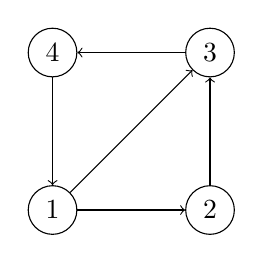
\begin{tikzpicture}
        \node[draw, circle] (v1) at (0, 0) {1};
        \node[draw, circle] (v2) at (2, 0) {2};
        \node[draw, circle] (v3) at (2, 2) {3};
        \node[draw, circle] (v4) at (0, 2) {4};
        \draw[->] (v1) -- (v2);
        \draw[->] (v2) -- (v3);
        \draw[->] (v3) -- (v4);
        \draw[->] (v4) -- (v1);
        \draw[->] (v1) -- (v3);
      \end{tikzpicture}
    \end{column}
    \begin{column}{0.55\textwidth}
      Adjacency matrix:
      \[
        A = \begin{pmatrix}
          0 & 1 & 1 & 0 \\
          0 & 0 & 1 & 0 \\
          0 & 0 & 0 & 1 \\
          1 & 0 & 0 & 0
        \end{pmatrix}
      \]
    \end{column}
  \end{columns}

  \vspace{0.3cm}
  \small
  Weighted graphs: $w : E \to \mathbb{R}$ assigns a weight to each edge.
\end{frame}

% ===========================================================================
\section{Set theory}
% ===========================================================================

\begin{frame}{Sets}
  A set is an unordered collection of unique elements: $\{1, 2, 3\}$.

  \vspace{0.3cm}
  Special sets:
  \begin{itemize}
    \item \textbf{Universe set} $\Omega$: all elements in a given context
    \item \textbf{Empty set} $\emptyset$: no elements
  \end{itemize}
\end{frame}

% ---------------------------------------------------------------------------
\subsection{Set operations}
% ---------------------------------------------------------------------------

\begin{frame}{Set operations}
  \begin{itemize}
    \item \textbf{Union}: $A \cup B$ --- elements in $A$ or $B$
    \item \textbf{Intersection}: $A \cap B$ --- elements in both $A$ and $B$
    \item \textbf{Difference}: $A \setminus B$ --- elements in $A$ but not $B$
    \item \textbf{Complement}: $A^c = \Omega \setminus A$
    \item \textbf{Inclusion}: $A \subseteq B$ --- all elements of $A$ are in $B$
  \end{itemize}
\end{frame}

\begin{frame}{Set operations properties}
  Given sets $A$, $B$, $C$:
  \begin{itemize}
    \item \textit{Commutativity:} $A \cup B = B \cup A$,\quad $A \cap B = B \cap A$
    \item \textit{Associativity:}
      $(A \cup B) \cup C = A \cup (B \cup C)$
    \item \textit{Distributivity:}
      $A \cup (B \cap C) = (A \cup B) \cap (A \cup C)$
  \end{itemize}

  \vspace{0.3cm}
  \textbf{De Morgan's laws:}
  \[
    (A \cup B)^c = A^c \cap B^c
    \qquad
    (A \cap B)^c = A^c \cup B^c
  \]

  \vspace{0.2cm}
  Difference in terms of complement:
  $A \setminus B = A \cap B^c$
\end{frame}

\begin{frame}{Inclusion properties}
  \begin{itemize}
    \item \textit{Reflexivity:} $A \subseteq A$
    \item \textit{Antisymmetry:} $A \subseteq B$ and $B \subseteq A$ iff $A = B$
    \item \textit{Transitivity:} $A \subseteq B$ and $B \subseteq C$ implies
      $A \subseteq C$
  \end{itemize}
\end{frame}

% ---------------------------------------------------------------------------
\subsection{Boolean algebra}
% ---------------------------------------------------------------------------

\begin{frame}{Relation to Boolean algebra}
  \centering
  \rowcolors{2}{black!10!white}{}
  \begin{tabular}{lcc}
    \toprule
    \textbf{Operation} & \textbf{Set} & \textbf{Boolean} \\
    \midrule
    Union / OR & $A \cup B$ & $A \lor B$ \\
    Intersection / AND & $A \cap B$ & $A \land B$ \\
    Complement / NOT & $A^c$ & $\lnot A$ \\
    \bottomrule
  \end{tabular}

  \vspace{0.5cm}
  \raggedright
  De Morgan's laws also hold:
  $\lnot(A \lor B) = \lnot A \land \lnot B$

  \vspace{0.2cm}
  Boolean algebra is the foundation of digital electronics and
  programming control flow.
\end{frame}

% ===========================================================================
\section{Linear algebra}
% ===========================================================================

\begin{frame}{Basic objects}
  \begin{itemize}
    \item \textbf{Vector}: ordered collection of numbers;
      $\vec{v} = [v_i]_{i=1,\ldots,n}$
    \item \textbf{Matrix}: rectangular array;
      $A = (a_{ij})_{i=1,\ldots,n;\; j=1,\ldots,m}$
    \item \textbf{Tensor}: generalization to $k$ indices (rank $k$)
      \begin{itemize}
        \item Scalar: rank 0; Vector: rank 1; Matrix: rank 2
      \end{itemize}
  \end{itemize}
\end{frame}

% ---------------------------------------------------------------------------
\subsection{Operations}
% ---------------------------------------------------------------------------

\begin{frame}{Addition and scalar multiplication}
  \textbf{Addition:}
  \begin{itemize}
    \item Vectors: $(\vec{v} + \vec{w})_i = v_i + w_i$
    \item Matrices: $(A + B)_{ij} = a_{ij} + b_{ij}$
  \end{itemize}

  \vspace{0.3cm}
  \textbf{Scalar multiplication:}
  \begin{itemize}
    \item $(\alpha\vec{v})_i = \alpha v_i$
    \item $(\alpha A)_{ij} = \alpha a_{ij}$
  \end{itemize}
\end{frame}

\begin{frame}{Dot product and matrix multiplication}
  \textbf{Dot product} (inner product):
  \[
    \vec{v} \cdot \vec{w} = \sum_{i=1}^n v_i w_i
  \]

  \vspace{0.3cm}
  \textbf{Matrix multiplication}: $C = AB$, where
  \[
    c_{ij} = \sum_{k=1}^n a_{ik}\, b_{kj}
  \]
  Columns of $A$ must equal rows of $B$.\\
  Vectors are column matrices unless stated otherwise.
\end{frame}

\begin{frame}{Transpose, determinant, inverse}
  \textbf{Transpose}: $(A^T)_{ij} = a_{ji}$

  \vspace{0.3cm}
  \textbf{Determinant}: $\det(A)$ --- measure of signed volume.
  \[
    \begin{vmatrix} a & b \\ c & d \end{vmatrix} = ad - bc
  \]
  $\det(A) \neq 0$ iff $A$ is invertible. $\det(AB) = \det(A)\det(B)$.

  \vspace{0.3cm}
  \textbf{Inverse}: $A A^{-1} = A^{-1} A = I_n$
  \[
    \begin{pmatrix} a & b \\ c & d \end{pmatrix}^{-1}
    = \frac{1}{ad - bc}
    \begin{pmatrix} d & -b \\ -c & a \end{pmatrix}
  \]
\end{frame}

\begin{frame}{Inverse --- general formula}
  \[
    A^{-1} = \frac{1}{\det(A)} \operatorname{adj}(A)
  \]
  where $\operatorname{adj}(A)$ is the transpose of the cofactor matrix.

  \vspace{0.3cm}
  Cofactor of entry $a_{ij}$: determinant of $A$ with row $i$ and
  column $j$ removed, times $(-1)^{i+j}$.
\end{frame}

% ---------------------------------------------------------------------------
\subsection{Systems and eigenvalues}
% ---------------------------------------------------------------------------

\begin{frame}{Systems of linear equations}
  \[
    A\vec{x} = \vec{b}
  \]
  \begin{itemize}
    \item $A$: matrix of constants
    \item $\vec{x}$: vector of unknowns
    \item $\vec{b}$: vector of constants
  \end{itemize}

  \vspace{0.3cm}
  Unique solution iff $A$ is invertible: $\vec{x} = A^{-1}\vec{b}$.
\end{frame}

\begin{frame}{Eigenvalues and eigenvectors}
  An eigenvalue $\lambda$ of $A$ satisfies:
  \[
    A\vec{v} = \lambda\vec{v}
  \]
  for some non-zero eigenvector $\vec{v}$.

  \vspace{0.3cm}
  Eigenvalues are roots of the \textbf{characteristic polynomial}:
  \[
    \det(A - \lambda I_n) = 0
  \]
\end{frame}

% ===========================================================================
\section{Probability}
% ===========================================================================

% ---------------------------------------------------------------------------
\subsection{Axioms and main concepts}
% ---------------------------------------------------------------------------

\begin{frame}{Kolmogorov axioms}
  \begin{enumerate}
    \item $\Prob(A) \geq 0$ for any event $A$
    \item $\Prob(\Omega) = 1$ where $\Omega$ is the sample space
    \item If $A \cap B = \emptyset$:
      $\Prob(A \cup B) = \Prob(A) + \Prob(B)$
  \end{enumerate}

  \vspace{0.3cm}
  \textbf{Sum rule} (non-disjoint):
  \[
    \Prob(A \cup B) = \Prob(A) + \Prob(B) - \Prob(A \cap B)
  \]
\end{frame}

\begin{frame}{Joint, conditional, independence}
  \textbf{Joint probability}:
  $\Prob(A, B) = \Prob(A \cap B)$

  \vspace{0.3cm}
  \textbf{Law of total probability}: if $B_1, \ldots, B_n$ partition
  $\Omega$:
  \[
    \Prob(A) = \sum_{i=1}^n \Prob(A, B_i)
  \]

  \vspace{0.3cm}
  \textbf{Conditional probability}: $\Prob(A \mid B)$

  \vspace{0.3cm}
  \textbf{Independence}: $\Prob(A \mid B) = \Prob(A)$, equivalently
  $\Prob(A, B) = \Prob(A) \cdot \Prob(B)$
\end{frame}

\begin{frame}{Bayes' rule}
  \[
    \Prob(A \mid B) = \frac{\Prob(B \mid A) \cdot \Prob(A)}{\Prob(B)}
  \]

  \vspace{0.3cm}
  One of the most important formulas in probability theory.\\
  Foundation of Bayesian statistics and machine learning.
\end{frame}

% ---------------------------------------------------------------------------
\subsection{Random variables}
% ---------------------------------------------------------------------------

\begin{frame}{Random variables}
  A random variable $X : \Omega \to E$ maps outcomes to values.
  \[
    \Prob(X \in A) = \Prob(\{\omega \in \Omega : X(\omega) \in A\})
  \]

  \vspace{0.3cm}
  \begin{itemize}
    \item $E = \mathbb{R}$: continuous random variable
    \item $E = \mathbb{Z}$: discrete random variable
    \item $X \sim P$: $X$ follows distribution $P$
  \end{itemize}
\end{frame}

\begin{frame}{PMF, PDF, CDF}
  \textbf{Probability mass function} (discrete):
  \[
    p_X(x) = \Prob(X = x)
  \]

  \vspace{0.2cm}
  \textbf{Probability density function} (continuous):
  \[
    \Prob(a \leq X \leq b) = \int_a^b f_X(x)\, dx
  \]

  \vspace{0.2cm}
  \textbf{Cumulative distribution function}:
  \[
    F_X(x) = \Prob(X \leq x)
  \]
\end{frame}

% ---------------------------------------------------------------------------
\subsection{Expectation and moments}
% ---------------------------------------------------------------------------

\begin{frame}{Expectation}
  \[
    \E[X] = \sum_x x \cdot p_X(x)
    \qquad \text{or} \qquad
    \E[X] = \int_{-\infty}^{\infty} x \cdot f_X(x)\, dx
  \]

  \vspace{0.3cm}
  \textbf{Properties} (linearity):
  \begin{align*}
    \E[cX] &= c\,\E[X] \\
    \E[X + c] &= \E[X] + c \\
    \E[X + Y] &= \E[X] + \E[Y]
  \end{align*}

  \vspace{0.2cm}
  General: $\E[g(X)] = \sum_x g(x) \cdot p_X(x)$
  or $\int g(x) \cdot f_X(x)\, dx$.
\end{frame}

\begin{frame}{Variance}
  \[
    \Var(X) = \E\!\left[(X - \E[X])^2\right]
  \]

  \vspace{0.3cm}
  Equivalent form:
  \[
    \Var(X) = \E[X^2] - \E[X]^2
  \]

  \vspace{0.2cm}
  Proof:
  \begin{align*}
    \Var(X) &= \E\!\left[X^2 - 2X\E[X] + \E[X]^2\right] \\
            &= \E[X^2] - 2\E[X]\E[X] + \E[X]^2 \\
            &= \E[X^2] - \E[X]^2
  \end{align*}
\end{frame}

\begin{frame}{Sample statistics}
  \textbf{Sample mean}: $\displaystyle\bar{X} = \frac{1}{n}\sum_{i=1}^n X_i$

  \vspace{0.3cm}
  \textbf{Law of large numbers}:
  $\displaystyle\lim_{n \to \infty} \frac{1}{n}\sum_{i=1}^n X_i = \E[X]$
  \quad (for i.i.d.\ $X_i \sim X$)

  \vspace{0.3cm}
  \textbf{Sample variance}:
  $\displaystyle S^2 = \frac{1}{n-1}\sum_{i=1}^n (X_i - \bar{X})^2$

  \vspace{0.2cm}
  \small Denominator $n-1$ corrects for bias (Bessel's correction).
\end{frame}

\begin{frame}{Higher moments}
  \textbf{$k$-th moment}: $\E[X^k]$

  \vspace{0.3cm}
  \textbf{Sample skewness} (3rd moment):
  \[
    \text{Skewness} = \frac{\frac{1}{n}\sum_{i=1}^n (X_i - \bar{X})^3}{S^3}
  \]
  Zero for symmetric; positive = right-skewed; negative = left-skewed.

  \vspace{0.3cm}
  \textbf{Sample kurtosis} (4th moment):
  \[
    \text{Kurtosis} = \frac{\frac{1}{n}\sum_{i=1}^n (X_i - \bar{X})^4}{S^4} - 3
  \]
  Positive = heavier tails than normal; negative = lighter tails.
\end{frame}

% ---------------------------------------------------------------------------
\subsection{Common distributions}
% ---------------------------------------------------------------------------

\begin{frame}{Bernoulli distribution}
  $X \sim \text{Bern}(p)$, two outcomes (success/failure).

  \vspace{0.3cm}
  \begin{itemize}
    \item $\E[X] = p$
    \item $\Var(X) = p(1 - p)$
  \end{itemize}
\end{frame}

\begin{frame}{Poisson distribution}
  $X \sim \text{Poisson}(\lambda)$, number of events in a fixed interval.

  \vspace{0.3cm}
  PMF:
  \[
    p_X(x) = \frac{e^{-\lambda}\, \lambda^x}{x!}
  \]

  \vspace{0.3cm}
  \begin{itemize}
    \item $\E[X] = \lambda$
    \item $\Var(X) = \lambda$
  \end{itemize}
\end{frame}

\begin{frame}{Normal distribution}
  $X \sim \mathcal{N}(\mu, \sigma^2)$, bell-shaped density.

  \vspace{0.3cm}
  PDF:
  \[
    f_X(x) = \frac{1}{\sqrt{2\pi\sigma^2}}
      \exp\!\left(-\frac{(x - \mu)^2}{2\sigma^2}\right)
  \]

  \vspace{0.3cm}
  \begin{itemize}
    \item $\E[X] = \mu$,\quad $\Var(X) = \sigma^2$
    \item Standard normal: $\mathcal{N}(0, 1)$
  \end{itemize}
\end{frame}

\begin{frame}{Central limit theorem}
  Given $X_1, \ldots, X_n$ i.i.d.\ with mean $\mu$ and finite variance
  $\sigma^2$:
  \[
    \sqrt{n}\,(\bar{X} - \mu) \;\sim\; \mathcal{N}(0, \sigma^2)
    \quad \text{as } n \to \infty
  \]

  \vspace{0.3cm}
  The sample mean is approximately normal for large $n$,
  with mean $\mu$ and variance $\sigma^2 / n$.

  \vspace{0.3cm}
  One of the most important results in probability and statistics.
\end{frame}

\begin{frame}{T distribution}
  $X \sim \mathcal{T}(\nu)$, bell-shaped, heavier tails than normal.

  \vspace{0.3cm}
  \begin{itemize}
    \item $\nu > 0$: degrees of freedom
    \item Location-scale generalization:
      $\mu + \sigma X \sim \mathcal{T}(\mu, \sigma^2, \nu)$
    \item Converges to normal:
      $\displaystyle\lim_{\nu \to \infty} \mathcal{T}(\nu) = \mathcal{N}(0, 1)$
  \end{itemize}
\end{frame}

\begin{frame}{Gamma distribution}
  $X \sim \text{Gamma}(\alpha, \beta)$, right-skewed density.

  \vspace{0.3cm}
  PDF:
  \[
    f_X(x) = \frac{\beta^\alpha\, x^{\alpha - 1}\, e^{-\beta x}}
      {\Gamma(\alpha)}
  \]
  where $\displaystyle\Gamma(\alpha) = \int_0^\infty t^{\alpha-1}\, e^{-t}\, dt$.

  \vspace{0.3cm}
  Commonly used as a \textbf{conjugate prior} in Bayesian analysis.
\end{frame}

% ---------------------------------------------------------------------------
\subsection{Combinatorics}
% ---------------------------------------------------------------------------

\begin{frame}{Permutations and combinations}
  \textbf{Factorial}:
  $n! = n \cdot (n-1) \cdots 2 \cdot 1$,\quad $0! = 1$

  \vspace{0.3cm}
  \textbf{Permutation}: number of arrangements of $n$ elements $= n!$

  \vspace{0.3cm}
  \textbf{Combination}: number of ways to choose $k$ from $n$:
  \[
    \binom{n}{k} = \frac{n!}{k!\,(n - k)!}
  \]
\end{frame}

% ---- End ----

\begin{frame}[standout]
  Questions?
\end{frame}

\end{document}

\chapter{Topics on learning machines}
\label[appendix]{chap:learning-machines}
\glsresetall


\chapterprecishere{Oh, the depth of the riches and wisdom and knowledge of God! How
  unsearchable are his judgments and how inscrutable his ways!
  \par\raggedleft--- \textup{Romans 11:33} (ESV)}

This appendix is under construction.  Topics like the kernel trick, back-propagation, and
other machine learning algorithms will be discussed here.

{}
\clearpage

\section{Multi-layer perceptron}
\label{sec:mlp}

The \gls{mlp} is a non-linear \gls{classifier} that generates a set of hyperplanes
that separates the classes.  In order to simplify understanding, consider
that the activation function of the hidden layer is the discrete step function
\begin{equation*}
  \sigma(x) = \begin{cases}
    1 & \text{if } x > 0 \\
    0 & \text{otherwise.}
  \end{cases}
\end{equation*}
A model with two neurons in the hidden layer (effectively the combination of three
perceptrons) is
\begin{multline*}
  f(x_1, x_2; \theta = \left\{ \vec{w}^{(1)}, \vec{w}^{(2)}, \vec{w}^{(3)} \right\}) = \\
  \sigma\left(
    \vec{w}^{(3)} \cdot \left[1, \sigma(\vec{w}^{(1)} \cdot \vec{x}), \sigma(\vec{w}^{(2)} \cdot \vec{x})\right]
  \right)\text{.}
\end{multline*}

The parameters $\vec{w}^{(1)}$ and $\vec{w}^{(2)}$ represent the hyperplanes that separate
the classes in the hidden layer, and $\vec{w}^{(3)}$ represents how the hyperplanes are
combined to generate the output.  If we set weights $\vec{w}^{(1)} = [-0.5, 1, -1]$ (like the
perceptron in the previous example) and $\vec{w}^{(2)} = [-0.5, -1, 1]$, we use the third neuron
to combine the results of the first two neurons.  This way, a possible solution for the
XOR problem is setting $\vec{w}^{(3)} = [0, 1, 1]$.

\begin{figurebox}[label=fig:mlp]{MLP class boundaries for the XOR problem.}
  \centering
  \begin{tikzpicture}
    \begin{axis}[
        axis x line=bottom,
        axis y line=left,
        xlabel={$x_1$},
        ylabel={$x_2$},
        width=0.6\textwidth,
        height=0.6\textwidth,
        xtick={0, 1},
        ytick={0, 1},
        xmin=-0.5, xmax=1.5,
        ymin=-0.5, ymax=1.5,
      ]
      \addplot+[only marks, mark=+, color=black, mark size=3pt] coordinates {
        (0, 1) (1, 0)
      };
      \addplot+[only marks, mark=-, color=black, mark size=3pt] coordinates {
        (0, 0) (1, 1)
      };
      \addplot+[domain=0:1.5, mark=none, black, thick] {-0.5 + x};
      \addplot+[domain=-0.5:1.5, mark=none, black, thick] {0.5 + x};
    \end{axis}
  \end{tikzpicture}
  \tcblower
  \Gls{mlp} with two neurons in the hidden layer generates two linear hyperplanes that
  separate the classes, effectively solving the XOR problem.
\end{figurebox}

\begin{tablebox}[label=tab:xor-mlp]{Truth table for the predictions of the MLP.}
  \centering
  \rowcolors{2}{black!10!white}{}
  \begin{tabular}{ccc|cccc}
    \toprule
    $x_1$ & $x_2$ & $y$ & \nth{1} neuron & \nth{2} neuron & $\hat{y}$ \\
    \midrule
    0 & 0 & 0 & 0 & 0 & 0 \\
    0 & 1 & 1 & 0 & 1 & 1 \\
    1 & 0 & 1 & 1 & 0 & 1 \\
    1 & 1 & 0 & 0 & 0 & 0 \\
    \bottomrule
  \end{tabular}
  \tcblower
  Predictions of the \gls{mlp} for the XOR problem.  The output of the \nth{1} and \nth{2}
  neurons are hyperplanes that separate the classes in the hidden layer, which are
  combined by the \nth{3} neuron to generate the correct output.
\end{tablebox}

\Cref{fig:mlp,tab:xor-mlp} show the class boundaries and the predictions of the MLP for
the XOR problem.

Note that there are many possible solutions for the XOR problem using the MLP.
Learning strategies like back-propagation are used to find the optimal parameters for
the model and \gls{regularization} techniques, like $l_1$ and $l_2$ \gls{regularization}, are used to
prevent overfitting.

% TODO: backpropagation and regularization
% TODO: talk about deep learning

Deep learning is the study of neural networks with many layers.  The idea is to use many
layers to learn not only the boundaries that separate the classes (or the function that
maps inputs and outputs) but also the features that are relevant to the problem.
A complete discussion of deep learning can be found in
\textcite{Goodfellow2016}\footfullcite{Goodfellow2016}.

\clearpage
\section{Decision trees}

The decision tree is a non-linear \gls{classifier} that generates a set of hyperplanes that
are orthogonal to the axes.  Consider the decision tree in \cref{fig:tree-and}.

\begin{figurebox}[label=fig:tree-and]{Decision tree representation.}
  \centering
  \begin{tikzpicture}
    \node[decision] (x1) at (0, 0) {$x_1$};
    \node[block] (n1) at (-2, -1.5) {$\hat{y} = 0$};
    \node[decision] (x2) at (2, -1.5) {$x_2$};
    \node[block] (n2) at (0, -3) {$\hat{y} = 0$};
    \node[block] (p) at (4, -3) {$\hat{y} = 1$};

    \draw (x1) -| (n1) node [midway, above] {$\leq 0.5$};
    \draw (x1) -| (x2) node [midway, above] {$>0.5$};
    \draw (x2) -| (n2) node [midway, above] {$\leq 0.5$};
    \draw (x2) -| (p) node [midway, above] {$>0.5$};
  \end{tikzpicture}
  \tcblower
  The decision tree that solves the AND problem.
\end{figurebox}

\begin{figurebox}[label=fig:tree-bias]{Decision tree spatial representation.}
  \centering
  \begin{tikzpicture}
    \begin{axis}[
        axis x line=bottom,
        axis y line=left,
        xlabel={$x_1$},
        ylabel={$x_2$},
        width=0.6\textwidth,
        height=0.6\textwidth,
        xtick={0, 1},
        ytick={0, 1},
        xmin=-0.5, xmax=1.5,
        ymin=-0.5, ymax=1.5,
      ]
      \addplot+[only marks, mark=+, black, mark size=3pt] coordinates {
        (1, 1)
      };
      \addplot+[only marks, mark=-, black, mark size=3pt] coordinates {
        (0, 0) (0, 1) (1, 0)
      };
      \addplot+[domain=0.5:1.5, mark=none, black, thick] {0.5};
      \addplot+[mark=none, black, thick] coordinates {(0.5, -0.5) (0.5, 1.5)};
    \end{axis}
  \end{tikzpicture}
  \tcblower
  Decision trees assume that the classes can be separated with
  hyperplanes orthogonal to the axes.
\end{figurebox}

The spatial representation of the decision tree is shown in \cref{fig:tree-bias}.
Decision trees are a type of \gls{classifier} that generates a set of hyperplanes orthogonal to the axes.

Decision trees are nonparametric models, one can easily increase the depth of the tree to
fit the data, generating as many hyperplanes as necessary to separate the classes.
Training a decision tree with a large depth can lead to overfitting, so it is important to
use techniques like depth limit and pruning to prevent this from happening.

% \subsection{$k$-nearest neighbors learning bias}
%
% The $k$-nearest neighbors ($k$-NN) is a non-linear nonparametric classifier that
% generate arbitrarily complex decision boundaries by ``memoring'' the training data.
% The behavior of the boundaries depends on the value of $k$ and the distance metric one
% uses to find the nearest neighbors of a point.
%
% \begin{figurebox}[label=fig:1nn-bias]{1-NN learning bias.}
%   \centering
%   \begin{tikzpicture}
%     \begin{axis}[
%         axis x line=bottom,
%         axis y line=left,
%         xlabel={$x_1$},
%         ylabel={$x_2$},
%         width=0.6\textwidth,
%         height=0.6\textwidth,
%         xtick={0, 1},
%         ytick={0, 1},
%         grid=both,
%         xmin=-0.5, xmax=1.5,
%         ymin=-0.5, ymax=1.5,
%       ]
%       \addplot+[only marks, mark=+, mark size=3pt] coordinates {
%         (1, 1)
%       };
%       \addplot+[only marks, mark=*, mark size=3pt] coordinates {
%         (0, 0) (0, 1) (1, 0)
%       };
%       \addplot+[domain=0.5:1.5, mark=none, black, thick] {0.5};
%       \addplot+[mark=none, black, thick] coordinates {(0.5, 0.5) (0.5, 1.5)};
%     \end{axis}
%   \end{tikzpicture}
%   \tcblower
%   In this particular case, the 1-NN boundaries match the decision tree boundaries.
% \end{figurebox}
%
% As $k$ increases the boundaries become smoother:
% \href{https://images.squarespace-cdn.com/content/v1/5d782753c70af105c29a9b14/1580261947016-XODPUVKWPGGMJJMAXSNF/Screen+Shot+2020-01-28+at+8.38.55+PM.png}{example}.
%
% See illustration: \href{https://scikit-learn.org/stable/auto_examples/classification/plot_classifier_comparison.html}{here}.

% vim: spell spelllang=en


\backmatter

\printglossary

\printbibliography[heading=bibintoc]

\end{document}
